\documentclass[twoside]{book}

% Packages required by doxygen
\usepackage{calc}
\usepackage{doxygen}
\usepackage{graphicx}
\usepackage[utf8]{inputenc}
\usepackage{makeidx}
\usepackage{multicol}
\usepackage{multirow}
\usepackage{textcomp}
\usepackage[table]{xcolor}

% Font selection
\usepackage[T1]{fontenc}
\usepackage{mathptmx}
\usepackage[scaled=.90]{helvet}
\usepackage{courier}
\usepackage{amssymb}
\usepackage{sectsty}
\renewcommand{\familydefault}{\sfdefault}
\allsectionsfont{%
  \fontseries{bc}\selectfont%
  \color{darkgray}%
}
\renewcommand{\DoxyLabelFont}{%
  \fontseries{bc}\selectfont%
  \color{darkgray}%
}

% Page & text layout
\usepackage{geometry}
\geometry{%
  a4paper,%
  top=2.5cm,%
  bottom=2.5cm,%
  left=2.5cm,%
  right=2.5cm%
}
\tolerance=750
\hfuzz=15pt
\hbadness=750
\setlength{\emergencystretch}{15pt}
\setlength{\parindent}{0cm}
\setlength{\parskip}{0.2cm}
\makeatletter
\renewcommand{\paragraph}{%
  \@startsection{paragraph}{4}{0ex}{-1.0ex}{1.0ex}{%
    \normalfont\normalsize\bfseries\SS@parafont%
  }%
}
\renewcommand{\subparagraph}{%
  \@startsection{subparagraph}{5}{0ex}{-1.0ex}{1.0ex}{%
    \normalfont\normalsize\bfseries\SS@subparafont%
  }%
}
\makeatother

% Headers & footers
\usepackage{fancyhdr}
\pagestyle{fancyplain}
\fancyhead[LE]{\fancyplain{}{\bfseries\thepage}}
\fancyhead[CE]{\fancyplain{}{}}
\fancyhead[RE]{\fancyplain{}{\bfseries\leftmark}}
\fancyhead[LO]{\fancyplain{}{\bfseries\rightmark}}
\fancyhead[CO]{\fancyplain{}{}}
\fancyhead[RO]{\fancyplain{}{\bfseries\thepage}}
\fancyfoot[LE]{\fancyplain{}{}}
\fancyfoot[CE]{\fancyplain{}{}}
\fancyfoot[RE]{\fancyplain{}{\bfseries\scriptsize Generated on Fri Dec 6 2013 21\-:21\-:26 for My Project by Doxygen }}
\fancyfoot[LO]{\fancyplain{}{\bfseries\scriptsize Generated on Fri Dec 6 2013 21\-:21\-:26 for My Project by Doxygen }}
\fancyfoot[CO]{\fancyplain{}{}}
\fancyfoot[RO]{\fancyplain{}{}}
\renewcommand{\footrulewidth}{0.4pt}
\renewcommand{\chaptermark}[1]{%
  \markboth{#1}{}%
}
\renewcommand{\sectionmark}[1]{%
  \markright{\thesection\ #1}%
}

% Indices & bibliography
\usepackage{natbib}
\usepackage[titles]{tocloft}
\setcounter{tocdepth}{3}
\setcounter{secnumdepth}{5}
\makeindex

% Hyperlinks (required, but should be loaded last)
\usepackage{ifpdf}
\ifpdf
  \usepackage[pdftex,pagebackref=true]{hyperref}
\else
  \usepackage[ps2pdf,pagebackref=true]{hyperref}
\fi
\hypersetup{%
  colorlinks=true,%
  linkcolor=blue,%
  citecolor=blue,%
  unicode%
}

% Custom commands
\newcommand{\clearemptydoublepage}{%
  \newpage{\pagestyle{empty}\cleardoublepage}%
}


%===== C O N T E N T S =====

\begin{document}

% Titlepage & ToC
\hypersetup{pageanchor=false}
\pagenumbering{roman}
\begin{titlepage}
\vspace*{7cm}
\begin{center}%
{\Large My Project }\\
\vspace*{1cm}
{\large Generated by Doxygen 1.8.5}\\
\vspace*{0.5cm}
{\small Fri Dec 6 2013 21:21:26}\\
\end{center}
\end{titlepage}
\clearemptydoublepage
\tableofcontents
\clearemptydoublepage
\pagenumbering{arabic}
\hypersetup{pageanchor=true}

%--- Begin generated contents ---
\chapter{Hierarchical Index}
\section{Class Hierarchy}
This inheritance list is sorted roughly, but not completely, alphabetically\-:\begin{DoxyCompactList}
\item \contentsline{section}{anim\-Items}{\pageref{classanim_items}}{}
\item \contentsline{section}{attack\-List}{\pageref{classattack_list}}{}
\item \contentsline{section}{attackmove}{\pageref{classattackmove}}{}
\begin{DoxyCompactList}
\item \contentsline{section}{brokengun}{\pageref{classbrokengun}}{}
\item \contentsline{section}{brokenshot}{\pageref{classbrokenshot}}{}
\item \contentsline{section}{Hookslash}{\pageref{class_hookslash}}{}
\item \contentsline{section}{shotgun}{\pageref{classshotgun}}{}
\item \contentsline{section}{swordslash}{\pageref{classswordslash}}{}
\item \contentsline{section}{xgun}{\pageref{classxgun}}{}
\end{DoxyCompactList}
\item \contentsline{section}{Character}{\pageref{class_character}}{}
\item Q\-Dialog\begin{DoxyCompactList}
\item \contentsline{section}{attackframe}{\pageref{classattackframe}}{}
\item \contentsline{section}{Pause}{\pageref{class_pause}}{}
\item \contentsline{section}{worldmap}{\pageref{classworldmap}}{}
\end{DoxyCompactList}
\item Q\-Graphics\-Item\begin{DoxyCompactList}
\item \contentsline{section}{Back\-From\-End}{\pageref{class_back_from_end}}{}
\item \contentsline{section}{Back\-From\-In\-Store}{\pageref{class_back_from_in_store}}{}
\item \contentsline{section}{Back\-From\-Store}{\pageref{class_back_from_store}}{}
\item \contentsline{section}{In\-Store}{\pageref{class_in_store}}{}
\item \contentsline{section}{Map\-Enemy}{\pageref{class_map_enemy}}{}
\item \contentsline{section}{Map\-Hero}{\pageref{class_map_hero}}{}
\item \contentsline{section}{Mega\-Enemy}{\pageref{class_mega_enemy}}{}
\item \contentsline{section}{Mini\-Enemy}{\pageref{class_mini_enemy}}{}
\item \contentsline{section}{To\-End}{\pageref{class_to_end}}{}
\item \contentsline{section}{To\-Store}{\pageref{class_to_store}}{}
\end{DoxyCompactList}
\item Q\-Graphics\-View\begin{DoxyCompactList}
\item \contentsline{section}{Graphics\-View}{\pageref{class_graphics_view}}{}
\end{DoxyCompactList}
\item Q\-Main\-Window\begin{DoxyCompactList}
\item \contentsline{section}{Main\-Window}{\pageref{class_main_window}}{}
\end{DoxyCompactList}
\item Q\-Object\begin{DoxyCompactList}
\item \contentsline{section}{Enemy}{\pageref{class_enemy}}{}
\begin{DoxyCompactList}
\item \contentsline{section}{Bomber}{\pageref{class_bomber}}{}
\item \contentsline{section}{Cannon}{\pageref{class_cannon}}{}
\item \contentsline{section}{Hunter}{\pageref{class_hunter}}{}
\item \contentsline{section}{Skeleton}{\pageref{class_skeleton}}{}
\item \contentsline{section}{swordsman}{\pageref{classswordsman}}{}
\end{DoxyCompactList}
\end{DoxyCompactList}
\item \contentsline{section}{qt\-\_\-meta\-\_\-stringdata\-\_\-\-Battle\-Pause\-\_\-t}{\pageref{structqt__meta__stringdata___battle_pause__t}}{}
\item \contentsline{section}{qt\-\_\-meta\-\_\-stringdata\-\_\-\-Main\-Window\-\_\-t}{\pageref{structqt__meta__stringdata___main_window__t}}{}
\item \contentsline{section}{qt\-\_\-meta\-\_\-stringdata\-\_\-\-Pause\-\_\-t}{\pageref{structqt__meta__stringdata___pause__t}}{}
\item \contentsline{section}{qt\-\_\-meta\-\_\-stringdata\-\_\-worldmap\-\_\-t}{\pageref{structqt__meta__stringdata__worldmap__t}}{}
\item Q\-Widget\begin{DoxyCompactList}
\item \contentsline{section}{Circle\-Widget}{\pageref{class_circle_widget}}{}
\item \contentsline{section}{Wiggly\-Widget}{\pageref{class_wiggly_widget}}{}
\end{DoxyCompactList}
\item \contentsline{section}{Ui\-\_\-\-Battle\-Pause}{\pageref{class_ui___battle_pause}}{}
\begin{DoxyCompactList}
\item \contentsline{section}{Ui\-:\-:Battle\-Pause}{\pageref{class_ui_1_1_battle_pause}}{}
\end{DoxyCompactList}
\item \contentsline{section}{Ui\-\_\-\-Main\-Window}{\pageref{class_ui___main_window}}{}
\begin{DoxyCompactList}
\item \contentsline{section}{Ui\-:\-:Main\-Window}{\pageref{class_ui_1_1_main_window}}{}
\end{DoxyCompactList}
\item \contentsline{section}{Ui\-\_\-\-Pause}{\pageref{class_ui___pause}}{}
\begin{DoxyCompactList}
\item \contentsline{section}{Ui\-:\-:Pause}{\pageref{class_ui_1_1_pause}}{}
\end{DoxyCompactList}
\item \contentsline{section}{Ui\-\_\-worldmap}{\pageref{class_ui__worldmap}}{}
\begin{DoxyCompactList}
\item \contentsline{section}{Ui\-:\-:worldmap}{\pageref{class_ui_1_1worldmap}}{}
\end{DoxyCompactList}
\end{DoxyCompactList}

\chapter{Class Index}
\section{Class List}
Here are the classes, structs, unions and interfaces with brief descriptions\-:\begin{DoxyCompactList}
\item\contentsline{section}{\hyperlink{classanim_items}{anim\-Items} }{\pageref{classanim_items}}{}
\item\contentsline{section}{\hyperlink{classattackframe}{attackframe} }{\pageref{classattackframe}}{}
\item\contentsline{section}{\hyperlink{classattack_list}{attack\-List} }{\pageref{classattack_list}}{}
\item\contentsline{section}{\hyperlink{classattackmove}{attackmove} }{\pageref{classattackmove}}{}
\item\contentsline{section}{\hyperlink{class_back_from_end}{Back\-From\-End} }{\pageref{class_back_from_end}}{}
\item\contentsline{section}{\hyperlink{class_back_from_in_store}{Back\-From\-In\-Store} }{\pageref{class_back_from_in_store}}{}
\item\contentsline{section}{\hyperlink{class_back_from_store}{Back\-From\-Store} }{\pageref{class_back_from_store}}{}
\item\contentsline{section}{\hyperlink{class_ui_1_1_battle_pause}{Ui\-::\-Battle\-Pause} }{\pageref{class_ui_1_1_battle_pause}}{}
\item\contentsline{section}{\hyperlink{class_bomber}{Bomber} }{\pageref{class_bomber}}{}
\item\contentsline{section}{\hyperlink{classbrokengun}{brokengun} }{\pageref{classbrokengun}}{}
\item\contentsline{section}{\hyperlink{classbrokenshot}{brokenshot} }{\pageref{classbrokenshot}}{}
\item\contentsline{section}{\hyperlink{class_cannon}{Cannon} }{\pageref{class_cannon}}{}
\item\contentsline{section}{\hyperlink{class_character}{Character} }{\pageref{class_character}}{}
\item\contentsline{section}{\hyperlink{class_circle_widget}{Circle\-Widget} \\*\mbox{[}0\mbox{]} }{\pageref{class_circle_widget}}{}
\item\contentsline{section}{\hyperlink{class_enemy}{Enemy} }{\pageref{class_enemy}}{}
\item\contentsline{section}{\hyperlink{class_graphics_view}{Graphics\-View} }{\pageref{class_graphics_view}}{}
\item\contentsline{section}{\hyperlink{class_hookslash}{Hookslash} }{\pageref{class_hookslash}}{}
\item\contentsline{section}{\hyperlink{class_hunter}{Hunter} }{\pageref{class_hunter}}{}
\item\contentsline{section}{\hyperlink{class_in_store}{In\-Store} }{\pageref{class_in_store}}{}
\item\contentsline{section}{\hyperlink{class_main_window}{Main\-Window} }{\pageref{class_main_window}}{}
\item\contentsline{section}{\hyperlink{class_ui_1_1_main_window}{Ui\-::\-Main\-Window} }{\pageref{class_ui_1_1_main_window}}{}
\item\contentsline{section}{\hyperlink{class_map_enemy}{Map\-Enemy} }{\pageref{class_map_enemy}}{}
\item\contentsline{section}{\hyperlink{class_map_hero}{Map\-Hero} }{\pageref{class_map_hero}}{}
\item\contentsline{section}{\hyperlink{class_mega_enemy}{Mega\-Enemy} }{\pageref{class_mega_enemy}}{}
\item\contentsline{section}{\hyperlink{class_mini_enemy}{Mini\-Enemy} }{\pageref{class_mini_enemy}}{}
\item\contentsline{section}{\hyperlink{class_ui_1_1_pause}{Ui\-::\-Pause} }{\pageref{class_ui_1_1_pause}}{}
\item\contentsline{section}{\hyperlink{class_pause}{Pause} \\*This is a \hyperlink{class_pause}{Pause} class. This class will build the pause menu on some key event }{\pageref{class_pause}}{}
\item\contentsline{section}{\hyperlink{structqt__meta__stringdata___battle_pause__t}{qt\-\_\-meta\-\_\-stringdata\-\_\-\-Battle\-Pause\-\_\-t} }{\pageref{structqt__meta__stringdata___battle_pause__t}}{}
\item\contentsline{section}{\hyperlink{structqt__meta__stringdata___main_window__t}{qt\-\_\-meta\-\_\-stringdata\-\_\-\-Main\-Window\-\_\-t} }{\pageref{structqt__meta__stringdata___main_window__t}}{}
\item\contentsline{section}{\hyperlink{structqt__meta__stringdata___pause__t}{qt\-\_\-meta\-\_\-stringdata\-\_\-\-Pause\-\_\-t} }{\pageref{structqt__meta__stringdata___pause__t}}{}
\item\contentsline{section}{\hyperlink{structqt__meta__stringdata__worldmap__t}{qt\-\_\-meta\-\_\-stringdata\-\_\-worldmap\-\_\-t} }{\pageref{structqt__meta__stringdata__worldmap__t}}{}
\item\contentsline{section}{\hyperlink{classshotgun}{shotgun} }{\pageref{classshotgun}}{}
\item\contentsline{section}{\hyperlink{class_skeleton}{Skeleton} }{\pageref{class_skeleton}}{}
\item\contentsline{section}{\hyperlink{classswordslash}{swordslash} }{\pageref{classswordslash}}{}
\item\contentsline{section}{\hyperlink{classswordsman}{swordsman} }{\pageref{classswordsman}}{}
\item\contentsline{section}{\hyperlink{class_to_end}{To\-End} }{\pageref{class_to_end}}{}
\item\contentsline{section}{\hyperlink{class_to_store}{To\-Store} }{\pageref{class_to_store}}{}
\item\contentsline{section}{\hyperlink{class_ui___battle_pause}{Ui\-\_\-\-Battle\-Pause} }{\pageref{class_ui___battle_pause}}{}
\item\contentsline{section}{\hyperlink{class_ui___main_window}{Ui\-\_\-\-Main\-Window} }{\pageref{class_ui___main_window}}{}
\item\contentsline{section}{\hyperlink{class_ui___pause}{Ui\-\_\-\-Pause} }{\pageref{class_ui___pause}}{}
\item\contentsline{section}{\hyperlink{class_ui__worldmap}{Ui\-\_\-worldmap} }{\pageref{class_ui__worldmap}}{}
\item\contentsline{section}{\hyperlink{class_wiggly_widget}{Wiggly\-Widget} \\*\mbox{[}0\mbox{]} }{\pageref{class_wiggly_widget}}{}
\item\contentsline{section}{\hyperlink{classworldmap}{worldmap} }{\pageref{classworldmap}}{}
\item\contentsline{section}{\hyperlink{class_ui_1_1worldmap}{Ui\-::worldmap} }{\pageref{class_ui_1_1worldmap}}{}
\item\contentsline{section}{\hyperlink{classxgun}{xgun} }{\pageref{classxgun}}{}
\end{DoxyCompactList}

\chapter{Class Documentation}
\hypertarget{classanim_items}{\section{anim\-Items Class Reference}
\label{classanim_items}\index{anim\-Items@{anim\-Items}}
}
\subsection*{Public Member Functions}
\begin{DoxyCompactItemize}
\item 
\hypertarget{classanim_items_a41a97b9ae416051cb9203499577c77af}{void \hyperlink{classanim_items_a41a97b9ae416051cb9203499577c77af}{reset} ()}\label{classanim_items_a41a97b9ae416051cb9203499577c77af}

\begin{DoxyCompactList}\small\item\em \hyperlink{classanim_items_a41a97b9ae416051cb9203499577c77af}{anim\-Items\-::reset}, resets the hits to zero \end{DoxyCompactList}\item 
int \hyperlink{classanim_items_a8da8e0816cfb6288fbd122e5f2e1b6ce}{get\-Hit} (int i, int j)
\begin{DoxyCompactList}\small\item\em \hyperlink{classanim_items_a8da8e0816cfb6288fbd122e5f2e1b6ce}{anim\-Items\-::get\-Hit} takes i and j and gets hit from hits\mbox{[}\mbox{]} \end{DoxyCompactList}\item 
void \hyperlink{classanim_items_a1764237122104d10d12b4300fbe091fe}{set\-Hit} (int i, int j, int val)
\begin{DoxyCompactList}\small\item\em \hyperlink{classanim_items_a1764237122104d10d12b4300fbe091fe}{anim\-Items\-::set\-Hit} sets hit to value (should be 1 for hit) \end{DoxyCompactList}\end{DoxyCompactItemize}


\subsection{Member Function Documentation}
\hypertarget{classanim_items_a8da8e0816cfb6288fbd122e5f2e1b6ce}{\index{anim\-Items@{anim\-Items}!get\-Hit@{get\-Hit}}
\index{get\-Hit@{get\-Hit}!animItems@{anim\-Items}}
\subsubsection[{get\-Hit}]{\setlength{\rightskip}{0pt plus 5cm}int anim\-Items\-::get\-Hit (
\begin{DoxyParamCaption}
\item[{int}]{i, }
\item[{int}]{j}
\end{DoxyParamCaption}
)}}\label{classanim_items_a8da8e0816cfb6288fbd122e5f2e1b6ce}


\hyperlink{classanim_items_a8da8e0816cfb6288fbd122e5f2e1b6ce}{anim\-Items\-::get\-Hit} takes i and j and gets hit from hits\mbox{[}\mbox{]} 


\begin{DoxyParams}{Parameters}
{\em i} & \\
\hline
{\em j} & \\
\hline
\end{DoxyParams}
\begin{DoxyReturn}{Returns}

\end{DoxyReturn}
\hypertarget{classanim_items_a1764237122104d10d12b4300fbe091fe}{\index{anim\-Items@{anim\-Items}!set\-Hit@{set\-Hit}}
\index{set\-Hit@{set\-Hit}!animItems@{anim\-Items}}
\subsubsection[{set\-Hit}]{\setlength{\rightskip}{0pt plus 5cm}void anim\-Items\-::set\-Hit (
\begin{DoxyParamCaption}
\item[{int}]{i, }
\item[{int}]{j, }
\item[{int}]{val}
\end{DoxyParamCaption}
)}}\label{classanim_items_a1764237122104d10d12b4300fbe091fe}


\hyperlink{classanim_items_a1764237122104d10d12b4300fbe091fe}{anim\-Items\-::set\-Hit} sets hit to value (should be 1 for hit) 


\begin{DoxyParams}{Parameters}
{\em i} & \\
\hline
{\em j} & \\
\hline
{\em val} & \\
\hline
\end{DoxyParams}


The documentation for this class was generated from the following files\-:\begin{DoxyCompactItemize}
\item 
animitems.\-h\item 
animitems.\-cpp\end{DoxyCompactItemize}

\hypertarget{classattackframe}{\section{attackframe Class Reference}
\label{classattackframe}\index{attackframe@{attackframe}}
}
Inheritance diagram for attackframe\-:\begin{figure}[H]
\begin{center}
\leavevmode
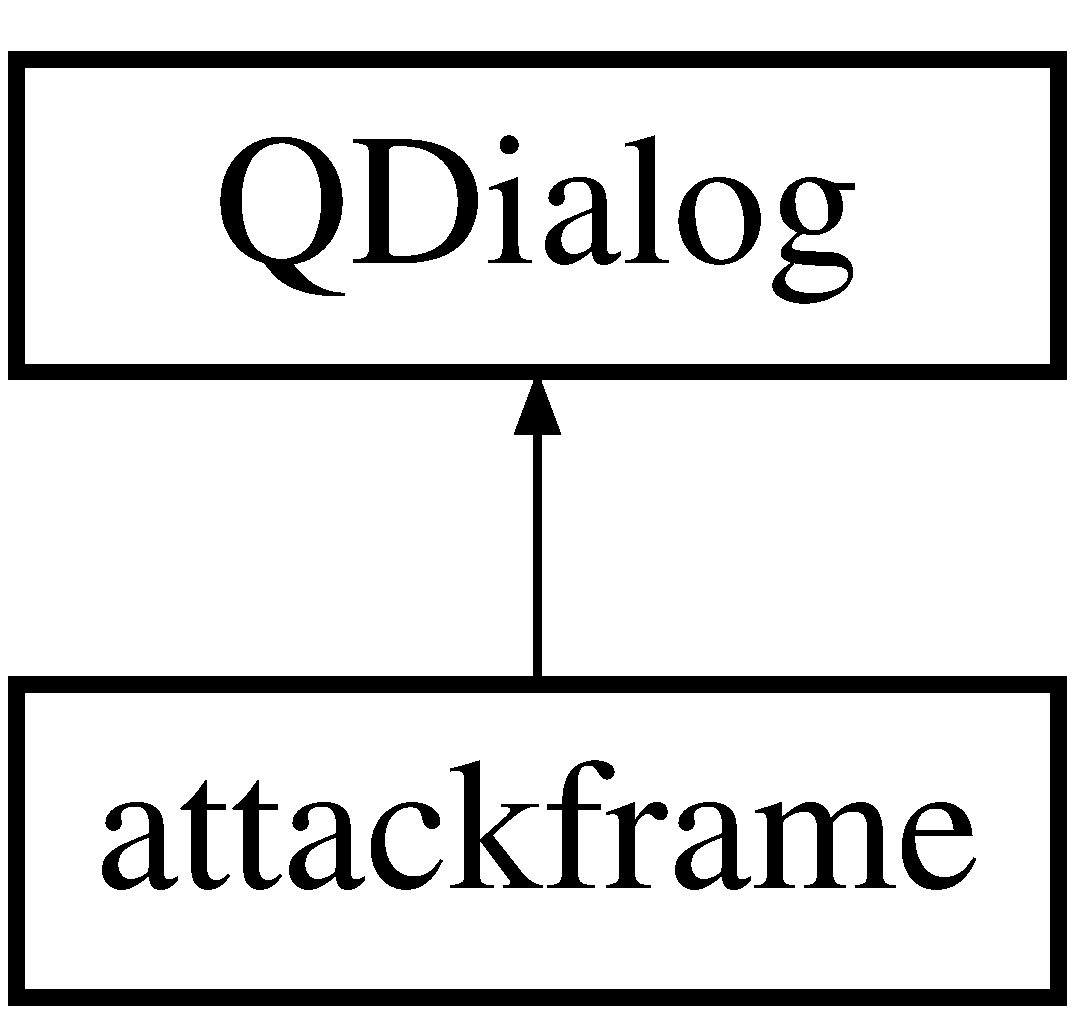
\includegraphics[height=2.000000cm]{classattackframe}
\end{center}
\end{figure}
\subsection*{Public Member Functions}
\begin{DoxyCompactItemize}
\item 
\hyperlink{classattackframe_a4093d85f3f3400f00cca4ffdb87c858d}{attackframe} (Q\-Widget $\ast$parent=0)
\begin{DoxyCompactList}\small\item\em \hyperlink{classattackframe_a4093d85f3f3400f00cca4ffdb87c858d}{attackframe\-::attackframe} sets up the Hero, Main Attack, Attack List, Animation items and event filter \end{DoxyCompactList}\item 
void \hyperlink{classattackframe_a708bc137367ff5315da0a7f62c1f8494}{start\-Battle} (char etype1, int ehp1, int ex1, int ey1, char etype2, int ehp2, int ex2, int ey2, char etype3, int ehp3, int ex3, int ey3)
\begin{DoxyCompactList}\small\item\em start\-Battle sets up game to fight off enemies \end{DoxyCompactList}\item 
\hyperlink{class_character}{Character} $\ast$ \hyperlink{classattackframe_a1806dca8de141292ba69c8d79609f8d6}{get\-Hero} ()
\begin{DoxyCompactList}\small\item\em get\-Hero method is used to access Hero properties \end{DoxyCompactList}\end{DoxyCompactItemize}
\subsection*{Public Attributes}
\begin{DoxyCompactItemize}
\item 
\hypertarget{classattackframe_a419e0dcfdbae9999b46144a90fff2e37}{int {\bfseries num\-Potions}}\label{classattackframe_a419e0dcfdbae9999b46144a90fff2e37}

\item 
\hypertarget{classattackframe_abb1578b5fc8d2357009a51381db2425a}{\hyperlink{class_character}{Character} $\ast$ {\bfseries Hero}}\label{classattackframe_abb1578b5fc8d2357009a51381db2425a}

\end{DoxyCompactItemize}
\subsection*{Protected Member Functions}
\begin{DoxyCompactItemize}
\item 
\hypertarget{classattackframe_a68df3f4ae2ac6b1a1773d3846cb033cb}{bool {\bfseries event\-Filter} (Q\-Object $\ast$obj, Q\-Event $\ast$event)}\label{classattackframe_a68df3f4ae2ac6b1a1773d3846cb033cb}

\end{DoxyCompactItemize}


\subsection{Constructor \& Destructor Documentation}
\hypertarget{classattackframe_a4093d85f3f3400f00cca4ffdb87c858d}{\index{attackframe@{attackframe}!attackframe@{attackframe}}
\index{attackframe@{attackframe}!attackframe@{attackframe}}
\subsubsection[{attackframe}]{\setlength{\rightskip}{0pt plus 5cm}attackframe\-::attackframe (
\begin{DoxyParamCaption}
\item[{Q\-Widget $\ast$}]{parent = {\ttfamily 0}}
\end{DoxyParamCaption}
)\hspace{0.3cm}{\ttfamily [explicit]}}}\label{classattackframe_a4093d85f3f3400f00cca4ffdb87c858d}


\hyperlink{classattackframe_a4093d85f3f3400f00cca4ffdb87c858d}{attackframe\-::attackframe} sets up the Hero, Main Attack, Attack List, Animation items and event filter 


\begin{DoxyParams}{Parameters}
{\em parent} & \\
\hline
\end{DoxyParams}


\subsection{Member Function Documentation}
\hypertarget{classattackframe_a1806dca8de141292ba69c8d79609f8d6}{\index{attackframe@{attackframe}!get\-Hero@{get\-Hero}}
\index{get\-Hero@{get\-Hero}!attackframe@{attackframe}}
\subsubsection[{get\-Hero}]{\setlength{\rightskip}{0pt plus 5cm}{\bf Character} $\ast$ attackframe\-::get\-Hero (
\begin{DoxyParamCaption}
{}
\end{DoxyParamCaption}
)}}\label{classattackframe_a1806dca8de141292ba69c8d79609f8d6}


get\-Hero method is used to access Hero properties 

\hyperlink{classattackframe_a1806dca8de141292ba69c8d79609f8d6}{attackframe\-::get\-Hero}

\begin{DoxyReturn}{Returns}
pointer to hero

the hero pointer 
\end{DoxyReturn}
\hypertarget{classattackframe_a708bc137367ff5315da0a7f62c1f8494}{\index{attackframe@{attackframe}!start\-Battle@{start\-Battle}}
\index{start\-Battle@{start\-Battle}!attackframe@{attackframe}}
\subsubsection[{start\-Battle}]{\setlength{\rightskip}{0pt plus 5cm}void attackframe\-::start\-Battle (
\begin{DoxyParamCaption}
\item[{char}]{etype1, }
\item[{int}]{ehp1, }
\item[{int}]{ex1, }
\item[{int}]{ey1, }
\item[{char}]{etype2, }
\item[{int}]{ehp2, }
\item[{int}]{ex2, }
\item[{int}]{ey2, }
\item[{char}]{etype3, }
\item[{int}]{ehp3, }
\item[{int}]{ex3, }
\item[{int}]{ey3}
\end{DoxyParamCaption}
)}}\label{classattackframe_a708bc137367ff5315da0a7f62c1f8494}


start\-Battle sets up game to fight off enemies 

\hyperlink{classattackframe_a708bc137367ff5315da0a7f62c1f8494}{attackframe\-::start\-Battle} takes information on enemies and puts them in the write position/level


\begin{DoxyParams}{Parameters}
{\em etype1} & \\
\hline
{\em ehp1} & \\
\hline
{\em ex1} & \\
\hline
{\em ey1} & \\
\hline
{\em etype2} & \\
\hline
{\em ehp2} & \\
\hline
{\em ex2} & \\
\hline
{\em ey2} & \\
\hline
{\em etype3} & \\
\hline
{\em ehp3} & \\
\hline
{\em ex3} & \\
\hline
{\em ey3} & \\
\hline
\end{DoxyParams}


The documentation for this class was generated from the following files\-:\begin{DoxyCompactItemize}
\item 
attackframe.\-h\item 
attackframe.\-cpp\end{DoxyCompactItemize}

\hypertarget{classattack_list}{\section{attack\-List Class Reference}
\label{classattack_list}\index{attack\-List@{attack\-List}}
}
\subsection*{Public Member Functions}
\begin{DoxyCompactItemize}
\item 
\hypertarget{classattack_list_a5edfbea9eb0790b0b2f4bb8a3f39f843}{\hyperlink{classattack_list_a5edfbea9eb0790b0b2f4bb8a3f39f843}{attack\-List} ()}\label{classattack_list_a5edfbea9eb0790b0b2f4bb8a3f39f843}

\begin{DoxyCompactList}\small\item\em \hyperlink{classattack_list_a5edfbea9eb0790b0b2f4bb8a3f39f843}{attack\-List\-::attack\-List} all alists null \end{DoxyCompactList}\item 
void \hyperlink{classattack_list_a8bf01a96841205373a2b179c251f6388}{change\-Move} (int pos, \hyperlink{classattackmove}{attackmove} $\ast$am)
\begin{DoxyCompactList}\small\item\em \hyperlink{classattack_list_a8bf01a96841205373a2b179c251f6388}{attack\-List\-::change\-Move} changes move at pos, used to customise attacks \end{DoxyCompactList}\item 
\hyperlink{classattackmove}{attackmove} $\ast$ \hyperlink{classattack_list_acc9d91fc5f10690b2516c123f13f0342}{get\-Attack} ()
\begin{DoxyCompactList}\small\item\em \hyperlink{classattack_list_acc9d91fc5f10690b2516c123f13f0342}{attack\-List\-::get\-Attack} gets bottom attack \end{DoxyCompactList}\item 
\hyperlink{classattackmove}{attackmove} $\ast$ \hyperlink{classattack_list_a40cb4a49c6403918add3cb4a7043788b}{get\-Attack\-At} (int pos)
\begin{DoxyCompactList}\small\item\em \hyperlink{classattack_list_a40cb4a49c6403918add3cb4a7043788b}{attack\-List\-::get\-Attack\-At} gets attack for printing the list \end{DoxyCompactList}\item 
void \hyperlink{classattack_list_af20e3de4d59258a9e582dc121f0c4bf7}{add\-Move} (\hyperlink{classattackmove}{attackmove} $\ast$am)
\begin{DoxyCompactList}\small\item\em \hyperlink{classattack_list_af20e3de4d59258a9e582dc121f0c4bf7}{attack\-List\-::add\-Move} add attack if theres room \end{DoxyCompactList}\item 
int \hyperlink{classattack_list_a4efb6e2ae4c3c66b30dbd3e0cc9e330f}{get\-Curr} ()
\begin{DoxyCompactList}\small\item\em \hyperlink{classattack_list_a4efb6e2ae4c3c66b30dbd3e0cc9e330f}{attack\-List\-::get\-Curr} \end{DoxyCompactList}\item 
\hypertarget{classattack_list_aef5ebb7304e4f34836a8676398765184}{void \hyperlink{classattack_list_aef5ebb7304e4f34836a8676398765184}{reset} ()}\label{classattack_list_aef5ebb7304e4f34836a8676398765184}

\begin{DoxyCompactList}\small\item\em \hyperlink{classattack_list_aef5ebb7304e4f34836a8676398765184}{attack\-List\-::reset} resets for next battle \end{DoxyCompactList}\item 
\hyperlink{classattackmove}{attackmove} $\ast$ \hyperlink{classattack_list_aa18c2e5fa916658ca18e2d6c94c6fd25}{take\-Move\-At} (int pos)
\begin{DoxyCompactList}\small\item\em \hyperlink{classattack_list_aa18c2e5fa916658ca18e2d6c94c6fd25}{attack\-List\-::take\-Move\-At} used for taking moves specifically, should take out moves using used \end{DoxyCompactList}\item 
bool \hyperlink{classattack_list_a251544ca7d79dcaf59e064e6a48480cc}{is\-Used\-At} (int pos)
\begin{DoxyCompactList}\small\item\em \hyperlink{classattack_list_a251544ca7d79dcaf59e064e6a48480cc}{attack\-List\-::is\-Used\-At} \end{DoxyCompactList}\item 
int \hyperlink{classattack_list_a75067d40efdb02cc7011ccd3feb519b9}{get\-Full} ()
\begin{DoxyCompactList}\small\item\em \hyperlink{classattack_list_a75067d40efdb02cc7011ccd3feb519b9}{attack\-List\-::get\-Full} \end{DoxyCompactList}\end{DoxyCompactItemize}


\subsection{Member Function Documentation}
\hypertarget{classattack_list_af20e3de4d59258a9e582dc121f0c4bf7}{\index{attack\-List@{attack\-List}!add\-Move@{add\-Move}}
\index{add\-Move@{add\-Move}!attackList@{attack\-List}}
\subsubsection[{add\-Move}]{\setlength{\rightskip}{0pt plus 5cm}void attack\-List\-::add\-Move (
\begin{DoxyParamCaption}
\item[{{\bf attackmove} $\ast$}]{am}
\end{DoxyParamCaption}
)}}\label{classattack_list_af20e3de4d59258a9e582dc121f0c4bf7}


\hyperlink{classattack_list_af20e3de4d59258a9e582dc121f0c4bf7}{attack\-List\-::add\-Move} add attack if theres room 


\begin{DoxyParams}{Parameters}
{\em am} & \\
\hline
\end{DoxyParams}
\hypertarget{classattack_list_a8bf01a96841205373a2b179c251f6388}{\index{attack\-List@{attack\-List}!change\-Move@{change\-Move}}
\index{change\-Move@{change\-Move}!attackList@{attack\-List}}
\subsubsection[{change\-Move}]{\setlength{\rightskip}{0pt plus 5cm}void attack\-List\-::change\-Move (
\begin{DoxyParamCaption}
\item[{int}]{pos, }
\item[{{\bf attackmove} $\ast$}]{am}
\end{DoxyParamCaption}
)}}\label{classattack_list_a8bf01a96841205373a2b179c251f6388}


\hyperlink{classattack_list_a8bf01a96841205373a2b179c251f6388}{attack\-List\-::change\-Move} changes move at pos, used to customise attacks 


\begin{DoxyParams}{Parameters}
{\em pos} & \\
\hline
{\em am} & \\
\hline
\end{DoxyParams}
\hypertarget{classattack_list_acc9d91fc5f10690b2516c123f13f0342}{\index{attack\-List@{attack\-List}!get\-Attack@{get\-Attack}}
\index{get\-Attack@{get\-Attack}!attackList@{attack\-List}}
\subsubsection[{get\-Attack}]{\setlength{\rightskip}{0pt plus 5cm}{\bf attackmove} $\ast$ attack\-List\-::get\-Attack (
\begin{DoxyParamCaption}
{}
\end{DoxyParamCaption}
)}}\label{classattack_list_acc9d91fc5f10690b2516c123f13f0342}


\hyperlink{classattack_list_acc9d91fc5f10690b2516c123f13f0342}{attack\-List\-::get\-Attack} gets bottom attack 

\begin{DoxyReturn}{Returns}

\end{DoxyReturn}
\hypertarget{classattack_list_a40cb4a49c6403918add3cb4a7043788b}{\index{attack\-List@{attack\-List}!get\-Attack\-At@{get\-Attack\-At}}
\index{get\-Attack\-At@{get\-Attack\-At}!attackList@{attack\-List}}
\subsubsection[{get\-Attack\-At}]{\setlength{\rightskip}{0pt plus 5cm}{\bf attackmove} $\ast$ attack\-List\-::get\-Attack\-At (
\begin{DoxyParamCaption}
\item[{int}]{pos}
\end{DoxyParamCaption}
)}}\label{classattack_list_a40cb4a49c6403918add3cb4a7043788b}


\hyperlink{classattack_list_a40cb4a49c6403918add3cb4a7043788b}{attack\-List\-::get\-Attack\-At} gets attack for printing the list 


\begin{DoxyParams}{Parameters}
{\em pos} & \\
\hline
\end{DoxyParams}
\begin{DoxyReturn}{Returns}

\end{DoxyReturn}
\hypertarget{classattack_list_a4efb6e2ae4c3c66b30dbd3e0cc9e330f}{\index{attack\-List@{attack\-List}!get\-Curr@{get\-Curr}}
\index{get\-Curr@{get\-Curr}!attackList@{attack\-List}}
\subsubsection[{get\-Curr}]{\setlength{\rightskip}{0pt plus 5cm}int attack\-List\-::get\-Curr (
\begin{DoxyParamCaption}
{}
\end{DoxyParamCaption}
)}}\label{classattack_list_a4efb6e2ae4c3c66b30dbd3e0cc9e330f}


\hyperlink{classattack_list_a4efb6e2ae4c3c66b30dbd3e0cc9e330f}{attack\-List\-::get\-Curr} 

\begin{DoxyReturn}{Returns}
current attack position 
\end{DoxyReturn}
\hypertarget{classattack_list_a75067d40efdb02cc7011ccd3feb519b9}{\index{attack\-List@{attack\-List}!get\-Full@{get\-Full}}
\index{get\-Full@{get\-Full}!attackList@{attack\-List}}
\subsubsection[{get\-Full}]{\setlength{\rightskip}{0pt plus 5cm}int attack\-List\-::get\-Full (
\begin{DoxyParamCaption}
{}
\end{DoxyParamCaption}
)}}\label{classattack_list_a75067d40efdb02cc7011ccd3feb519b9}


\hyperlink{classattack_list_a75067d40efdb02cc7011ccd3feb519b9}{attack\-List\-::get\-Full} 

\begin{DoxyReturn}{Returns}
number of list when full 
\end{DoxyReturn}
\hypertarget{classattack_list_a251544ca7d79dcaf59e064e6a48480cc}{\index{attack\-List@{attack\-List}!is\-Used\-At@{is\-Used\-At}}
\index{is\-Used\-At@{is\-Used\-At}!attackList@{attack\-List}}
\subsubsection[{is\-Used\-At}]{\setlength{\rightskip}{0pt plus 5cm}bool attack\-List\-::is\-Used\-At (
\begin{DoxyParamCaption}
\item[{int}]{pos}
\end{DoxyParamCaption}
)}}\label{classattack_list_a251544ca7d79dcaf59e064e6a48480cc}


\hyperlink{classattack_list_a251544ca7d79dcaf59e064e6a48480cc}{attack\-List\-::is\-Used\-At} 


\begin{DoxyParams}{Parameters}
{\em pos} & \\
\hline
\end{DoxyParams}
\begin{DoxyReturn}{Returns}
is attack used at pos 
\end{DoxyReturn}
\hypertarget{classattack_list_aa18c2e5fa916658ca18e2d6c94c6fd25}{\index{attack\-List@{attack\-List}!take\-Move\-At@{take\-Move\-At}}
\index{take\-Move\-At@{take\-Move\-At}!attackList@{attack\-List}}
\subsubsection[{take\-Move\-At}]{\setlength{\rightskip}{0pt plus 5cm}{\bf attackmove} $\ast$ attack\-List\-::take\-Move\-At (
\begin{DoxyParamCaption}
\item[{int}]{pos}
\end{DoxyParamCaption}
)}}\label{classattack_list_aa18c2e5fa916658ca18e2d6c94c6fd25}


\hyperlink{classattack_list_aa18c2e5fa916658ca18e2d6c94c6fd25}{attack\-List\-::take\-Move\-At} used for taking moves specifically, should take out moves using used 


\begin{DoxyParams}{Parameters}
{\em pos} & \\
\hline
\end{DoxyParams}
\begin{DoxyReturn}{Returns}

\end{DoxyReturn}


The documentation for this class was generated from the following files\-:\begin{DoxyCompactItemize}
\item 
attacklist.\-h\item 
attacklist.\-cpp\end{DoxyCompactItemize}

\hypertarget{classattackmove}{\section{attackmove Class Reference}
\label{classattackmove}\index{attackmove@{attackmove}}
}
Inheritance diagram for attackmove\-:\begin{figure}[H]
\begin{center}
\leavevmode
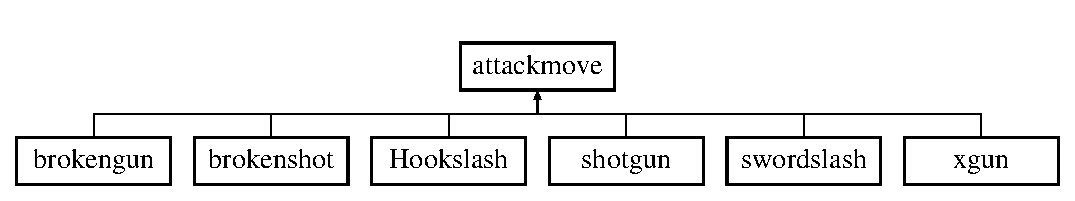
\includegraphics[height=2.000000cm]{classattackmove}
\end{center}
\end{figure}
\subsection*{Public Member Functions}
\begin{DoxyCompactItemize}
\item 
\hypertarget{classattackmove_aeef16b72f9b3b146208a9db33e328b38}{{\bfseries attackmove} (int dam)}\label{classattackmove_aeef16b72f9b3b146208a9db33e328b38}

\item 
\hypertarget{classattackmove_aa971a4aef1cfb1c2ef54301e67e620a6}{int {\bfseries get\-Dam} ()}\label{classattackmove_aa971a4aef1cfb1c2ef54301e67e620a6}

\item 
\hypertarget{classattackmove_a103d4b29b142a466d564de825cf21458}{void {\bfseries set\-Dam} (int dam)}\label{classattackmove_a103d4b29b142a466d564de825cf21458}

\item 
virtual void \hyperlink{classattackmove_a80a498f0903dbe791bb1e0faacb54870}{do\-Attack} (int hpanel, \hyperlink{class_enemy}{Enemy} $\ast$Enemies\mbox{[}3\mbox{]}, \hyperlink{classanim_items}{anim\-Items} $\ast$anim)
\begin{DoxyCompactList}\small\item\em \hyperlink{classattackmove_a80a498f0903dbe791bb1e0faacb54870}{attackmove\-::do\-Attack} does it's attack, implemented for all enemies \end{DoxyCompactList}\item 
virtual Q\-String \hyperlink{classattackmove_ada49eedf4b893372c576edd48fe73161}{get\-String} ()
\begin{DoxyCompactList}\small\item\em \hyperlink{classattackmove_ada49eedf4b893372c576edd48fe73161}{attackmove\-::get\-String} \end{DoxyCompactList}\item 
virtual Q\-Image \hyperlink{classattackmove_aca59a2343b7a6c195d300dda5c8d952d}{get\-Image} ()
\begin{DoxyCompactList}\small\item\em \hyperlink{classattackmove_aca59a2343b7a6c195d300dda5c8d952d}{attackmove\-::get\-Image} \end{DoxyCompactList}\item 
virtual void \hyperlink{classattackmove_a0ff82349551bd72f4d57b3367bb318fa}{get\-Hover} (int hpanel, \hyperlink{class_enemy}{Enemy} $\ast$Enemies\mbox{[}3\mbox{]}, \hyperlink{classanim_items}{anim\-Items} $\ast$anim)
\begin{DoxyCompactList}\small\item\em \hyperlink{classattackmove_a0ff82349551bd72f4d57b3367bb318fa}{attackmove\-::get\-Hover} \end{DoxyCompactList}\end{DoxyCompactItemize}
\subsection*{Protected Attributes}
\begin{DoxyCompactItemize}
\item 
\hypertarget{classattackmove_abeaa53553d9b169032ac273ef2ea7b67}{int {\bfseries damage}}\label{classattackmove_abeaa53553d9b169032ac273ef2ea7b67}

\end{DoxyCompactItemize}


\subsection{Member Function Documentation}
\hypertarget{classattackmove_a80a498f0903dbe791bb1e0faacb54870}{\index{attackmove@{attackmove}!do\-Attack@{do\-Attack}}
\index{do\-Attack@{do\-Attack}!attackmove@{attackmove}}
\subsubsection[{do\-Attack}]{\setlength{\rightskip}{0pt plus 5cm}void attackmove\-::do\-Attack (
\begin{DoxyParamCaption}
\item[{int}]{hpanel, }
\item[{{\bf Enemy} $\ast$}]{Enemies\mbox{[}3\mbox{]}, }
\item[{{\bf anim\-Items} $\ast$}]{anim}
\end{DoxyParamCaption}
)\hspace{0.3cm}{\ttfamily [virtual]}}}\label{classattackmove_a80a498f0903dbe791bb1e0faacb54870}


\hyperlink{classattackmove_a80a498f0903dbe791bb1e0faacb54870}{attackmove\-::do\-Attack} does it's attack, implemented for all enemies 


\begin{DoxyParams}{Parameters}
{\em hpanel,hero's} & panel \\
\hline
{\em Enemies,enemies} & array \\
\hline
{\em anim} & hit animation grid \\
\hline
\end{DoxyParams}
\hypertarget{classattackmove_a0ff82349551bd72f4d57b3367bb318fa}{\index{attackmove@{attackmove}!get\-Hover@{get\-Hover}}
\index{get\-Hover@{get\-Hover}!attackmove@{attackmove}}
\subsubsection[{get\-Hover}]{\setlength{\rightskip}{0pt plus 5cm}void attackmove\-::get\-Hover (
\begin{DoxyParamCaption}
\item[{int}]{hpanel, }
\item[{{\bf Enemy} $\ast$}]{Enemies\mbox{[}3\mbox{]}, }
\item[{{\bf anim\-Items} $\ast$}]{anim}
\end{DoxyParamCaption}
)\hspace{0.3cm}{\ttfamily [virtual]}}}\label{classattackmove_a0ff82349551bd72f4d57b3367bb318fa}


\hyperlink{classattackmove_a0ff82349551bd72f4d57b3367bb318fa}{attackmove\-::get\-Hover} 


\begin{DoxyParams}{Parameters}
{\em hpanel} & \\
\hline
{\em Enemies} & \\
\hline
{\em anim} & \\
\hline
\end{DoxyParams}


Reimplemented in \hyperlink{classshotgun_a8334202fd30d71432db7e58fca7a462e}{shotgun}, \hyperlink{classbrokengun_ab2250f29c2057006662e77d7f70796d2}{brokengun}, \hyperlink{classbrokenshot_a1d9aaa51c4a27d8bb68a8f0678430d3a}{brokenshot}, \hyperlink{class_hookslash_ab6a6ca9582c4d8dad26b481292bca6a0}{Hookslash}, and \hyperlink{classswordslash_af40c617c0463f788bda02fe5e8109511}{swordslash}.

\hypertarget{classattackmove_aca59a2343b7a6c195d300dda5c8d952d}{\index{attackmove@{attackmove}!get\-Image@{get\-Image}}
\index{get\-Image@{get\-Image}!attackmove@{attackmove}}
\subsubsection[{get\-Image}]{\setlength{\rightskip}{0pt plus 5cm}Q\-Image attackmove\-::get\-Image (
\begin{DoxyParamCaption}
{}
\end{DoxyParamCaption}
)\hspace{0.3cm}{\ttfamily [virtual]}}}\label{classattackmove_aca59a2343b7a6c195d300dda5c8d952d}


\hyperlink{classattackmove_aca59a2343b7a6c195d300dda5c8d952d}{attackmove\-::get\-Image} 

\begin{DoxyReturn}{Returns}

\end{DoxyReturn}


Reimplemented in \hyperlink{classshotgun_a1336af80f8d3f7d19ac954f2e616a1b0}{shotgun}, \hyperlink{classbrokengun_aceb704b315cbac5e23093637a9b3c0c0}{brokengun}, \hyperlink{classbrokenshot_ab5a534dcbeb99a57362e22bd11598a27}{brokenshot}, \hyperlink{class_hookslash_a65c6e01ac90d1f01139dd08b93aeaa0a}{Hookslash}, \hyperlink{classswordslash_a25cbfa2df6b5718a299eed09cf716822}{swordslash}, and \hyperlink{classxgun_adf5511bd6ed5dfb184a8a3b6b757608a}{xgun}.

\hypertarget{classattackmove_ada49eedf4b893372c576edd48fe73161}{\index{attackmove@{attackmove}!get\-String@{get\-String}}
\index{get\-String@{get\-String}!attackmove@{attackmove}}
\subsubsection[{get\-String}]{\setlength{\rightskip}{0pt plus 5cm}Q\-String attackmove\-::get\-String (
\begin{DoxyParamCaption}
{}
\end{DoxyParamCaption}
)\hspace{0.3cm}{\ttfamily [virtual]}}}\label{classattackmove_ada49eedf4b893372c576edd48fe73161}


\hyperlink{classattackmove_ada49eedf4b893372c576edd48fe73161}{attackmove\-::get\-String} 

\begin{DoxyReturn}{Returns}
string of name, implemented in all inheritences includes damage 
\end{DoxyReturn}


Reimplemented in \hyperlink{classshotgun_a856fa8335ee3c2bb8603e83aa5629e5c}{shotgun}, \hyperlink{classbrokengun_af525de1fc249ff4fadec008b367881e9}{brokengun}, \hyperlink{classbrokenshot_a4834069bb57b3bb17a4816888cc83e43}{brokenshot}, \hyperlink{class_hookslash_aaf31aabb624b138d98f3c94fe1c37fcc}{Hookslash}, \hyperlink{classswordslash_ac58a7e3b969bb957548c55bdfd6a0b05}{swordslash}, and \hyperlink{classxgun_a8d091859d655ff1703630ba7dd88a358}{xgun}.



The documentation for this class was generated from the following files\-:\begin{DoxyCompactItemize}
\item 
attackmove.\-h\item 
attackmove.\-cpp\end{DoxyCompactItemize}

\hypertarget{class_back_from_end}{\section{Back\-From\-End Class Reference}
\label{class_back_from_end}\index{Back\-From\-End@{Back\-From\-End}}
}
Inheritance diagram for Back\-From\-End\-:\begin{figure}[H]
\begin{center}
\leavevmode
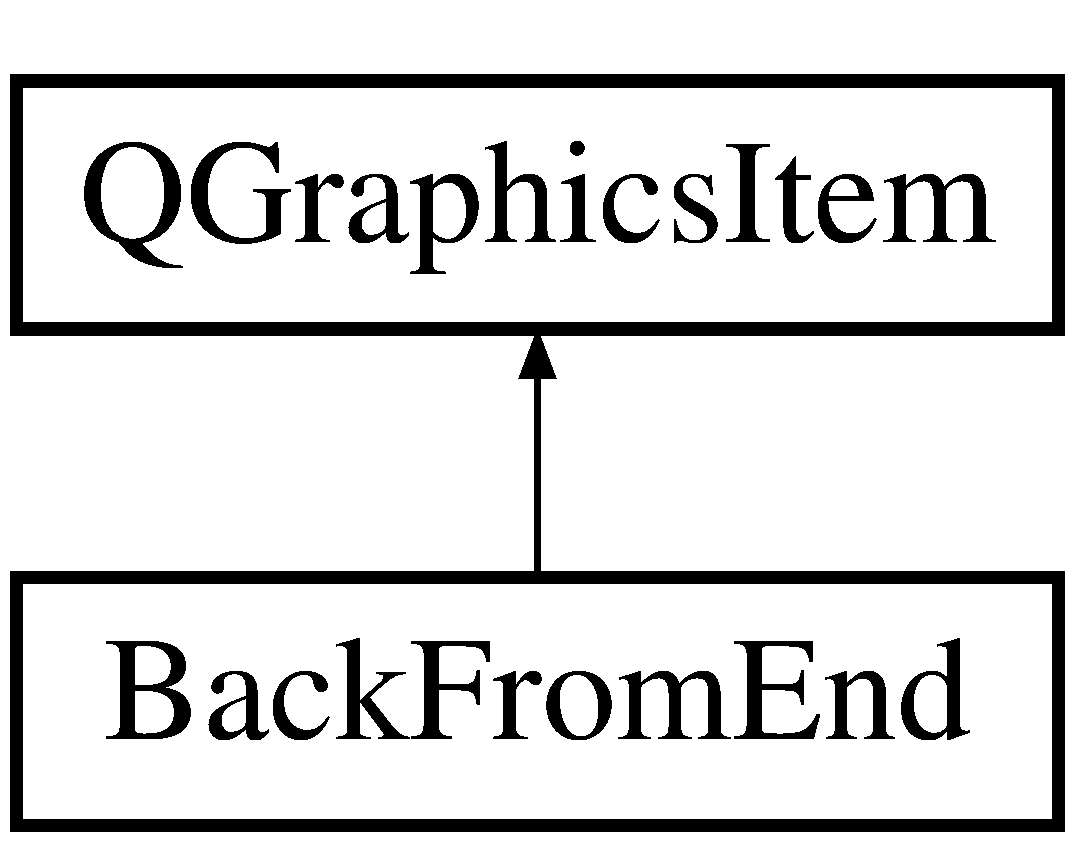
\includegraphics[height=2.000000cm]{class_back_from_end}
\end{center}
\end{figure}
\subsection*{Public Member Functions}
\begin{DoxyCompactItemize}
\item 
\hyperlink{class_back_from_end_a64a9aa1b79a4b24dc8f770119380bcf0}{Back\-From\-End} (Q\-Graphics\-Item $\ast$parent=N\-U\-L\-L)
\begin{DoxyCompactList}\small\item\em Constructor that does nothing. \end{DoxyCompactList}\item 
void \hyperlink{class_back_from_end_a69972808b1eacfa0fbe2021c8db14a54}{paint} (Q\-Painter $\ast$painter, const Q\-Style\-Option\-Graphics\-Item $\ast$option, Q\-Widget $\ast$widget)
\begin{DoxyCompactList}\small\item\em Paints the object onto the screen. \end{DoxyCompactList}\item 
\hypertarget{class_back_from_end_ad61e8913026f3741a5b2918e84ce1890}{\hyperlink{class_back_from_end_ad61e8913026f3741a5b2918e84ce1890}{$\sim$\-Back\-From\-End} ()}\label{class_back_from_end_ad61e8913026f3741a5b2918e84ce1890}

\begin{DoxyCompactList}\small\item\em hides the item when destructor is called. \end{DoxyCompactList}\end{DoxyCompactItemize}
\subsection*{Protected Member Functions}
\begin{DoxyCompactItemize}
\item 
Q\-Rect\-F \hyperlink{class_back_from_end_a30bf2628ade3dd6e43eb23ba235327db}{bounding\-Rect} () const 
\begin{DoxyCompactList}\small\item\em sets the coordinates to the object. \end{DoxyCompactList}\end{DoxyCompactItemize}


\subsection{Constructor \& Destructor Documentation}
\hypertarget{class_back_from_end_a64a9aa1b79a4b24dc8f770119380bcf0}{\index{Back\-From\-End@{Back\-From\-End}!Back\-From\-End@{Back\-From\-End}}
\index{Back\-From\-End@{Back\-From\-End}!BackFromEnd@{Back\-From\-End}}
\subsubsection[{Back\-From\-End}]{\setlength{\rightskip}{0pt plus 5cm}Back\-From\-End\-::\-Back\-From\-End (
\begin{DoxyParamCaption}
\item[{Q\-Graphics\-Item $\ast$}]{parent = {\ttfamily NULL}}
\end{DoxyParamCaption}
)}}\label{class_back_from_end_a64a9aa1b79a4b24dc8f770119380bcf0}


Constructor that does nothing. 


\begin{DoxyParams}{Parameters}
{\em parent} & \\
\hline
\end{DoxyParams}


\subsection{Member Function Documentation}
\hypertarget{class_back_from_end_a30bf2628ade3dd6e43eb23ba235327db}{\index{Back\-From\-End@{Back\-From\-End}!bounding\-Rect@{bounding\-Rect}}
\index{bounding\-Rect@{bounding\-Rect}!BackFromEnd@{Back\-From\-End}}
\subsubsection[{bounding\-Rect}]{\setlength{\rightskip}{0pt plus 5cm}Q\-Rect\-F Back\-From\-End\-::bounding\-Rect (
\begin{DoxyParamCaption}
{}
\end{DoxyParamCaption}
) const\hspace{0.3cm}{\ttfamily [protected]}}}\label{class_back_from_end_a30bf2628ade3dd6e43eb23ba235327db}


sets the coordinates to the object. 

\begin{DoxyReturn}{Returns}

\end{DoxyReturn}
\hypertarget{class_back_from_end_a69972808b1eacfa0fbe2021c8db14a54}{\index{Back\-From\-End@{Back\-From\-End}!paint@{paint}}
\index{paint@{paint}!BackFromEnd@{Back\-From\-End}}
\subsubsection[{paint}]{\setlength{\rightskip}{0pt plus 5cm}void Back\-From\-End\-::paint (
\begin{DoxyParamCaption}
\item[{Q\-Painter $\ast$}]{painter, }
\item[{const Q\-Style\-Option\-Graphics\-Item $\ast$}]{option, }
\item[{Q\-Widget $\ast$}]{widget}
\end{DoxyParamCaption}
)}}\label{class_back_from_end_a69972808b1eacfa0fbe2021c8db14a54}


Paints the object onto the screen. 


\begin{DoxyParams}{Parameters}
{\em painter,is} & a pointer to the painter \\
\hline
{\em option,a} & non used paramaters \\
\hline
{\em widget,another} & non used paramter for our code. \\
\hline
\end{DoxyParams}


The documentation for this class was generated from the following files\-:\begin{DoxyCompactItemize}
\item 
backfromend.\-h\item 
backfromend.\-cpp\end{DoxyCompactItemize}

\hypertarget{class_back_from_in_store}{\section{Back\-From\-In\-Store Class Reference}
\label{class_back_from_in_store}\index{Back\-From\-In\-Store@{Back\-From\-In\-Store}}
}
Inheritance diagram for Back\-From\-In\-Store\-:\begin{figure}[H]
\begin{center}
\leavevmode
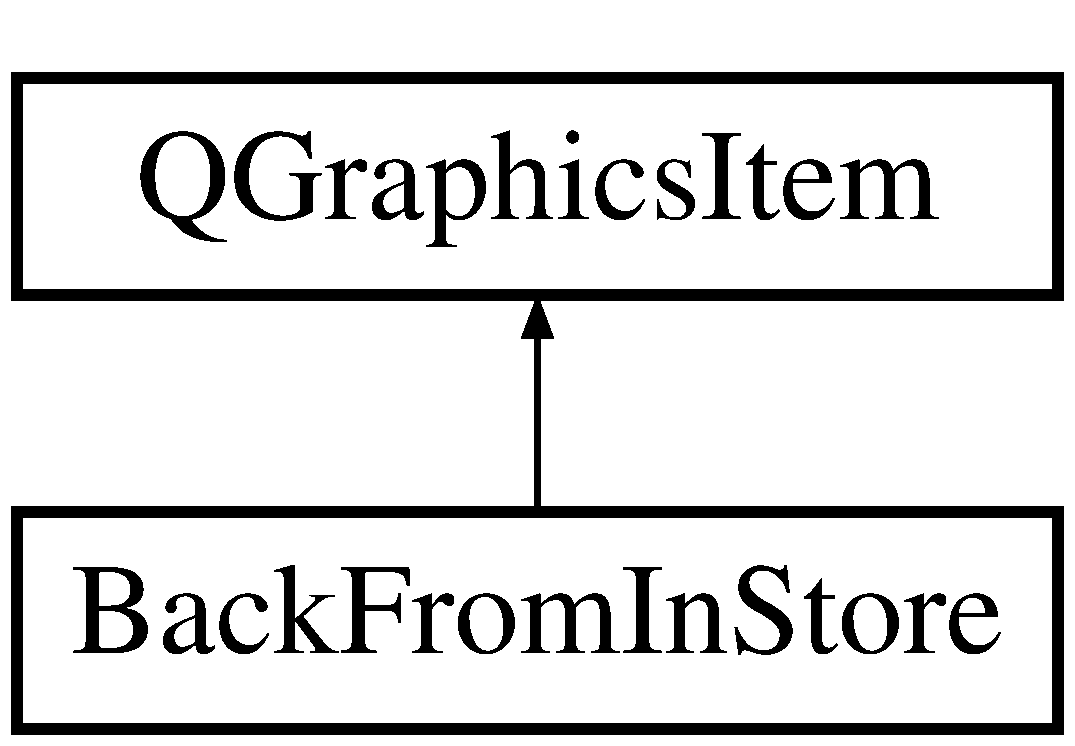
\includegraphics[height=2.000000cm]{class_back_from_in_store}
\end{center}
\end{figure}
\subsection*{Public Member Functions}
\begin{DoxyCompactItemize}
\item 
\hyperlink{class_back_from_in_store_a3bbe96f2b704d66dd72193a8c9157162}{Back\-From\-In\-Store} (Q\-Graphics\-Item $\ast$parent=N\-U\-L\-L)
\begin{DoxyCompactList}\small\item\em Constructor for the item. \end{DoxyCompactList}\item 
void \hyperlink{class_back_from_in_store_a6f36fa5bfe7d155b6d9d0899615430dc}{paint} (Q\-Painter $\ast$painter, const Q\-Style\-Option\-Graphics\-Item $\ast$option, Q\-Widget $\ast$widget)
\begin{DoxyCompactList}\small\item\em Paint item that paints the item. \end{DoxyCompactList}\item 
\hypertarget{class_back_from_in_store_a09fc63157033073cee58a3044113d224}{\hyperlink{class_back_from_in_store_a09fc63157033073cee58a3044113d224}{$\sim$\-Back\-From\-In\-Store} ()}\label{class_back_from_in_store_a09fc63157033073cee58a3044113d224}

\begin{DoxyCompactList}\small\item\em destructor hides the item if called. \end{DoxyCompactList}\end{DoxyCompactItemize}
\subsection*{Protected Member Functions}
\begin{DoxyCompactItemize}
\item 
Q\-Rect\-F \hyperlink{class_back_from_in_store_a70ccb3817000b00e7ccbcffef90bcee2}{bounding\-Rect} () const 
\begin{DoxyCompactList}\small\item\em The bounding rect for the item. \end{DoxyCompactList}\end{DoxyCompactItemize}


\subsection{Constructor \& Destructor Documentation}
\hypertarget{class_back_from_in_store_a3bbe96f2b704d66dd72193a8c9157162}{\index{Back\-From\-In\-Store@{Back\-From\-In\-Store}!Back\-From\-In\-Store@{Back\-From\-In\-Store}}
\index{Back\-From\-In\-Store@{Back\-From\-In\-Store}!BackFromInStore@{Back\-From\-In\-Store}}
\subsubsection[{Back\-From\-In\-Store}]{\setlength{\rightskip}{0pt plus 5cm}Back\-From\-In\-Store\-::\-Back\-From\-In\-Store (
\begin{DoxyParamCaption}
\item[{Q\-Graphics\-Item $\ast$}]{parent = {\ttfamily NULL}}
\end{DoxyParamCaption}
)}}\label{class_back_from_in_store_a3bbe96f2b704d66dd72193a8c9157162}


Constructor for the item. 


\begin{DoxyParams}{Parameters}
{\em parent} & \\
\hline
\end{DoxyParams}


\subsection{Member Function Documentation}
\hypertarget{class_back_from_in_store_a70ccb3817000b00e7ccbcffef90bcee2}{\index{Back\-From\-In\-Store@{Back\-From\-In\-Store}!bounding\-Rect@{bounding\-Rect}}
\index{bounding\-Rect@{bounding\-Rect}!BackFromInStore@{Back\-From\-In\-Store}}
\subsubsection[{bounding\-Rect}]{\setlength{\rightskip}{0pt plus 5cm}Q\-Rect\-F Back\-From\-In\-Store\-::bounding\-Rect (
\begin{DoxyParamCaption}
{}
\end{DoxyParamCaption}
) const\hspace{0.3cm}{\ttfamily [protected]}}}\label{class_back_from_in_store_a70ccb3817000b00e7ccbcffef90bcee2}


The bounding rect for the item. 

\begin{DoxyReturn}{Returns}
returns a Q\-Rect bounding rect 
\end{DoxyReturn}
\hypertarget{class_back_from_in_store_a6f36fa5bfe7d155b6d9d0899615430dc}{\index{Back\-From\-In\-Store@{Back\-From\-In\-Store}!paint@{paint}}
\index{paint@{paint}!BackFromInStore@{Back\-From\-In\-Store}}
\subsubsection[{paint}]{\setlength{\rightskip}{0pt plus 5cm}void Back\-From\-In\-Store\-::paint (
\begin{DoxyParamCaption}
\item[{Q\-Painter $\ast$}]{painter, }
\item[{const Q\-Style\-Option\-Graphics\-Item $\ast$}]{option, }
\item[{Q\-Widget $\ast$}]{widget}
\end{DoxyParamCaption}
)}}\label{class_back_from_in_store_a6f36fa5bfe7d155b6d9d0899615430dc}


Paint item that paints the item. 


\begin{DoxyParams}{Parameters}
{\em painter,used} & to set the brush in this case. \\
\hline
{\em option} & \\
\hline
{\em widget} & \\
\hline
\end{DoxyParams}


The documentation for this class was generated from the following files\-:\begin{DoxyCompactItemize}
\item 
backfrominstore.\-h\item 
backfrominstore.\-cpp\end{DoxyCompactItemize}

\hypertarget{class_back_from_store}{\section{Back\-From\-Store Class Reference}
\label{class_back_from_store}\index{Back\-From\-Store@{Back\-From\-Store}}
}
Inheritance diagram for Back\-From\-Store\-:\begin{figure}[H]
\begin{center}
\leavevmode
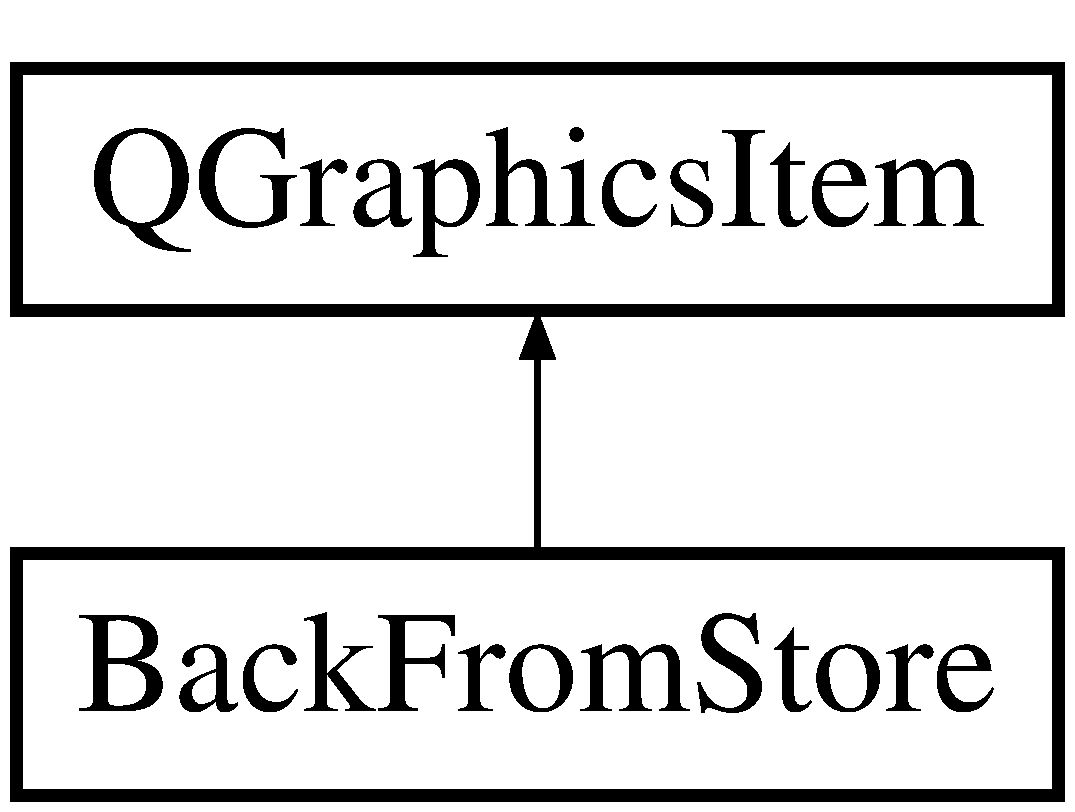
\includegraphics[height=2.000000cm]{class_back_from_store}
\end{center}
\end{figure}
\subsection*{Public Member Functions}
\begin{DoxyCompactItemize}
\item 
\hyperlink{class_back_from_store_a9e92e57e75e179d5929e13d7786bbae6}{Back\-From\-Store} (Q\-Graphics\-Item $\ast$parent=N\-U\-L\-L)
\begin{DoxyCompactList}\small\item\em Constructor for the item. \end{DoxyCompactList}\item 
void \hyperlink{class_back_from_store_a9bd0ae2bf7216a99e030a199df7b1582}{paint} (Q\-Painter $\ast$painter, const Q\-Style\-Option\-Graphics\-Item $\ast$option, Q\-Widget $\ast$widget)
\begin{DoxyCompactList}\small\item\em Paints the item, which will be used in the scene. \end{DoxyCompactList}\item 
\hypertarget{class_back_from_store_ad9766708c35f543f9b3ec96e0f96b75b}{\hyperlink{class_back_from_store_ad9766708c35f543f9b3ec96e0f96b75b}{$\sim$\-Back\-From\-Store} ()}\label{class_back_from_store_ad9766708c35f543f9b3ec96e0f96b75b}

\begin{DoxyCompactList}\small\item\em destructor to hide the item \end{DoxyCompactList}\end{DoxyCompactItemize}
\subsection*{Protected Member Functions}
\begin{DoxyCompactItemize}
\item 
Q\-Rect\-F \hyperlink{class_back_from_store_a2016b61256fee7cbd4e1590737cde48e}{bounding\-Rect} () const 
\begin{DoxyCompactList}\small\item\em returns a bounding rect and sets the bouding rect for the item. \end{DoxyCompactList}\end{DoxyCompactItemize}


\subsection{Constructor \& Destructor Documentation}
\hypertarget{class_back_from_store_a9e92e57e75e179d5929e13d7786bbae6}{\index{Back\-From\-Store@{Back\-From\-Store}!Back\-From\-Store@{Back\-From\-Store}}
\index{Back\-From\-Store@{Back\-From\-Store}!BackFromStore@{Back\-From\-Store}}
\subsubsection[{Back\-From\-Store}]{\setlength{\rightskip}{0pt plus 5cm}Back\-From\-Store\-::\-Back\-From\-Store (
\begin{DoxyParamCaption}
\item[{Q\-Graphics\-Item $\ast$}]{parent = {\ttfamily NULL}}
\end{DoxyParamCaption}
)}}\label{class_back_from_store_a9e92e57e75e179d5929e13d7786bbae6}


Constructor for the item. 


\begin{DoxyParams}{Parameters}
{\em parent} & \\
\hline
\end{DoxyParams}


\subsection{Member Function Documentation}
\hypertarget{class_back_from_store_a2016b61256fee7cbd4e1590737cde48e}{\index{Back\-From\-Store@{Back\-From\-Store}!bounding\-Rect@{bounding\-Rect}}
\index{bounding\-Rect@{bounding\-Rect}!BackFromStore@{Back\-From\-Store}}
\subsubsection[{bounding\-Rect}]{\setlength{\rightskip}{0pt plus 5cm}Q\-Rect\-F Back\-From\-Store\-::bounding\-Rect (
\begin{DoxyParamCaption}
{}
\end{DoxyParamCaption}
) const\hspace{0.3cm}{\ttfamily [protected]}}}\label{class_back_from_store_a2016b61256fee7cbd4e1590737cde48e}


returns a bounding rect and sets the bouding rect for the item. 

\begin{DoxyReturn}{Returns}

\end{DoxyReturn}
\hypertarget{class_back_from_store_a9bd0ae2bf7216a99e030a199df7b1582}{\index{Back\-From\-Store@{Back\-From\-Store}!paint@{paint}}
\index{paint@{paint}!BackFromStore@{Back\-From\-Store}}
\subsubsection[{paint}]{\setlength{\rightskip}{0pt plus 5cm}void Back\-From\-Store\-::paint (
\begin{DoxyParamCaption}
\item[{Q\-Painter $\ast$}]{painter, }
\item[{const Q\-Style\-Option\-Graphics\-Item $\ast$}]{option, }
\item[{Q\-Widget $\ast$}]{widget}
\end{DoxyParamCaption}
)}}\label{class_back_from_store_a9bd0ae2bf7216a99e030a199df7b1582}


Paints the item, which will be used in the scene. 


\begin{DoxyParams}{Parameters}
{\em painter,a} & pointer to the painter that paints the item. \\
\hline
{\em option} & \\
\hline
{\em widget} & \\
\hline
\end{DoxyParams}


The documentation for this class was generated from the following files\-:\begin{DoxyCompactItemize}
\item 
backfromstore.\-h\item 
backfromstore.\-cpp\end{DoxyCompactItemize}

\hypertarget{class_ui_1_1_battle_pause}{\section{Ui\-:\-:Battle\-Pause Class Reference}
\label{class_ui_1_1_battle_pause}\index{Ui\-::\-Battle\-Pause@{Ui\-::\-Battle\-Pause}}
}
Inheritance diagram for Ui\-:\-:Battle\-Pause\-:\begin{figure}[H]
\begin{center}
\leavevmode
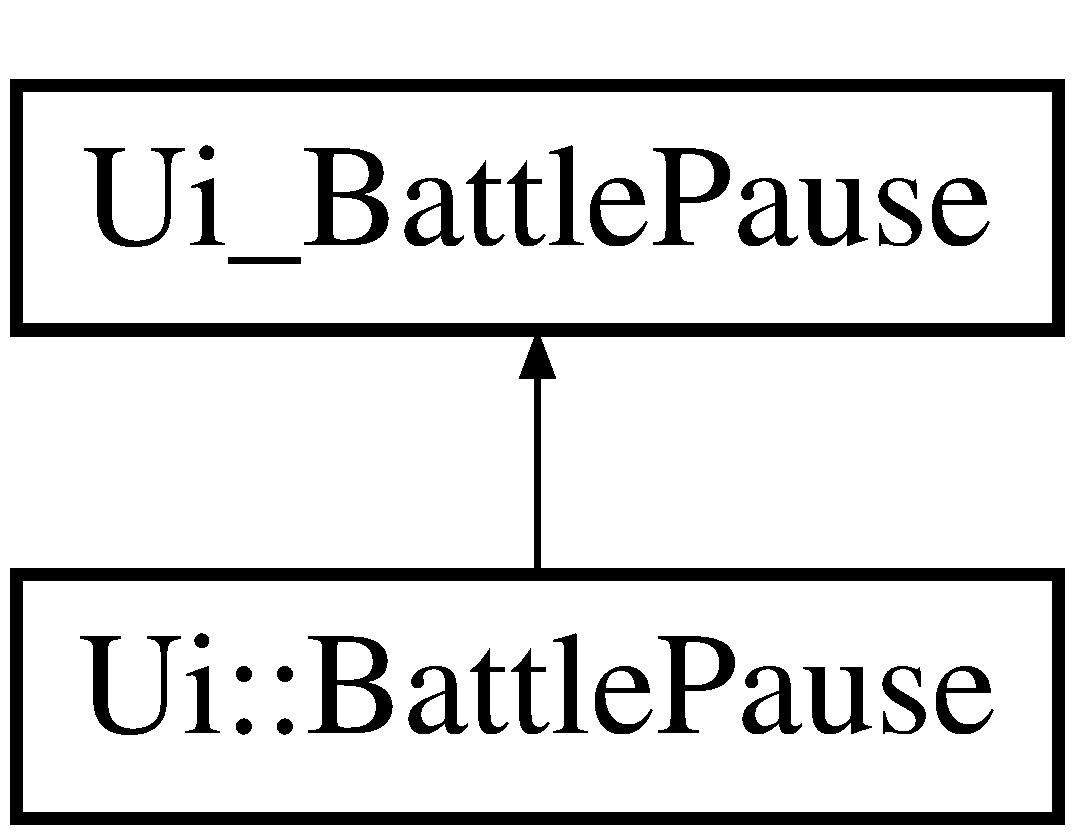
\includegraphics[height=2.000000cm]{class_ui_1_1_battle_pause}
\end{center}
\end{figure}
\subsection*{Additional Inherited Members}


The documentation for this class was generated from the following file\-:\begin{DoxyCompactItemize}
\item 
ui\-\_\-battlepause.\-h\end{DoxyCompactItemize}

\hypertarget{class_bomber}{\section{Bomber Class Reference}
\label{class_bomber}\index{Bomber@{Bomber}}
}
Inheritance diagram for Bomber\-:\begin{figure}[H]
\begin{center}
\leavevmode
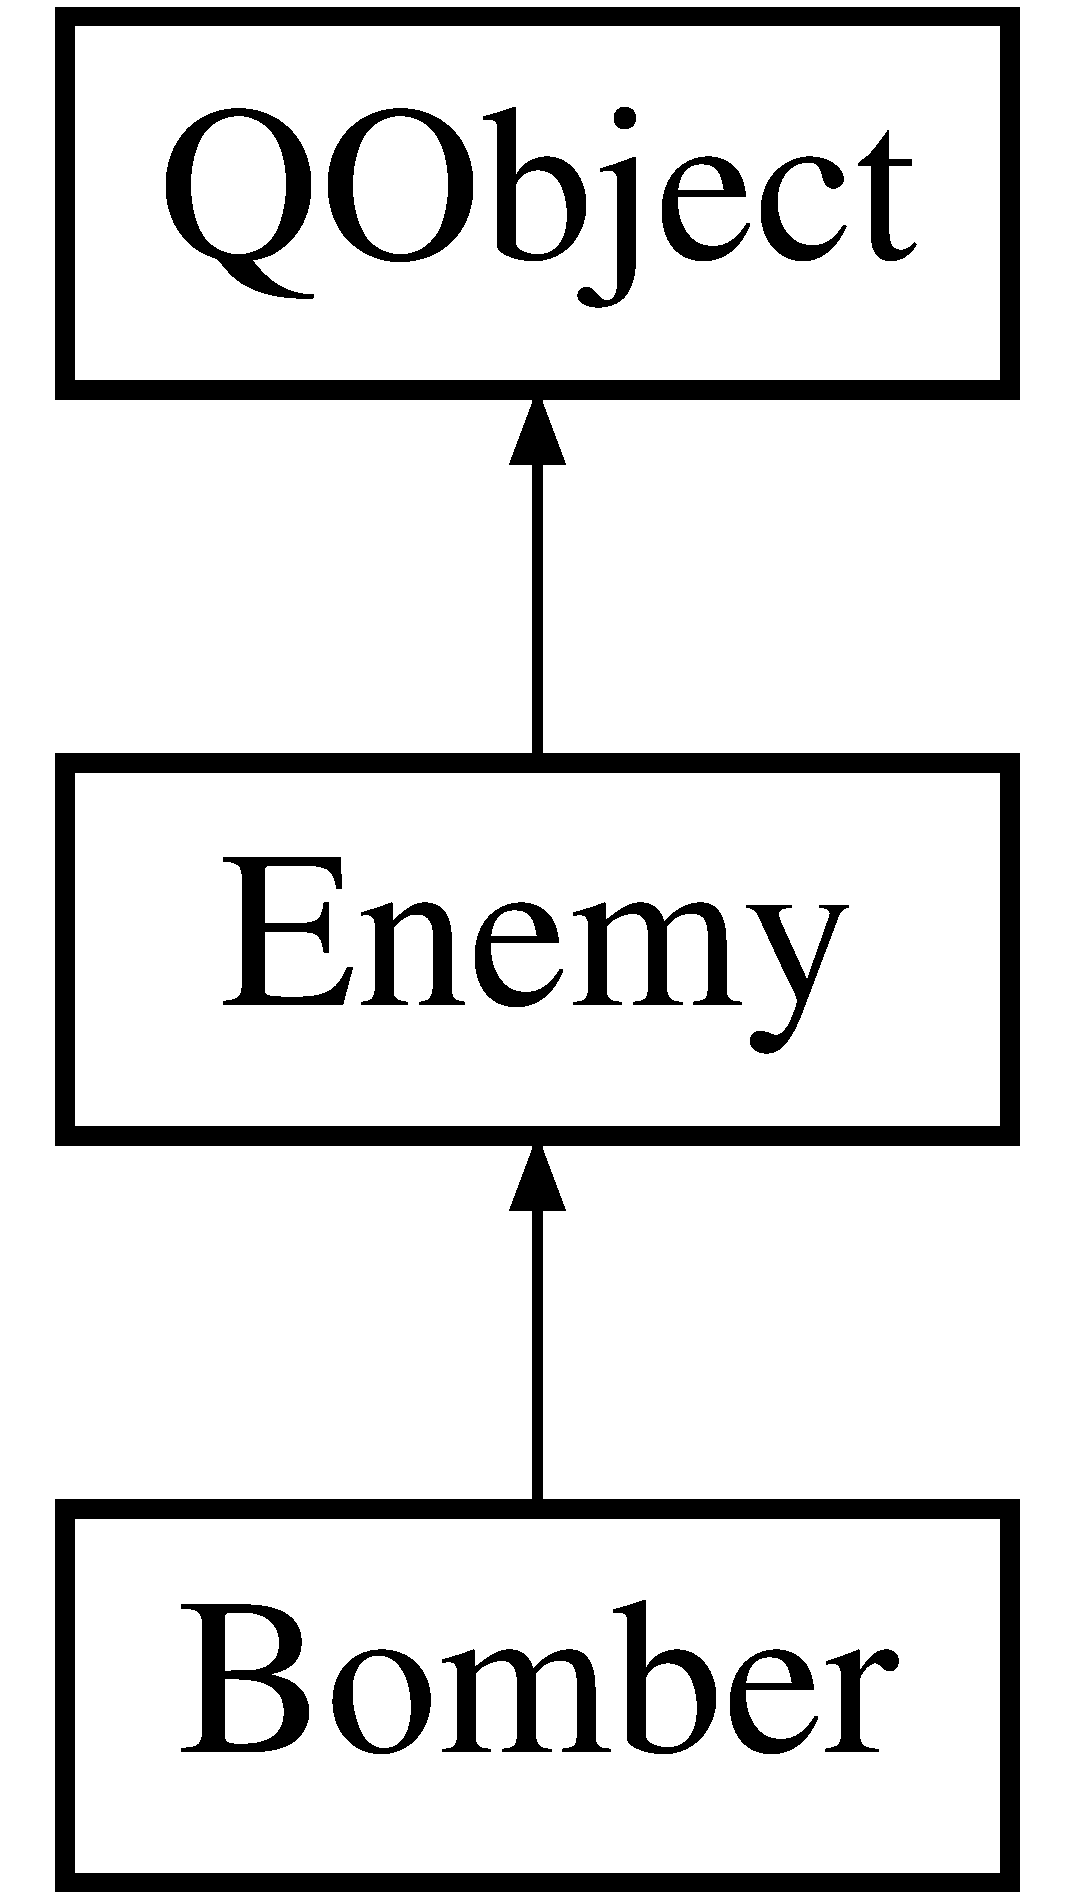
\includegraphics[height=3.000000cm]{class_bomber}
\end{center}
\end{figure}
\subsection*{Public Member Functions}
\begin{DoxyCompactItemize}
\item 
\hypertarget{class_bomber_a69a81ac540c1330e0e6469d236ec5914}{{\bfseries Bomber} (int clev, int cx, int cy)}\label{class_bomber_a69a81ac540c1330e0e6469d236ec5914}

\item 
virtual void \hyperlink{class_bomber_ac0f488834e2abdab290699d6efa6e72e}{do\-Turn} (\hyperlink{class_character}{Character} $\ast$Hero)
\begin{DoxyCompactList}\small\item\em \hyperlink{class_enemy_a56e4b9b07e8cd2a4e5ecfa8ff5b9265a}{Enemy\-::do\-Turn} based on hero's panel, does it's move. \end{DoxyCompactList}\item 
\hypertarget{class_bomber_a1ea183ca52092dc27c08f6595072b3a5}{void {\bfseries switch\-Side} ()}\label{class_bomber_a1ea183ca52092dc27c08f6595072b3a5}

\item 
\hypertarget{class_bomber_a500004b8c74a11109bc8174340f3c72d}{void {\bfseries drop\-Bomb} (\hyperlink{class_character}{Character} $\ast$Hero)}\label{class_bomber_a500004b8c74a11109bc8174340f3c72d}

\item 
\hypertarget{class_bomber_af3d20f9c5832eafe7530a22d04294951}{int {\bfseries get\-Ctr} ()}\label{class_bomber_af3d20f9c5832eafe7530a22d04294951}

\item 
\hypertarget{class_bomber_a3b181f6557c19d65adfddb9226a4edfb}{virtual Q\-Image {\bfseries get\-Pic} ()}\label{class_bomber_a3b181f6557c19d65adfddb9226a4edfb}

\item 
virtual void \hyperlink{class_bomber_aa75d9256efa7f2996a599deb3db83f90}{draw\-Self} (Q\-Painter $\ast$g, int gx, int gy)
\begin{DoxyCompactList}\small\item\em \hyperlink{class_enemy_a3251244e8e7ac657687d6be5a8da71bb}{Enemy\-::draw\-Self} draws itself using painter, includes title and hp. \end{DoxyCompactList}\end{DoxyCompactItemize}
\subsection*{Additional Inherited Members}


\subsection{Member Function Documentation}
\hypertarget{class_bomber_ac0f488834e2abdab290699d6efa6e72e}{\index{Bomber@{Bomber}!do\-Turn@{do\-Turn}}
\index{do\-Turn@{do\-Turn}!Bomber@{Bomber}}
\subsubsection[{do\-Turn}]{\setlength{\rightskip}{0pt plus 5cm}void Bomber\-::do\-Turn (
\begin{DoxyParamCaption}
\item[{{\bf Character} $\ast$}]{Hero}
\end{DoxyParamCaption}
)\hspace{0.3cm}{\ttfamily [virtual]}}}\label{class_bomber_ac0f488834e2abdab290699d6efa6e72e}


\hyperlink{class_enemy_a56e4b9b07e8cd2a4e5ecfa8ff5b9265a}{Enemy\-::do\-Turn} based on hero's panel, does it's move. 


\begin{DoxyParams}{Parameters}
{\em Hero} & \\
\hline
\end{DoxyParams}


Reimplemented from \hyperlink{class_enemy_a56e4b9b07e8cd2a4e5ecfa8ff5b9265a}{Enemy}.

\hypertarget{class_bomber_aa75d9256efa7f2996a599deb3db83f90}{\index{Bomber@{Bomber}!draw\-Self@{draw\-Self}}
\index{draw\-Self@{draw\-Self}!Bomber@{Bomber}}
\subsubsection[{draw\-Self}]{\setlength{\rightskip}{0pt plus 5cm}void Bomber\-::draw\-Self (
\begin{DoxyParamCaption}
\item[{Q\-Painter $\ast$}]{g, }
\item[{int}]{gx, }
\item[{int}]{gy}
\end{DoxyParamCaption}
)\hspace{0.3cm}{\ttfamily [virtual]}}}\label{class_bomber_aa75d9256efa7f2996a599deb3db83f90}


\hyperlink{class_enemy_a3251244e8e7ac657687d6be5a8da71bb}{Enemy\-::draw\-Self} draws itself using painter, includes title and hp. 


\begin{DoxyParams}{Parameters}
{\em g} & \\
\hline
{\em gx} & \\
\hline
{\em gy} & \\
\hline
\end{DoxyParams}


Reimplemented from \hyperlink{class_enemy_a3251244e8e7ac657687d6be5a8da71bb}{Enemy}.



The documentation for this class was generated from the following files\-:\begin{DoxyCompactItemize}
\item 
bomber.\-h\item 
bomber.\-cpp\end{DoxyCompactItemize}

\hypertarget{classbrokengun}{\section{brokengun Class Reference}
\label{classbrokengun}\index{brokengun@{brokengun}}
}
Inheritance diagram for brokengun\-:\begin{figure}[H]
\begin{center}
\leavevmode
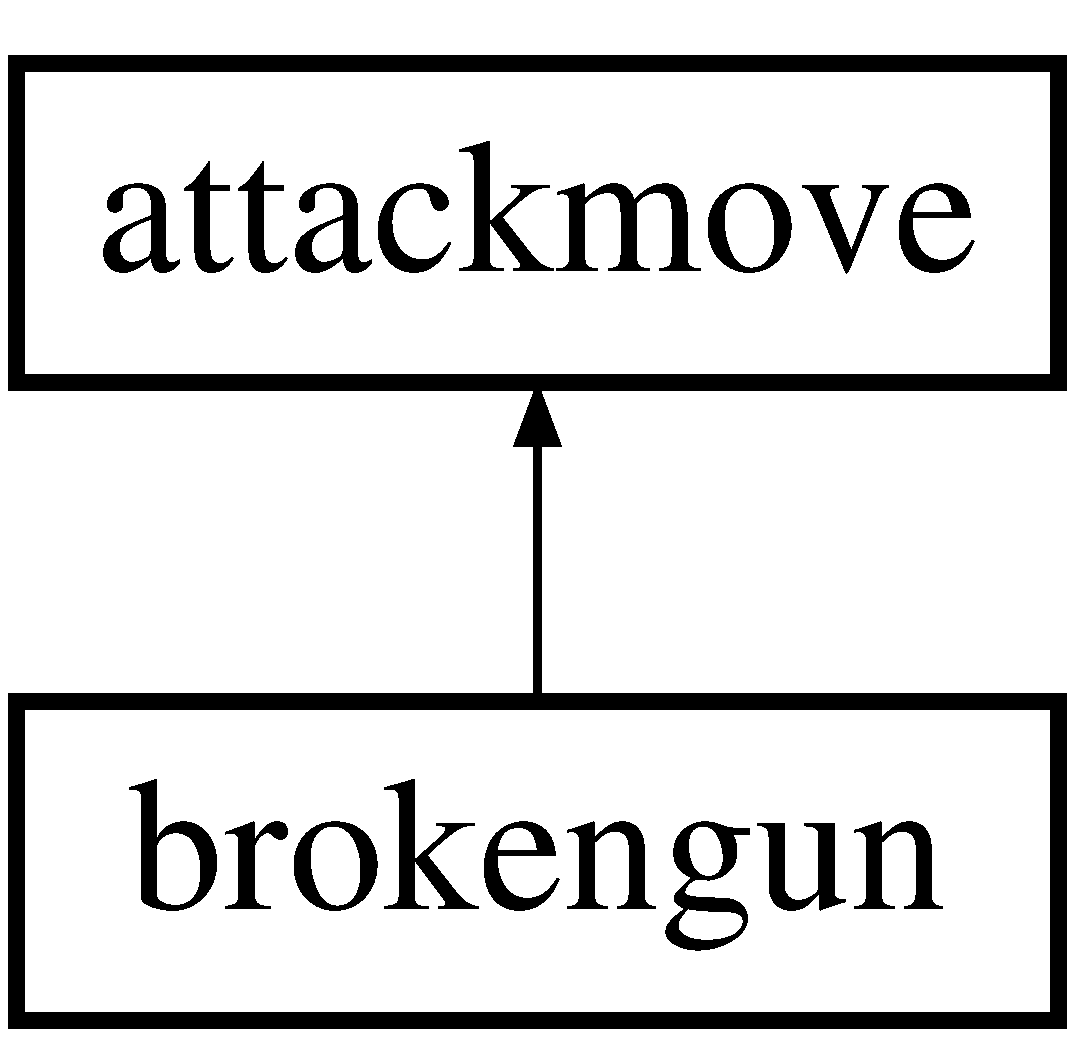
\includegraphics[height=2.000000cm]{classbrokengun}
\end{center}
\end{figure}
\subsection*{Public Member Functions}
\begin{DoxyCompactItemize}
\item 
\hypertarget{classbrokengun_a01e8a685a44e19355ef284c3f172532c}{{\bfseries brokengun} (int dam)}\label{classbrokengun_a01e8a685a44e19355ef284c3f172532c}

\item 
virtual Q\-String \hyperlink{classbrokengun_af525de1fc249ff4fadec008b367881e9}{get\-String} ()
\begin{DoxyCompactList}\small\item\em \hyperlink{classattackmove_ada49eedf4b893372c576edd48fe73161}{attackmove\-::get\-String} \end{DoxyCompactList}\item 
virtual Q\-Image \hyperlink{classbrokengun_aceb704b315cbac5e23093637a9b3c0c0}{get\-Image} ()
\begin{DoxyCompactList}\small\item\em \hyperlink{classattackmove_aca59a2343b7a6c195d300dda5c8d952d}{attackmove\-::get\-Image} \end{DoxyCompactList}\item 
virtual void \hyperlink{classbrokengun_ab2250f29c2057006662e77d7f70796d2}{get\-Hover} (int hpanel, \hyperlink{class_enemy}{Enemy} $\ast$Enemies\mbox{[}3\mbox{]}, \hyperlink{classanim_items}{anim\-Items} $\ast$anim)
\begin{DoxyCompactList}\small\item\em \hyperlink{classattackmove_a0ff82349551bd72f4d57b3367bb318fa}{attackmove\-::get\-Hover} \end{DoxyCompactList}\item 
\hypertarget{classbrokengun_a36f299faa4df56576af55adbff08a9be}{virtual void {\bfseries do\-Attack} (int hpanel, \hyperlink{class_enemy}{Enemy} $\ast$Enemies\mbox{[}$\,$\mbox{]}, \hyperlink{classanim_items}{anim\-Items} $\ast$anim)}\label{classbrokengun_a36f299faa4df56576af55adbff08a9be}

\end{DoxyCompactItemize}
\subsection*{Additional Inherited Members}


\subsection{Member Function Documentation}
\hypertarget{classbrokengun_ab2250f29c2057006662e77d7f70796d2}{\index{brokengun@{brokengun}!get\-Hover@{get\-Hover}}
\index{get\-Hover@{get\-Hover}!brokengun@{brokengun}}
\subsubsection[{get\-Hover}]{\setlength{\rightskip}{0pt plus 5cm}void brokengun\-::get\-Hover (
\begin{DoxyParamCaption}
\item[{int}]{hpanel, }
\item[{{\bf Enemy} $\ast$}]{Enemies\mbox{[}3\mbox{]}, }
\item[{{\bf anim\-Items} $\ast$}]{anim}
\end{DoxyParamCaption}
)\hspace{0.3cm}{\ttfamily [virtual]}}}\label{classbrokengun_ab2250f29c2057006662e77d7f70796d2}


\hyperlink{classattackmove_a0ff82349551bd72f4d57b3367bb318fa}{attackmove\-::get\-Hover} 


\begin{DoxyParams}{Parameters}
{\em hpanel} & \\
\hline
{\em Enemies} & \\
\hline
{\em anim} & \\
\hline
\end{DoxyParams}


Reimplemented from \hyperlink{classattackmove_a0ff82349551bd72f4d57b3367bb318fa}{attackmove}.

\hypertarget{classbrokengun_aceb704b315cbac5e23093637a9b3c0c0}{\index{brokengun@{brokengun}!get\-Image@{get\-Image}}
\index{get\-Image@{get\-Image}!brokengun@{brokengun}}
\subsubsection[{get\-Image}]{\setlength{\rightskip}{0pt plus 5cm}Q\-Image brokengun\-::get\-Image (
\begin{DoxyParamCaption}
{}
\end{DoxyParamCaption}
)\hspace{0.3cm}{\ttfamily [virtual]}}}\label{classbrokengun_aceb704b315cbac5e23093637a9b3c0c0}


\hyperlink{classattackmove_aca59a2343b7a6c195d300dda5c8d952d}{attackmove\-::get\-Image} 

\begin{DoxyReturn}{Returns}

\end{DoxyReturn}


Reimplemented from \hyperlink{classattackmove_aca59a2343b7a6c195d300dda5c8d952d}{attackmove}.

\hypertarget{classbrokengun_af525de1fc249ff4fadec008b367881e9}{\index{brokengun@{brokengun}!get\-String@{get\-String}}
\index{get\-String@{get\-String}!brokengun@{brokengun}}
\subsubsection[{get\-String}]{\setlength{\rightskip}{0pt plus 5cm}Q\-String brokengun\-::get\-String (
\begin{DoxyParamCaption}
{}
\end{DoxyParamCaption}
)\hspace{0.3cm}{\ttfamily [virtual]}}}\label{classbrokengun_af525de1fc249ff4fadec008b367881e9}


\hyperlink{classattackmove_ada49eedf4b893372c576edd48fe73161}{attackmove\-::get\-String} 

\begin{DoxyReturn}{Returns}
string of name, implemented in all inheritences includes damage 
\end{DoxyReturn}


Reimplemented from \hyperlink{classattackmove_ada49eedf4b893372c576edd48fe73161}{attackmove}.



The documentation for this class was generated from the following files\-:\begin{DoxyCompactItemize}
\item 
brokengun.\-h\item 
brokengun.\-cpp\end{DoxyCompactItemize}

\hypertarget{classbrokenshot}{\section{brokenshot Class Reference}
\label{classbrokenshot}\index{brokenshot@{brokenshot}}
}
Inheritance diagram for brokenshot\-:\begin{figure}[H]
\begin{center}
\leavevmode
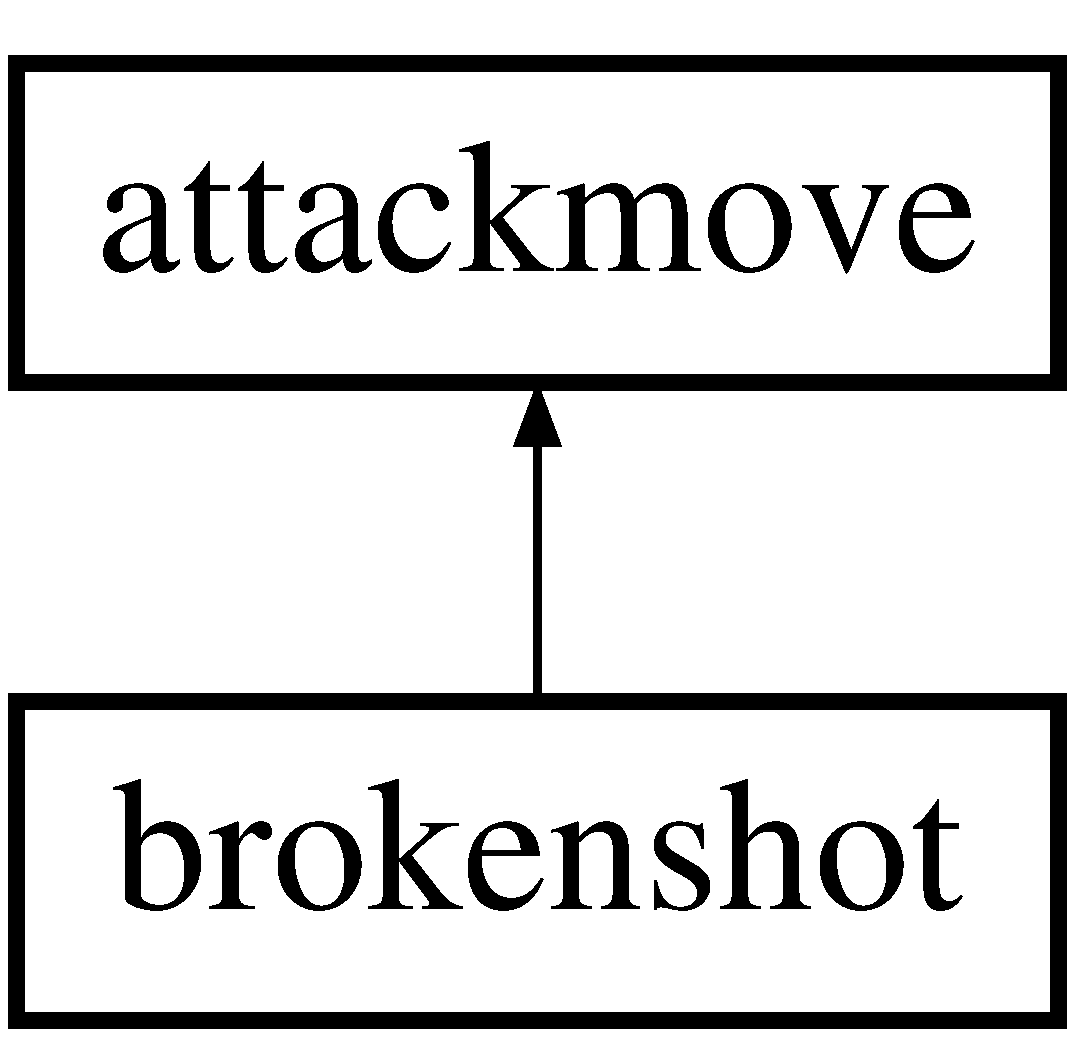
\includegraphics[height=2.000000cm]{classbrokenshot}
\end{center}
\end{figure}
\subsection*{Public Member Functions}
\begin{DoxyCompactItemize}
\item 
\hypertarget{classbrokenshot_aef0d22efead95c42a51a76293cfd91ae}{{\bfseries brokenshot} (int dam)}\label{classbrokenshot_aef0d22efead95c42a51a76293cfd91ae}

\item 
virtual Q\-String \hyperlink{classbrokenshot_a4834069bb57b3bb17a4816888cc83e43}{get\-String} ()
\begin{DoxyCompactList}\small\item\em \hyperlink{classattackmove_ada49eedf4b893372c576edd48fe73161}{attackmove\-::get\-String} \end{DoxyCompactList}\item 
virtual Q\-Image \hyperlink{classbrokenshot_ab5a534dcbeb99a57362e22bd11598a27}{get\-Image} ()
\begin{DoxyCompactList}\small\item\em \hyperlink{classattackmove_aca59a2343b7a6c195d300dda5c8d952d}{attackmove\-::get\-Image} \end{DoxyCompactList}\item 
virtual void \hyperlink{classbrokenshot_a1d9aaa51c4a27d8bb68a8f0678430d3a}{get\-Hover} (int hpanel, \hyperlink{class_enemy}{Enemy} $\ast$Enemies\mbox{[}3\mbox{]}, \hyperlink{classanim_items}{anim\-Items} $\ast$anim)
\begin{DoxyCompactList}\small\item\em \hyperlink{classattackmove_a0ff82349551bd72f4d57b3367bb318fa}{attackmove\-::get\-Hover} \end{DoxyCompactList}\item 
\hypertarget{classbrokenshot_a22b66a06882a1e1761fd796c7548cf50}{virtual void {\bfseries do\-Attack} (int hpanel, \hyperlink{class_enemy}{Enemy} $\ast$Enemies\mbox{[}$\,$\mbox{]}, \hyperlink{classanim_items}{anim\-Items} $\ast$anim)}\label{classbrokenshot_a22b66a06882a1e1761fd796c7548cf50}

\end{DoxyCompactItemize}
\subsection*{Additional Inherited Members}


\subsection{Member Function Documentation}
\hypertarget{classbrokenshot_a1d9aaa51c4a27d8bb68a8f0678430d3a}{\index{brokenshot@{brokenshot}!get\-Hover@{get\-Hover}}
\index{get\-Hover@{get\-Hover}!brokenshot@{brokenshot}}
\subsubsection[{get\-Hover}]{\setlength{\rightskip}{0pt plus 5cm}void brokenshot\-::get\-Hover (
\begin{DoxyParamCaption}
\item[{int}]{hpanel, }
\item[{{\bf Enemy} $\ast$}]{Enemies\mbox{[}3\mbox{]}, }
\item[{{\bf anim\-Items} $\ast$}]{anim}
\end{DoxyParamCaption}
)\hspace{0.3cm}{\ttfamily [virtual]}}}\label{classbrokenshot_a1d9aaa51c4a27d8bb68a8f0678430d3a}


\hyperlink{classattackmove_a0ff82349551bd72f4d57b3367bb318fa}{attackmove\-::get\-Hover} 


\begin{DoxyParams}{Parameters}
{\em hpanel} & \\
\hline
{\em Enemies} & \\
\hline
{\em anim} & \\
\hline
\end{DoxyParams}


Reimplemented from \hyperlink{classattackmove_a0ff82349551bd72f4d57b3367bb318fa}{attackmove}.

\hypertarget{classbrokenshot_ab5a534dcbeb99a57362e22bd11598a27}{\index{brokenshot@{brokenshot}!get\-Image@{get\-Image}}
\index{get\-Image@{get\-Image}!brokenshot@{brokenshot}}
\subsubsection[{get\-Image}]{\setlength{\rightskip}{0pt plus 5cm}Q\-Image brokenshot\-::get\-Image (
\begin{DoxyParamCaption}
{}
\end{DoxyParamCaption}
)\hspace{0.3cm}{\ttfamily [virtual]}}}\label{classbrokenshot_ab5a534dcbeb99a57362e22bd11598a27}


\hyperlink{classattackmove_aca59a2343b7a6c195d300dda5c8d952d}{attackmove\-::get\-Image} 

\begin{DoxyReturn}{Returns}

\end{DoxyReturn}


Reimplemented from \hyperlink{classattackmove_aca59a2343b7a6c195d300dda5c8d952d}{attackmove}.

\hypertarget{classbrokenshot_a4834069bb57b3bb17a4816888cc83e43}{\index{brokenshot@{brokenshot}!get\-String@{get\-String}}
\index{get\-String@{get\-String}!brokenshot@{brokenshot}}
\subsubsection[{get\-String}]{\setlength{\rightskip}{0pt plus 5cm}Q\-String brokenshot\-::get\-String (
\begin{DoxyParamCaption}
{}
\end{DoxyParamCaption}
)\hspace{0.3cm}{\ttfamily [virtual]}}}\label{classbrokenshot_a4834069bb57b3bb17a4816888cc83e43}


\hyperlink{classattackmove_ada49eedf4b893372c576edd48fe73161}{attackmove\-::get\-String} 

\begin{DoxyReturn}{Returns}
string of name, implemented in all inheritences includes damage 
\end{DoxyReturn}


Reimplemented from \hyperlink{classattackmove_ada49eedf4b893372c576edd48fe73161}{attackmove}.



The documentation for this class was generated from the following files\-:\begin{DoxyCompactItemize}
\item 
brokenshot.\-h\item 
brokenshot.\-cpp\end{DoxyCompactItemize}

\hypertarget{class_cannon}{\section{Cannon Class Reference}
\label{class_cannon}\index{Cannon@{Cannon}}
}
Inheritance diagram for Cannon\-:\begin{figure}[H]
\begin{center}
\leavevmode
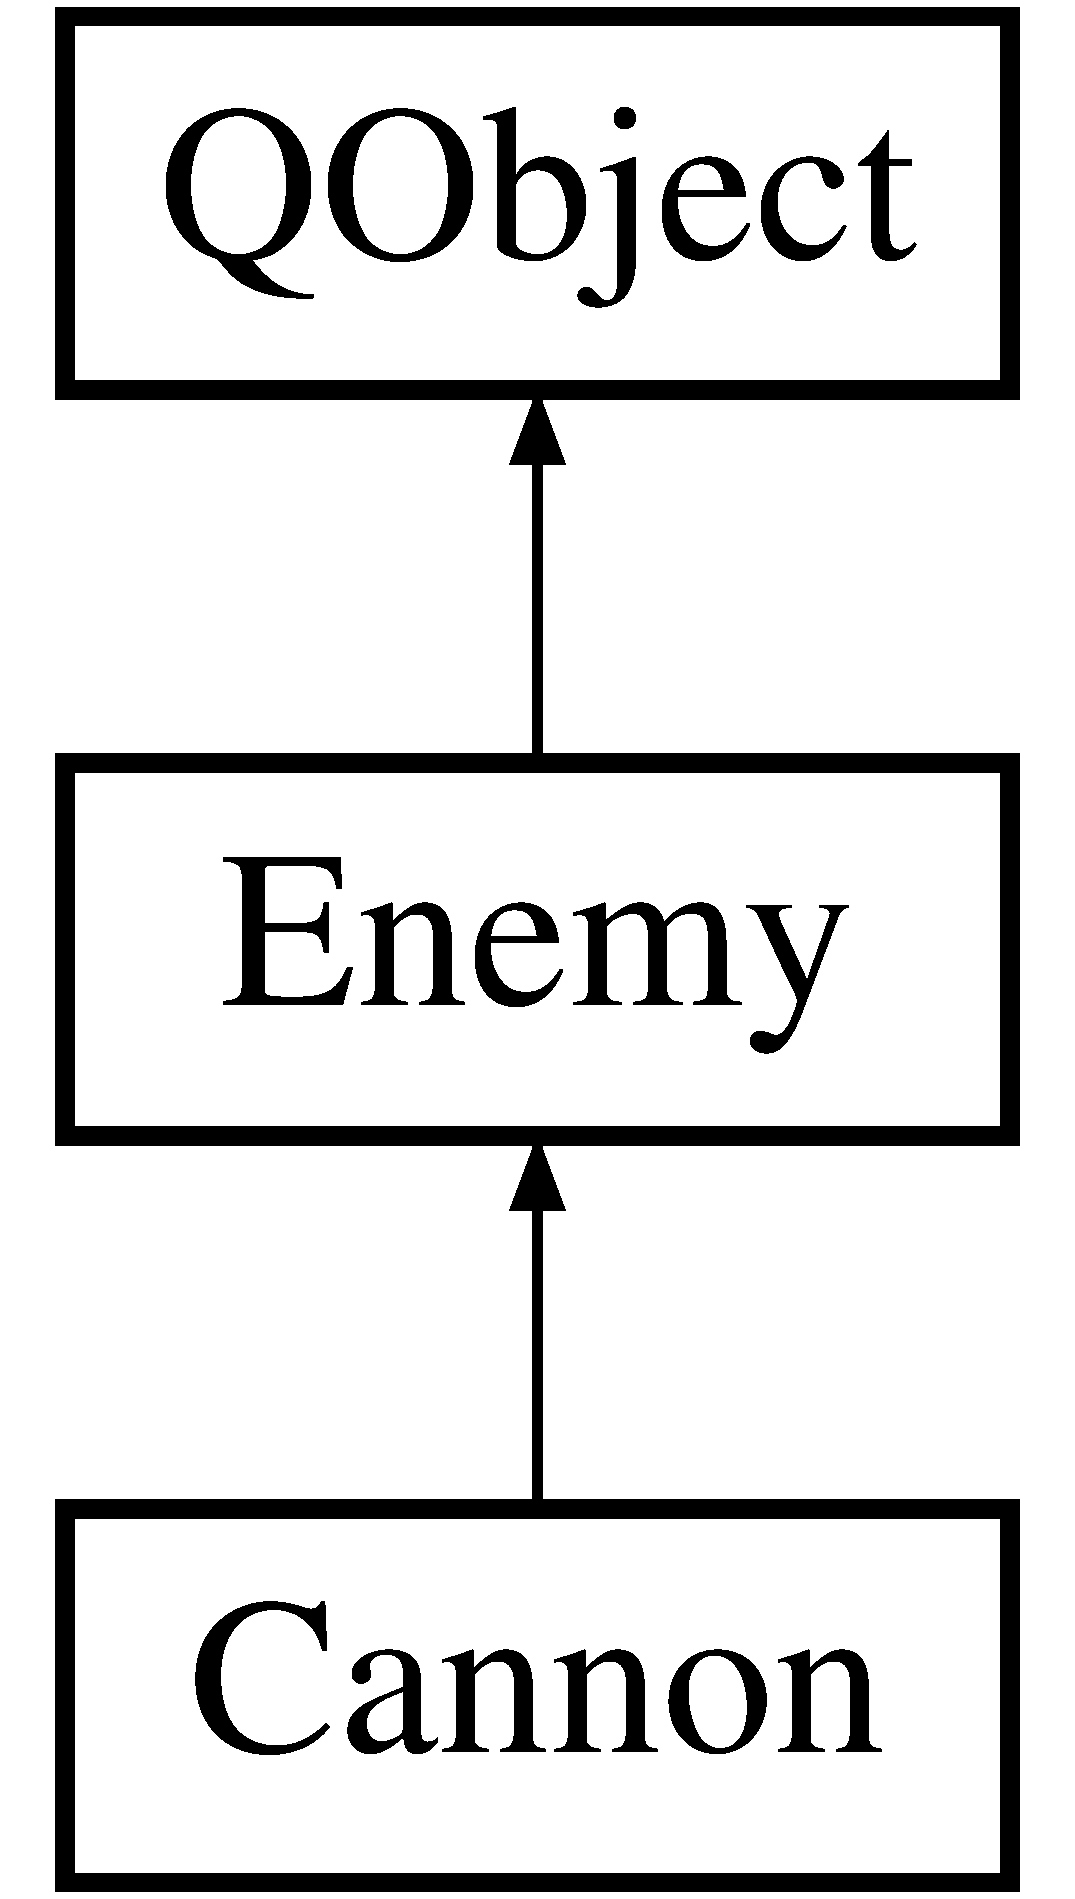
\includegraphics[height=3.000000cm]{class_cannon}
\end{center}
\end{figure}
\subsection*{Public Member Functions}
\begin{DoxyCompactItemize}
\item 
\hypertarget{class_cannon_a167a36b440912282d8c0b44c93afd20d}{{\bfseries Cannon} (int clev, int cx, int cy)}\label{class_cannon_a167a36b440912282d8c0b44c93afd20d}

\item 
virtual void \hyperlink{class_cannon_a0ac51832424376a120add27a8b8f2759}{do\-Turn} (\hyperlink{class_character}{Character} $\ast$Hero)
\begin{DoxyCompactList}\small\item\em \hyperlink{class_enemy_a56e4b9b07e8cd2a4e5ecfa8ff5b9265a}{Enemy\-::do\-Turn} based on hero's panel, does it's move. \end{DoxyCompactList}\item 
\hypertarget{class_cannon_a38f8c0c7f785ee10df1d83c8274ce546}{int {\bfseries get\-Ctr} ()}\label{class_cannon_a38f8c0c7f785ee10df1d83c8274ce546}

\item 
\hypertarget{class_cannon_acd2aee39d3e6b40681c69d44626ce6dd}{virtual Q\-Image {\bfseries get\-Pic} ()}\label{class_cannon_acd2aee39d3e6b40681c69d44626ce6dd}

\item 
virtual void \hyperlink{class_cannon_ab3893b885bdc31461a6cacb072b223a3}{draw\-Self} (Q\-Painter $\ast$g, int gx, int gy)
\begin{DoxyCompactList}\small\item\em \hyperlink{class_enemy_a3251244e8e7ac657687d6be5a8da71bb}{Enemy\-::draw\-Self} draws itself using painter, includes title and hp. \end{DoxyCompactList}\end{DoxyCompactItemize}
\subsection*{Additional Inherited Members}


\subsection{Member Function Documentation}
\hypertarget{class_cannon_a0ac51832424376a120add27a8b8f2759}{\index{Cannon@{Cannon}!do\-Turn@{do\-Turn}}
\index{do\-Turn@{do\-Turn}!Cannon@{Cannon}}
\subsubsection[{do\-Turn}]{\setlength{\rightskip}{0pt plus 5cm}void Cannon\-::do\-Turn (
\begin{DoxyParamCaption}
\item[{{\bf Character} $\ast$}]{Hero}
\end{DoxyParamCaption}
)\hspace{0.3cm}{\ttfamily [virtual]}}}\label{class_cannon_a0ac51832424376a120add27a8b8f2759}


\hyperlink{class_enemy_a56e4b9b07e8cd2a4e5ecfa8ff5b9265a}{Enemy\-::do\-Turn} based on hero's panel, does it's move. 


\begin{DoxyParams}{Parameters}
{\em Hero} & \\
\hline
\end{DoxyParams}


Reimplemented from \hyperlink{class_enemy_a56e4b9b07e8cd2a4e5ecfa8ff5b9265a}{Enemy}.

\hypertarget{class_cannon_ab3893b885bdc31461a6cacb072b223a3}{\index{Cannon@{Cannon}!draw\-Self@{draw\-Self}}
\index{draw\-Self@{draw\-Self}!Cannon@{Cannon}}
\subsubsection[{draw\-Self}]{\setlength{\rightskip}{0pt plus 5cm}void Cannon\-::draw\-Self (
\begin{DoxyParamCaption}
\item[{Q\-Painter $\ast$}]{g, }
\item[{int}]{gx, }
\item[{int}]{gy}
\end{DoxyParamCaption}
)\hspace{0.3cm}{\ttfamily [virtual]}}}\label{class_cannon_ab3893b885bdc31461a6cacb072b223a3}


\hyperlink{class_enemy_a3251244e8e7ac657687d6be5a8da71bb}{Enemy\-::draw\-Self} draws itself using painter, includes title and hp. 


\begin{DoxyParams}{Parameters}
{\em g} & \\
\hline
{\em gx} & \\
\hline
{\em gy} & \\
\hline
\end{DoxyParams}


Reimplemented from \hyperlink{class_enemy_a3251244e8e7ac657687d6be5a8da71bb}{Enemy}.



The documentation for this class was generated from the following files\-:\begin{DoxyCompactItemize}
\item 
cannon.\-h\item 
cannon.\-cpp\end{DoxyCompactItemize}

\hypertarget{class_character}{\section{Character Class Reference}
\label{class_character}\index{Character@{Character}}
}
\subsection*{Public Member Functions}
\begin{DoxyCompactItemize}
\item 
\hyperlink{class_character_a663231826f9b61c5802228f9b7b743ad}{Character} (int start\-H\-P, int sexp, int cdam, int cpanel)
\begin{DoxyCompactList}\small\item\em \hyperlink{class_character_a663231826f9b61c5802228f9b7b743ad}{Character\-::\-Character} main hero character used in battle. \end{DoxyCompactList}\item 
bool \hyperlink{class_character_af92b5cb1ab23f30e9aa3371e10e331fe}{get\-Damaged} (int damage)
\begin{DoxyCompactList}\small\item\em \hyperlink{class_character_af92b5cb1ab23f30e9aa3371e10e331fe}{Character\-::get\-Damaged}. \end{DoxyCompactList}\item 
void \hyperlink{class_character_a9e80c446cdcb4651dc321adc80125999}{get\-Restored} (int recovery)
\begin{DoxyCompactList}\small\item\em \hyperlink{class_character_a9e80c446cdcb4651dc321adc80125999}{Character\-::get\-Restored} if already at max, stays at max. \end{DoxyCompactList}\item 
\hypertarget{class_character_a6f222adddaed0b313094d33700251c6b}{int {\bfseries get\-H\-P} ()}\label{class_character_a6f222adddaed0b313094d33700251c6b}

\item 
\hypertarget{class_character_a0cc4b7dbbaad0f639db856ddfca2e268}{int {\bfseries getexp} ()}\label{class_character_a0cc4b7dbbaad0f639db856ddfca2e268}

\item 
\hypertarget{class_character_a67f56cdab1f01f561073dfcdcf228fda}{int {\bfseries getmax\-H\-P} ()}\label{class_character_a67f56cdab1f01f561073dfcdcf228fda}

\item 
\hypertarget{class_character_a5ee4e596c276d23c486f564c25afe11c}{void {\bfseries set\-H\-P} (int nhp)}\label{class_character_a5ee4e596c276d23c486f564c25afe11c}

\item 
\hypertarget{class_character_afdc04a22ede639e575e6dfc10b15bbcd}{void {\bfseries setexp} (int nexp)}\label{class_character_afdc04a22ede639e575e6dfc10b15bbcd}

\item 
\hypertarget{class_character_ad758a1dde55f9487dccca36ded607a48}{void {\bfseries setmax\-H\-P} (int nmaxhp)}\label{class_character_ad758a1dde55f9487dccca36ded607a48}

\item 
\hypertarget{class_character_ae2ae019ff6d7b8150113fd8add961f39}{void {\bfseries set\-Can\-Move} (bool cmove)}\label{class_character_ae2ae019ff6d7b8150113fd8add961f39}

\item 
\hypertarget{class_character_a5d2616851987d4f844b2c440636f6b7f}{bool {\bfseries get\-Can\-Move} ()}\label{class_character_a5d2616851987d4f844b2c440636f6b7f}

\item 
\hypertarget{class_character_a104dd581ebc631f1b9448abf47d6cb46}{int {\bfseries get\-Panel} ()}\label{class_character_a104dd581ebc631f1b9448abf47d6cb46}

\item 
\hypertarget{class_character_aa3c91db87d4e4ccee3a5bdc9546084de}{void {\bfseries set\-Panel} (int cpanel)}\label{class_character_aa3c91db87d4e4ccee3a5bdc9546084de}

\item 
\hypertarget{class_character_a8173beca9b6a1aee4213156f44f73708}{void {\bfseries set\-Turn} (bool cturn)}\label{class_character_a8173beca9b6a1aee4213156f44f73708}

\item 
\hypertarget{class_character_afad175e9eb494ea86fb3f3f03becbf86}{bool {\bfseries is\-Turn} ()}\label{class_character_afad175e9eb494ea86fb3f3f03becbf86}

\item 
\hypertarget{class_character_ae5614f09a48cab021451e1d174c49f40}{void {\bfseries set\-Dam} (int cdam)}\label{class_character_ae5614f09a48cab021451e1d174c49f40}

\item 
\hypertarget{class_character_a22e0b2d268c078a0a2055bc547c13779}{int {\bfseries get\-Dam} ()}\label{class_character_a22e0b2d268c078a0a2055bc547c13779}

\item 
int \hyperlink{class_character_af20f9fcc4dc0439c3d33463d52f62baa}{get\-Gold} ()
\begin{DoxyCompactList}\small\item\em \hyperlink{class_character_af20f9fcc4dc0439c3d33463d52f62baa}{Character\-::get\-Gold}. \end{DoxyCompactList}\item 
void \hyperlink{class_character_a022b611a56f1c4a87972de352b9c58ed}{inc\-Gold} (int amt)
\begin{DoxyCompactList}\small\item\em \hyperlink{class_character_a022b611a56f1c4a87972de352b9c58ed}{Character\-::inc\-Gold}. \end{DoxyCompactList}\end{DoxyCompactItemize}
\subsection*{Public Attributes}
\begin{DoxyCompactItemize}
\item 
\hypertarget{class_character_ab8dd866071dba429a35555e0c372e162}{int {\bfseries gold}}\label{class_character_ab8dd866071dba429a35555e0c372e162}

\end{DoxyCompactItemize}


\subsection{Constructor \& Destructor Documentation}
\hypertarget{class_character_a663231826f9b61c5802228f9b7b743ad}{\index{Character@{Character}!Character@{Character}}
\index{Character@{Character}!Character@{Character}}
\subsubsection[{Character}]{\setlength{\rightskip}{0pt plus 5cm}Character\-::\-Character (
\begin{DoxyParamCaption}
\item[{int}]{start\-H\-P, }
\item[{int}]{sexp, }
\item[{int}]{cdam, }
\item[{int}]{cpanel}
\end{DoxyParamCaption}
)}}\label{class_character_a663231826f9b61c5802228f9b7b743ad}


\hyperlink{class_character_a663231826f9b61c5802228f9b7b743ad}{Character\-::\-Character} main hero character used in battle. 


\begin{DoxyParams}{Parameters}
{\em start\-H\-P} & \\
\hline
{\em sexp} & \\
\hline
{\em cdam} & \\
\hline
{\em cpanel} & \\
\hline
\end{DoxyParams}


\subsection{Member Function Documentation}
\hypertarget{class_character_af92b5cb1ab23f30e9aa3371e10e331fe}{\index{Character@{Character}!get\-Damaged@{get\-Damaged}}
\index{get\-Damaged@{get\-Damaged}!Character@{Character}}
\subsubsection[{get\-Damaged}]{\setlength{\rightskip}{0pt plus 5cm}bool Character\-::get\-Damaged (
\begin{DoxyParamCaption}
\item[{int}]{damage}
\end{DoxyParamCaption}
)}}\label{class_character_af92b5cb1ab23f30e9aa3371e10e331fe}


\hyperlink{class_character_af92b5cb1ab23f30e9aa3371e10e331fe}{Character\-::get\-Damaged}. 


\begin{DoxyParams}{Parameters}
{\em damage} & \\
\hline
\end{DoxyParams}
\begin{DoxyReturn}{Returns}

\end{DoxyReturn}
\hypertarget{class_character_af20f9fcc4dc0439c3d33463d52f62baa}{\index{Character@{Character}!get\-Gold@{get\-Gold}}
\index{get\-Gold@{get\-Gold}!Character@{Character}}
\subsubsection[{get\-Gold}]{\setlength{\rightskip}{0pt plus 5cm}int Character\-::get\-Gold (
\begin{DoxyParamCaption}
{}
\end{DoxyParamCaption}
)}}\label{class_character_af20f9fcc4dc0439c3d33463d52f62baa}


\hyperlink{class_character_af20f9fcc4dc0439c3d33463d52f62baa}{Character\-::get\-Gold}. 

\begin{DoxyReturn}{Returns}
gold character has 
\end{DoxyReturn}
\hypertarget{class_character_a9e80c446cdcb4651dc321adc80125999}{\index{Character@{Character}!get\-Restored@{get\-Restored}}
\index{get\-Restored@{get\-Restored}!Character@{Character}}
\subsubsection[{get\-Restored}]{\setlength{\rightskip}{0pt plus 5cm}void Character\-::get\-Restored (
\begin{DoxyParamCaption}
\item[{int}]{recovery}
\end{DoxyParamCaption}
)}}\label{class_character_a9e80c446cdcb4651dc321adc80125999}


\hyperlink{class_character_a9e80c446cdcb4651dc321adc80125999}{Character\-::get\-Restored} if already at max, stays at max. 


\begin{DoxyParams}{Parameters}
{\em recovery} & \\
\hline
\end{DoxyParams}
\hypertarget{class_character_a022b611a56f1c4a87972de352b9c58ed}{\index{Character@{Character}!inc\-Gold@{inc\-Gold}}
\index{inc\-Gold@{inc\-Gold}!Character@{Character}}
\subsubsection[{inc\-Gold}]{\setlength{\rightskip}{0pt plus 5cm}void Character\-::inc\-Gold (
\begin{DoxyParamCaption}
\item[{int}]{amt}
\end{DoxyParamCaption}
)}}\label{class_character_a022b611a56f1c4a87972de352b9c58ed}


\hyperlink{class_character_a022b611a56f1c4a87972de352b9c58ed}{Character\-::inc\-Gold}. 


\begin{DoxyParams}{Parameters}
{\em amt} & of gold to increase \\
\hline
\end{DoxyParams}


The documentation for this class was generated from the following files\-:\begin{DoxyCompactItemize}
\item 
character.\-h\item 
character.\-cpp\end{DoxyCompactItemize}

\hypertarget{class_circle_widget}{\section{Circle\-Widget Class Reference}
\label{class_circle_widget}\index{Circle\-Widget@{Circle\-Widget}}
}


\mbox{[}0\mbox{]}  




{\ttfamily \#include $<$circlewidget.\-h$>$}

Inheritance diagram for Circle\-Widget\-:\begin{figure}[H]
\begin{center}
\leavevmode
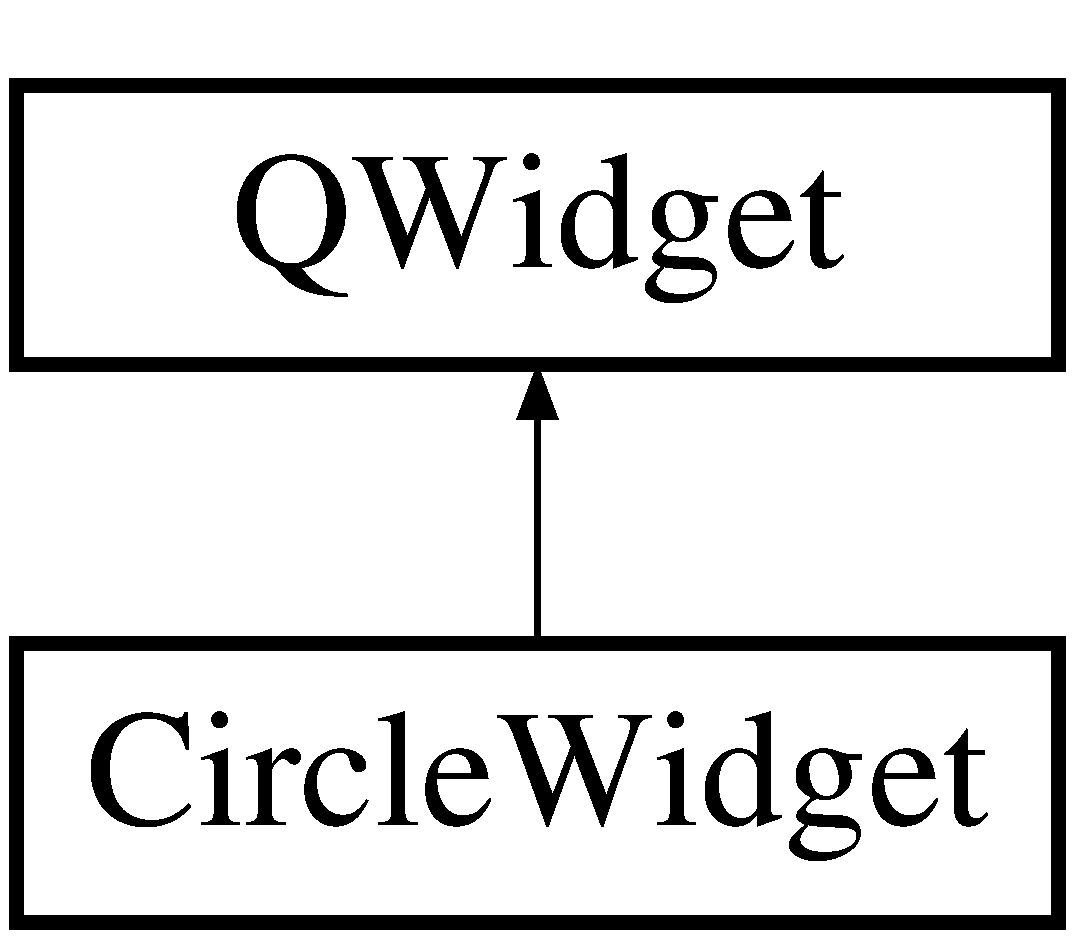
\includegraphics[height=2.000000cm]{class_circle_widget}
\end{center}
\end{figure}
\subsection*{Public Types}
\begin{DoxyCompactItemize}
\item 
enum {\bfseries Color\-Kind} \{ {\bfseries R\-E\-D}, 
{\bfseries G\-R\-E\-E\-N}, 
{\bfseries B\-L\-U\-E}
 \}
\end{DoxyCompactItemize}
\subsection*{Public Slots}
\begin{DoxyCompactItemize}
\item 
void \hyperlink{class_circle_widget_ae98951095744e9f6ceb446093270fe03}{next\-Animation\-Frame} ()
\begin{DoxyCompactList}\small\item\em \mbox{[}4\mbox{]} \end{DoxyCompactList}\item 
\hypertarget{class_circle_widget_a070cd25f6215b86de995b3b9a4970a06}{void \hyperlink{class_circle_widget_a070cd25f6215b86de995b3b9a4970a06}{slot\-\_\-timeout} ()}\label{class_circle_widget_a070cd25f6215b86de995b3b9a4970a06}

\begin{DoxyCompactList}\small\item\em \mbox{[}5\mbox{]} \end{DoxyCompactList}\end{DoxyCompactItemize}
\subsection*{Public Member Functions}
\begin{DoxyCompactItemize}
\item 
\hypertarget{class_circle_widget_a457a279772f9655749433cc9d6d375d7}{\hyperlink{class_circle_widget_a457a279772f9655749433cc9d6d375d7}{Circle\-Widget} (Q\-Widget $\ast$parent=0)}\label{class_circle_widget_a457a279772f9655749433cc9d6d375d7}

\begin{DoxyCompactList}\small\item\em \mbox{[}0\mbox{]} \end{DoxyCompactList}\item 
void \hyperlink{class_circle_widget_ac69fe4d274d4b3c2df87f3acfa61e583}{set\-Float\-Based} (bool float\-Based)
\begin{DoxyCompactList}\small\item\em \mbox{[}0\mbox{]} \end{DoxyCompactList}\item 
void \hyperlink{class_circle_widget_ad3fc2e4312f4f832fce806167e963c2c}{set\-Antialiased} (bool antialiased)
\begin{DoxyCompactList}\small\item\em \mbox{[}1\mbox{]} \end{DoxyCompactList}\item 
\hypertarget{class_circle_widget_a8d634df7bdacffd407cdb0ca47e8ab67}{void \hyperlink{class_circle_widget_a8d634df7bdacffd407cdb0ca47e8ab67}{set\-Color\-Kind} (Color\-Kind c)}\label{class_circle_widget_a8d634df7bdacffd407cdb0ca47e8ab67}

\begin{DoxyCompactList}\small\item\em \mbox{[}2\mbox{]} \end{DoxyCompactList}\item 
\hypertarget{class_circle_widget_adef54ffc91f67df88c60ffe380ed3691}{Q\-Size \hyperlink{class_circle_widget_adef54ffc91f67df88c60ffe380ed3691}{minimum\-Size\-Hint} () const }\label{class_circle_widget_adef54ffc91f67df88c60ffe380ed3691}

\begin{DoxyCompactList}\small\item\em \mbox{[}3\mbox{]} \end{DoxyCompactList}\item 
Q\-Size \hyperlink{class_circle_widget_ac4305a08d1734e5c79cd1cb86ba3033e}{size\-Hint} () const 
\begin{DoxyCompactList}\small\item\em \mbox{[}3\mbox{]} \end{DoxyCompactList}\end{DoxyCompactItemize}
\subsection*{Protected Member Functions}
\begin{DoxyCompactItemize}
\item 
void \hyperlink{class_circle_widget_af5b0bee26a5a3c6709325bac6353f17f}{paint\-Event} (Q\-Paint\-Event $\ast$event)
\begin{DoxyCompactList}\small\item\em \mbox{[}6\mbox{]} \end{DoxyCompactList}\end{DoxyCompactItemize}


\subsection{Detailed Description}
\mbox{[}0\mbox{]} 

\subsection{Member Function Documentation}
\hypertarget{class_circle_widget_ae98951095744e9f6ceb446093270fe03}{\index{Circle\-Widget@{Circle\-Widget}!next\-Animation\-Frame@{next\-Animation\-Frame}}
\index{next\-Animation\-Frame@{next\-Animation\-Frame}!CircleWidget@{Circle\-Widget}}
\subsubsection[{next\-Animation\-Frame}]{\setlength{\rightskip}{0pt plus 5cm}void Circle\-Widget\-::next\-Animation\-Frame (
\begin{DoxyParamCaption}
{}
\end{DoxyParamCaption}
)\hspace{0.3cm}{\ttfamily [slot]}}}\label{class_circle_widget_ae98951095744e9f6ceb446093270fe03}


\mbox{[}4\mbox{]} 

\mbox{[}5\mbox{]} \hypertarget{class_circle_widget_af5b0bee26a5a3c6709325bac6353f17f}{\index{Circle\-Widget@{Circle\-Widget}!paint\-Event@{paint\-Event}}
\index{paint\-Event@{paint\-Event}!CircleWidget@{Circle\-Widget}}
\subsubsection[{paint\-Event}]{\setlength{\rightskip}{0pt plus 5cm}void Circle\-Widget\-::paint\-Event (
\begin{DoxyParamCaption}
\item[{Q\-Paint\-Event $\ast$}]{event}
\end{DoxyParamCaption}
)\hspace{0.3cm}{\ttfamily [protected]}}}\label{class_circle_widget_af5b0bee26a5a3c6709325bac6353f17f}


\mbox{[}6\mbox{]} 

\mbox{[}6\mbox{]}

\mbox{[}7\mbox{]}

\mbox{[}7\mbox{]} //! \mbox{[}8\mbox{]} \hypertarget{class_circle_widget_ad3fc2e4312f4f832fce806167e963c2c}{\index{Circle\-Widget@{Circle\-Widget}!set\-Antialiased@{set\-Antialiased}}
\index{set\-Antialiased@{set\-Antialiased}!CircleWidget@{Circle\-Widget}}
\subsubsection[{set\-Antialiased}]{\setlength{\rightskip}{0pt plus 5cm}void Circle\-Widget\-::set\-Antialiased (
\begin{DoxyParamCaption}
\item[{bool}]{antialiased}
\end{DoxyParamCaption}
)}}\label{class_circle_widget_ad3fc2e4312f4f832fce806167e963c2c}


\mbox{[}1\mbox{]} 

\mbox{[}2\mbox{]} \hypertarget{class_circle_widget_ac69fe4d274d4b3c2df87f3acfa61e583}{\index{Circle\-Widget@{Circle\-Widget}!set\-Float\-Based@{set\-Float\-Based}}
\index{set\-Float\-Based@{set\-Float\-Based}!CircleWidget@{Circle\-Widget}}
\subsubsection[{set\-Float\-Based}]{\setlength{\rightskip}{0pt plus 5cm}void Circle\-Widget\-::set\-Float\-Based (
\begin{DoxyParamCaption}
\item[{bool}]{float\-Based}
\end{DoxyParamCaption}
)}}\label{class_circle_widget_ac69fe4d274d4b3c2df87f3acfa61e583}


\mbox{[}0\mbox{]} 

\mbox{[}1\mbox{]} \hypertarget{class_circle_widget_ac4305a08d1734e5c79cd1cb86ba3033e}{\index{Circle\-Widget@{Circle\-Widget}!size\-Hint@{size\-Hint}}
\index{size\-Hint@{size\-Hint}!CircleWidget@{Circle\-Widget}}
\subsubsection[{size\-Hint}]{\setlength{\rightskip}{0pt plus 5cm}Q\-Size Circle\-Widget\-::size\-Hint (
\begin{DoxyParamCaption}
{}
\end{DoxyParamCaption}
) const}}\label{class_circle_widget_ac4305a08d1734e5c79cd1cb86ba3033e}


\mbox{[}3\mbox{]} 

\mbox{[}4\mbox{]} 

The documentation for this class was generated from the following files\-:\begin{DoxyCompactItemize}
\item 
circlewidget.\-h\item 
circlewidget.\-cpp\end{DoxyCompactItemize}

\hypertarget{class_enemy}{\section{Enemy Class Reference}
\label{class_enemy}\index{Enemy@{Enemy}}
}
Inheritance diagram for Enemy\-:\begin{figure}[H]
\begin{center}
\leavevmode
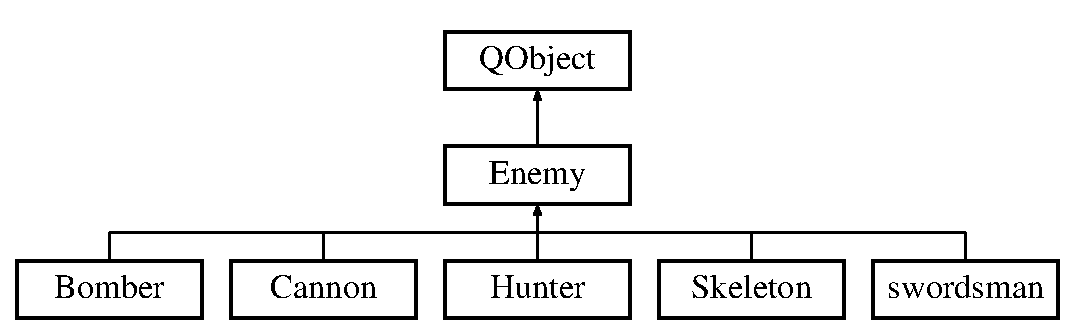
\includegraphics[height=3.000000cm]{class_enemy}
\end{center}
\end{figure}
\subsection*{Public Member Functions}
\begin{DoxyCompactItemize}
\item 
\hyperlink{class_enemy_a0638b6e9f11a72831051438dbf803d91}{Enemy} (int clev, int cx, int cy)
\begin{DoxyCompactList}\small\item\em \hyperlink{class_enemy_a0638b6e9f11a72831051438dbf803d91}{Enemy\-::\-Enemy}. \end{DoxyCompactList}\item 
\hypertarget{class_enemy_a0ebc35bd4cd41e81df912b6286426c46}{void {\bfseries set\-X} (int cx)}\label{class_enemy_a0ebc35bd4cd41e81df912b6286426c46}

\item 
\hypertarget{class_enemy_a1fab961fbc5b1fd1764515c1a00f424b}{void {\bfseries set\-Y} (int cy)}\label{class_enemy_a1fab961fbc5b1fd1764515c1a00f424b}

\item 
\hypertarget{class_enemy_aa07b45a0163d1c16326dc8706ec77414}{void {\bfseries set\-Turn} (bool cmove)}\label{class_enemy_aa07b45a0163d1c16326dc8706ec77414}

\item 
\hypertarget{class_enemy_a8742266192bffefd0746d5665e816463}{void {\bfseries set\-Move} (bool cmove)}\label{class_enemy_a8742266192bffefd0746d5665e816463}

\item 
\hypertarget{class_enemy_abdd71d2a54bf169ffb71801091704881}{int {\bfseries get\-X} ()}\label{class_enemy_abdd71d2a54bf169ffb71801091704881}

\item 
\hypertarget{class_enemy_a056667d7235d861cdc88ecfe2341ca90}{int {\bfseries get\-Y} ()}\label{class_enemy_a056667d7235d861cdc88ecfe2341ca90}

\item 
\hypertarget{class_enemy_a742cf2ff493fd15a4a11a13e20e60423}{bool {\bfseries get\-Move} ()}\label{class_enemy_a742cf2ff493fd15a4a11a13e20e60423}

\item 
\hypertarget{class_enemy_ad25491cf4bd75217a4d97318f0ec0677}{bool {\bfseries get\-Turn} ()}\label{class_enemy_ad25491cf4bd75217a4d97318f0ec0677}

\item 
\hypertarget{class_enemy_ab1c5ecbd2567b509a5d4492764a28f5d}{int {\bfseries get\-H\-P} ()}\label{class_enemy_ab1c5ecbd2567b509a5d4492764a28f5d}

\item 
\hypertarget{class_enemy_a32c6b8b1784ff8301c1cb20d969bb6bb}{int {\bfseries getmax\-H\-P} ()}\label{class_enemy_a32c6b8b1784ff8301c1cb20d969bb6bb}

\item 
\hypertarget{class_enemy_a4c6c4bfd244315ba6cfd338428f33d48}{bool {\bfseries get\-Alive} ()}\label{class_enemy_a4c6c4bfd244315ba6cfd338428f33d48}

\item 
\hypertarget{class_enemy_aa9ed76dea0526fba28e15e9667a9eb25}{void {\bfseries set\-Alive} (bool is\-Alive)}\label{class_enemy_aa9ed76dea0526fba28e15e9667a9eb25}

\item 
virtual void \hyperlink{class_enemy_a56e4b9b07e8cd2a4e5ecfa8ff5b9265a}{do\-Turn} (\hyperlink{class_character}{Character} $\ast$Hero)
\begin{DoxyCompactList}\small\item\em \hyperlink{class_enemy_a56e4b9b07e8cd2a4e5ecfa8ff5b9265a}{Enemy\-::do\-Turn} based on hero's panel, does it's move. \end{DoxyCompactList}\item 
\hypertarget{class_enemy_a577a10f1cd0eb2bdd7f600c63044b010}{bool {\bfseries get\-Damaged} (int damage)}\label{class_enemy_a577a10f1cd0eb2bdd7f600c63044b010}

\item 
\hypertarget{class_enemy_a17b20f01b5af2ca88c844fb0f072f4fc}{void {\bfseries get\-Restored} (int recovery)}\label{class_enemy_a17b20f01b5af2ca88c844fb0f072f4fc}

\item 
\hypertarget{class_enemy_a7eb85dffc1f22c21eb6ff805192f3818}{virtual Q\-Image {\bfseries get\-Pic} ()}\label{class_enemy_a7eb85dffc1f22c21eb6ff805192f3818}

\item 
virtual void \hyperlink{class_enemy_a3251244e8e7ac657687d6be5a8da71bb}{draw\-Self} (Q\-Painter $\ast$g, int gx, int gy)
\begin{DoxyCompactList}\small\item\em \hyperlink{class_enemy_a3251244e8e7ac657687d6be5a8da71bb}{Enemy\-::draw\-Self} draws itself using painter, includes title and hp. \end{DoxyCompactList}\end{DoxyCompactItemize}
\subsection*{Protected Attributes}
\begin{DoxyCompactItemize}
\item 
\hypertarget{class_enemy_ab685146410b2972ccab930a522fd9252}{int {\bfseries xpos}}\label{class_enemy_ab685146410b2972ccab930a522fd9252}

\item 
\hypertarget{class_enemy_a7cb1bc241abdacc846ae2313f2a54bbc}{int {\bfseries ypos}}\label{class_enemy_a7cb1bc241abdacc846ae2313f2a54bbc}

\item 
\hypertarget{class_enemy_a2891f607bd7c05774ab7efaf155c1842}{int {\bfseries current\-H\-P}}\label{class_enemy_a2891f607bd7c05774ab7efaf155c1842}

\item 
\hypertarget{class_enemy_a990ecf4cbfdae850b51e6fb2b367ad8e}{int {\bfseries max\-H\-P}}\label{class_enemy_a990ecf4cbfdae850b51e6fb2b367ad8e}

\item 
\hypertarget{class_enemy_a09d68a627f0f664d0dd3ac8063dd5cb3}{int {\bfseries in\-Turn}}\label{class_enemy_a09d68a627f0f664d0dd3ac8063dd5cb3}

\item 
\hypertarget{class_enemy_a5bbd6ff8c998dc4a67badee154c9e453}{int {\bfseries canmove}}\label{class_enemy_a5bbd6ff8c998dc4a67badee154c9e453}

\item 
\hypertarget{class_enemy_a02481d9c8d5b64d4d83556e047fcda7b}{bool {\bfseries Alive}}\label{class_enemy_a02481d9c8d5b64d4d83556e047fcda7b}

\item 
\hypertarget{class_enemy_a4754b00e9ff05f83a293f74324016c17}{int {\bfseries level}}\label{class_enemy_a4754b00e9ff05f83a293f74324016c17}

\item 
\hypertarget{class_enemy_a4969f2e5372ae6840aba5cd0b8059a0a}{int {\bfseries damage}}\label{class_enemy_a4969f2e5372ae6840aba5cd0b8059a0a}

\end{DoxyCompactItemize}


\subsection{Constructor \& Destructor Documentation}
\hypertarget{class_enemy_a0638b6e9f11a72831051438dbf803d91}{\index{Enemy@{Enemy}!Enemy@{Enemy}}
\index{Enemy@{Enemy}!Enemy@{Enemy}}
\subsubsection[{Enemy}]{\setlength{\rightskip}{0pt plus 5cm}Enemy\-::\-Enemy (
\begin{DoxyParamCaption}
\item[{int}]{clev, }
\item[{int}]{cx, }
\item[{int}]{cy}
\end{DoxyParamCaption}
)}}\label{class_enemy_a0638b6e9f11a72831051438dbf803d91}


\hyperlink{class_enemy_a0638b6e9f11a72831051438dbf803d91}{Enemy\-::\-Enemy}. 


\begin{DoxyParams}{Parameters}
{\em clev} & level of character, different for each inheritance \\
\hline
{\em cx} & \\
\hline
{\em cy} & \\
\hline
\end{DoxyParams}


\subsection{Member Function Documentation}
\hypertarget{class_enemy_a56e4b9b07e8cd2a4e5ecfa8ff5b9265a}{\index{Enemy@{Enemy}!do\-Turn@{do\-Turn}}
\index{do\-Turn@{do\-Turn}!Enemy@{Enemy}}
\subsubsection[{do\-Turn}]{\setlength{\rightskip}{0pt plus 5cm}void Enemy\-::do\-Turn (
\begin{DoxyParamCaption}
\item[{{\bf Character} $\ast$}]{Hero}
\end{DoxyParamCaption}
)\hspace{0.3cm}{\ttfamily [virtual]}}}\label{class_enemy_a56e4b9b07e8cd2a4e5ecfa8ff5b9265a}


\hyperlink{class_enemy_a56e4b9b07e8cd2a4e5ecfa8ff5b9265a}{Enemy\-::do\-Turn} based on hero's panel, does it's move. 


\begin{DoxyParams}{Parameters}
{\em Hero} & \\
\hline
\end{DoxyParams}


Reimplemented in \hyperlink{class_bomber_ac0f488834e2abdab290699d6efa6e72e}{Bomber}, \hyperlink{class_cannon_a0ac51832424376a120add27a8b8f2759}{Cannon}, \hyperlink{class_hunter_a910f2c34961a3d7fb1caa91e65b5d743}{Hunter}, \hyperlink{class_skeleton_aeb5642a3aa8c49cb0cd1cc325f8f0baa}{Skeleton}, and \hyperlink{classswordsman_a99dec33c47dc5f3936229e5045b9c235}{swordsman}.

\hypertarget{class_enemy_a3251244e8e7ac657687d6be5a8da71bb}{\index{Enemy@{Enemy}!draw\-Self@{draw\-Self}}
\index{draw\-Self@{draw\-Self}!Enemy@{Enemy}}
\subsubsection[{draw\-Self}]{\setlength{\rightskip}{0pt plus 5cm}void Enemy\-::draw\-Self (
\begin{DoxyParamCaption}
\item[{Q\-Painter $\ast$}]{g, }
\item[{int}]{gx, }
\item[{int}]{gy}
\end{DoxyParamCaption}
)\hspace{0.3cm}{\ttfamily [virtual]}}}\label{class_enemy_a3251244e8e7ac657687d6be5a8da71bb}


\hyperlink{class_enemy_a3251244e8e7ac657687d6be5a8da71bb}{Enemy\-::draw\-Self} draws itself using painter, includes title and hp. 


\begin{DoxyParams}{Parameters}
{\em g} & \\
\hline
{\em gx} & \\
\hline
{\em gy} & \\
\hline
\end{DoxyParams}


Reimplemented in \hyperlink{class_bomber_aa75d9256efa7f2996a599deb3db83f90}{Bomber}, \hyperlink{class_cannon_ab3893b885bdc31461a6cacb072b223a3}{Cannon}, \hyperlink{class_hunter_a765f282edf2fd27998740d33ed81a423}{Hunter}, \hyperlink{class_skeleton_ae605f24f6e921ad3b36a53f391304722}{Skeleton}, and \hyperlink{classswordsman_ad897e7c34033347faa5e4022b27cc395}{swordsman}.



The documentation for this class was generated from the following files\-:\begin{DoxyCompactItemize}
\item 
enemy.\-h\item 
enemy.\-cpp\end{DoxyCompactItemize}

\hypertarget{class_graphics_view}{\section{Graphics\-View Class Reference}
\label{class_graphics_view}\index{Graphics\-View@{Graphics\-View}}
}
Inheritance diagram for Graphics\-View\-:\begin{figure}[H]
\begin{center}
\leavevmode
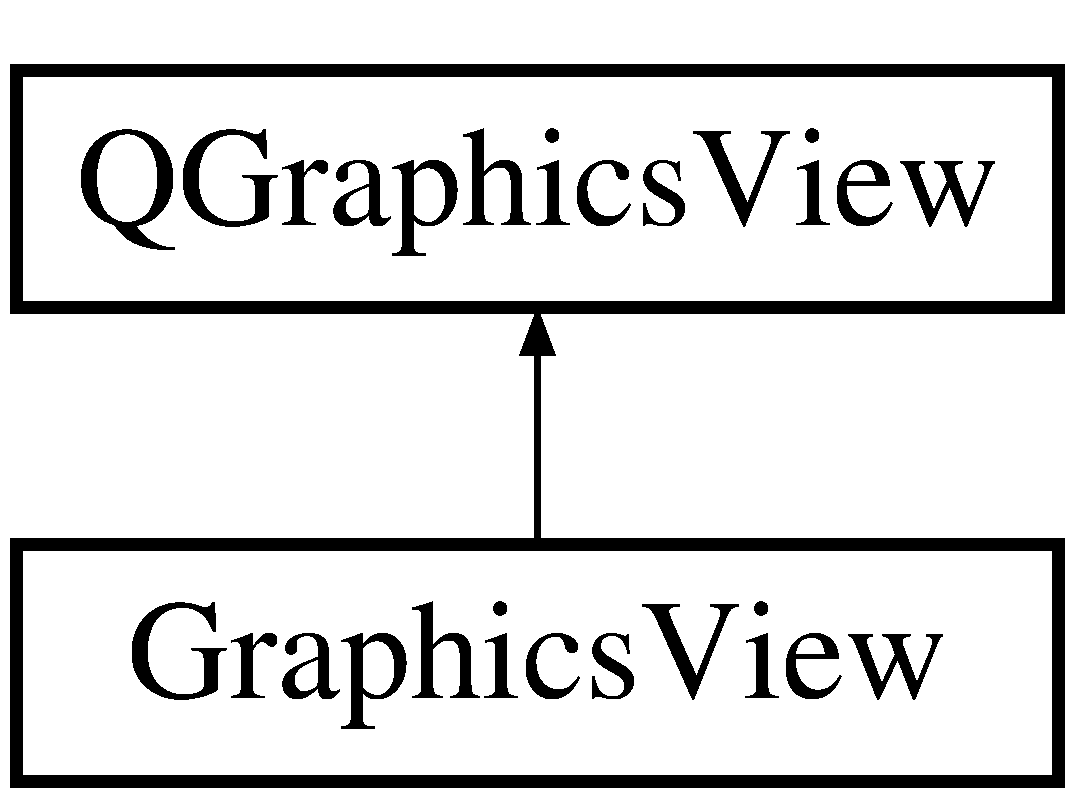
\includegraphics[height=2.000000cm]{class_graphics_view}
\end{center}
\end{figure}
\subsection*{Public Slots}
\begin{DoxyCompactItemize}
\item 
\hypertarget{class_graphics_view_a8b2bf57348fb440f8112234d5a262787}{void {\bfseries slot\-\_\-scene1} ()}\label{class_graphics_view_a8b2bf57348fb440f8112234d5a262787}

\item 
\hypertarget{class_graphics_view_a36e99b02703b60e0dd1b58c77fae2c05}{void {\bfseries slot\-\_\-scene2} ()}\label{class_graphics_view_a36e99b02703b60e0dd1b58c77fae2c05}

\item 
\hypertarget{class_graphics_view_a1a35e4c18431b529629fa51b0d4fed97}{void {\bfseries slot\-\_\-scene3} ()}\label{class_graphics_view_a1a35e4c18431b529629fa51b0d4fed97}

\item 
\hypertarget{class_graphics_view_a5afe973b24faa1b72476599bc70eedd7}{void {\bfseries slot\-\_\-scene4} ()}\label{class_graphics_view_a5afe973b24faa1b72476599bc70eedd7}

\end{DoxyCompactItemize}
\subsection*{Public Member Functions}
\begin{DoxyCompactItemize}
\item 
\hypertarget{class_graphics_view_a3704e176eba4e8036647eb85395569ff}{{\bfseries Graphics\-View} (Q\-Widget $\ast$parent=0)}\label{class_graphics_view_a3704e176eba4e8036647eb85395569ff}

\end{DoxyCompactItemize}
\subsection*{Public Attributes}
\begin{DoxyCompactItemize}
\item 
\hypertarget{class_graphics_view_acf2fdc6e6bb10767165fed1e142655de}{Q\-Graphics\-Scene {\bfseries scene}}\label{class_graphics_view_acf2fdc6e6bb10767165fed1e142655de}

\end{DoxyCompactItemize}


The documentation for this class was generated from the following files\-:\begin{DoxyCompactItemize}
\item 
graphicsview.\-h\item 
graphicsview.\-cpp\end{DoxyCompactItemize}

\hypertarget{class_hookslash}{\section{Hookslash Class Reference}
\label{class_hookslash}\index{Hookslash@{Hookslash}}
}
Inheritance diagram for Hookslash\-:\begin{figure}[H]
\begin{center}
\leavevmode
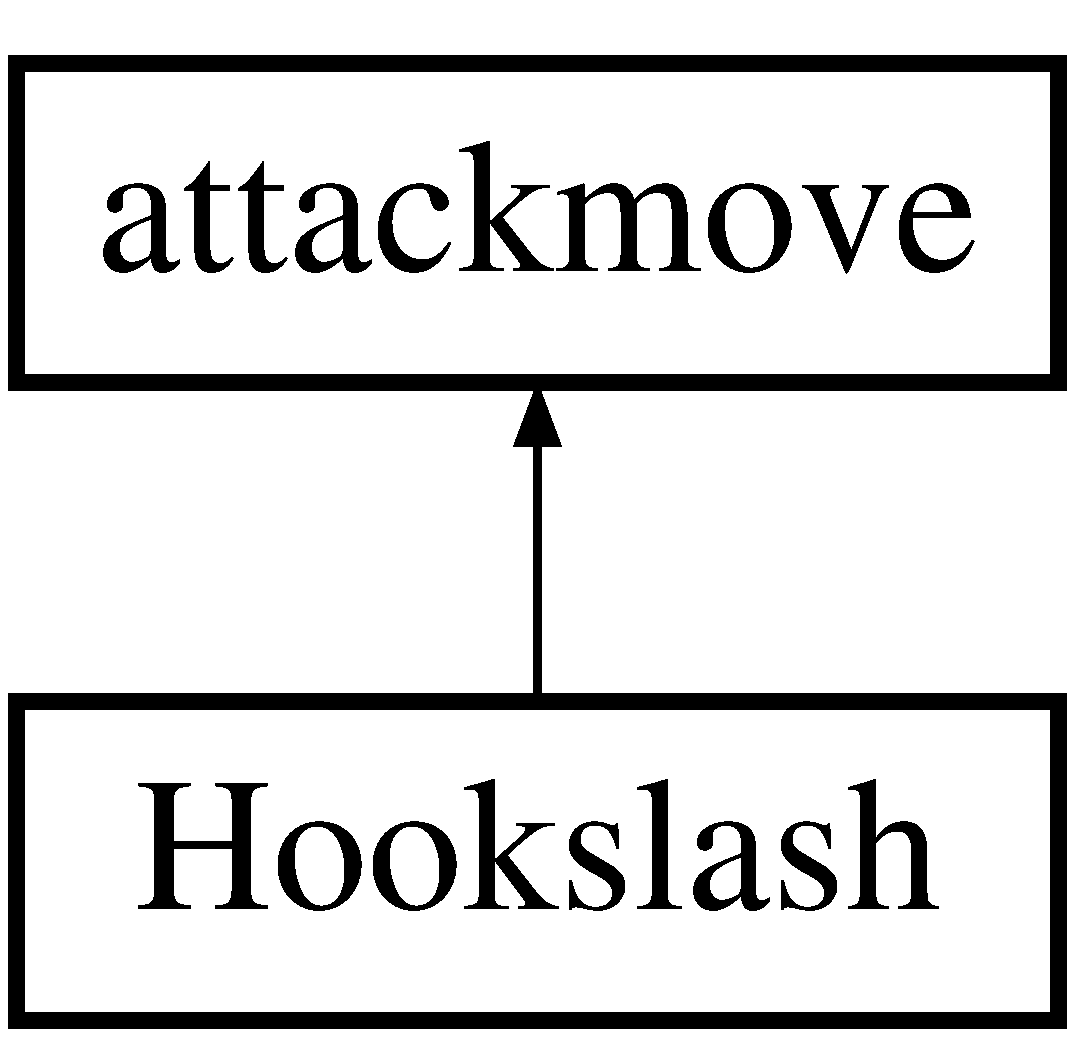
\includegraphics[height=2.000000cm]{class_hookslash}
\end{center}
\end{figure}
\subsection*{Public Member Functions}
\begin{DoxyCompactItemize}
\item 
\hypertarget{class_hookslash_a70ac467f48108a4fe26e4db666b217f8}{{\bfseries Hookslash} (int dam)}\label{class_hookslash_a70ac467f48108a4fe26e4db666b217f8}

\item 
virtual Q\-String \hyperlink{class_hookslash_aaf31aabb624b138d98f3c94fe1c37fcc}{get\-String} ()
\begin{DoxyCompactList}\small\item\em \hyperlink{classattackmove_ada49eedf4b893372c576edd48fe73161}{attackmove\-::get\-String} \end{DoxyCompactList}\item 
virtual Q\-Image \hyperlink{class_hookslash_a65c6e01ac90d1f01139dd08b93aeaa0a}{get\-Image} ()
\begin{DoxyCompactList}\small\item\em \hyperlink{classattackmove_aca59a2343b7a6c195d300dda5c8d952d}{attackmove\-::get\-Image} \end{DoxyCompactList}\item 
virtual void \hyperlink{class_hookslash_ab6a6ca9582c4d8dad26b481292bca6a0}{get\-Hover} (int hpanel, \hyperlink{class_enemy}{Enemy} $\ast$Enemies\mbox{[}3\mbox{]}, \hyperlink{classanim_items}{anim\-Items} $\ast$anim)
\begin{DoxyCompactList}\small\item\em \hyperlink{classattackmove_a0ff82349551bd72f4d57b3367bb318fa}{attackmove\-::get\-Hover} \end{DoxyCompactList}\item 
\hypertarget{class_hookslash_a704f02d57c898d1256c260218fe5c359}{virtual void {\bfseries do\-Attack} (int hpanel, \hyperlink{class_enemy}{Enemy} $\ast$Enemies\mbox{[}$\,$\mbox{]}, \hyperlink{classanim_items}{anim\-Items} $\ast$anim)}\label{class_hookslash_a704f02d57c898d1256c260218fe5c359}

\end{DoxyCompactItemize}
\subsection*{Additional Inherited Members}


\subsection{Member Function Documentation}
\hypertarget{class_hookslash_ab6a6ca9582c4d8dad26b481292bca6a0}{\index{Hookslash@{Hookslash}!get\-Hover@{get\-Hover}}
\index{get\-Hover@{get\-Hover}!Hookslash@{Hookslash}}
\subsubsection[{get\-Hover}]{\setlength{\rightskip}{0pt plus 5cm}void Hookslash\-::get\-Hover (
\begin{DoxyParamCaption}
\item[{int}]{hpanel, }
\item[{{\bf Enemy} $\ast$}]{Enemies\mbox{[}3\mbox{]}, }
\item[{{\bf anim\-Items} $\ast$}]{anim}
\end{DoxyParamCaption}
)\hspace{0.3cm}{\ttfamily [virtual]}}}\label{class_hookslash_ab6a6ca9582c4d8dad26b481292bca6a0}


\hyperlink{classattackmove_a0ff82349551bd72f4d57b3367bb318fa}{attackmove\-::get\-Hover} 


\begin{DoxyParams}{Parameters}
{\em hpanel} & \\
\hline
{\em Enemies} & \\
\hline
{\em anim} & \\
\hline
\end{DoxyParams}


Reimplemented from \hyperlink{classattackmove_a0ff82349551bd72f4d57b3367bb318fa}{attackmove}.

\hypertarget{class_hookslash_a65c6e01ac90d1f01139dd08b93aeaa0a}{\index{Hookslash@{Hookslash}!get\-Image@{get\-Image}}
\index{get\-Image@{get\-Image}!Hookslash@{Hookslash}}
\subsubsection[{get\-Image}]{\setlength{\rightskip}{0pt plus 5cm}Q\-Image Hookslash\-::get\-Image (
\begin{DoxyParamCaption}
{}
\end{DoxyParamCaption}
)\hspace{0.3cm}{\ttfamily [virtual]}}}\label{class_hookslash_a65c6e01ac90d1f01139dd08b93aeaa0a}


\hyperlink{classattackmove_aca59a2343b7a6c195d300dda5c8d952d}{attackmove\-::get\-Image} 

\begin{DoxyReturn}{Returns}

\end{DoxyReturn}


Reimplemented from \hyperlink{classattackmove_aca59a2343b7a6c195d300dda5c8d952d}{attackmove}.

\hypertarget{class_hookslash_aaf31aabb624b138d98f3c94fe1c37fcc}{\index{Hookslash@{Hookslash}!get\-String@{get\-String}}
\index{get\-String@{get\-String}!Hookslash@{Hookslash}}
\subsubsection[{get\-String}]{\setlength{\rightskip}{0pt plus 5cm}Q\-String Hookslash\-::get\-String (
\begin{DoxyParamCaption}
{}
\end{DoxyParamCaption}
)\hspace{0.3cm}{\ttfamily [virtual]}}}\label{class_hookslash_aaf31aabb624b138d98f3c94fe1c37fcc}


\hyperlink{classattackmove_ada49eedf4b893372c576edd48fe73161}{attackmove\-::get\-String} 

\begin{DoxyReturn}{Returns}
string of name, implemented in all inheritences includes damage 
\end{DoxyReturn}


Reimplemented from \hyperlink{classattackmove_ada49eedf4b893372c576edd48fe73161}{attackmove}.



The documentation for this class was generated from the following files\-:\begin{DoxyCompactItemize}
\item 
hookslash.\-h\item 
hookslash.\-cpp\end{DoxyCompactItemize}

\hypertarget{class_hunter}{\section{Hunter Class Reference}
\label{class_hunter}\index{Hunter@{Hunter}}
}
Inheritance diagram for Hunter\-:\begin{figure}[H]
\begin{center}
\leavevmode
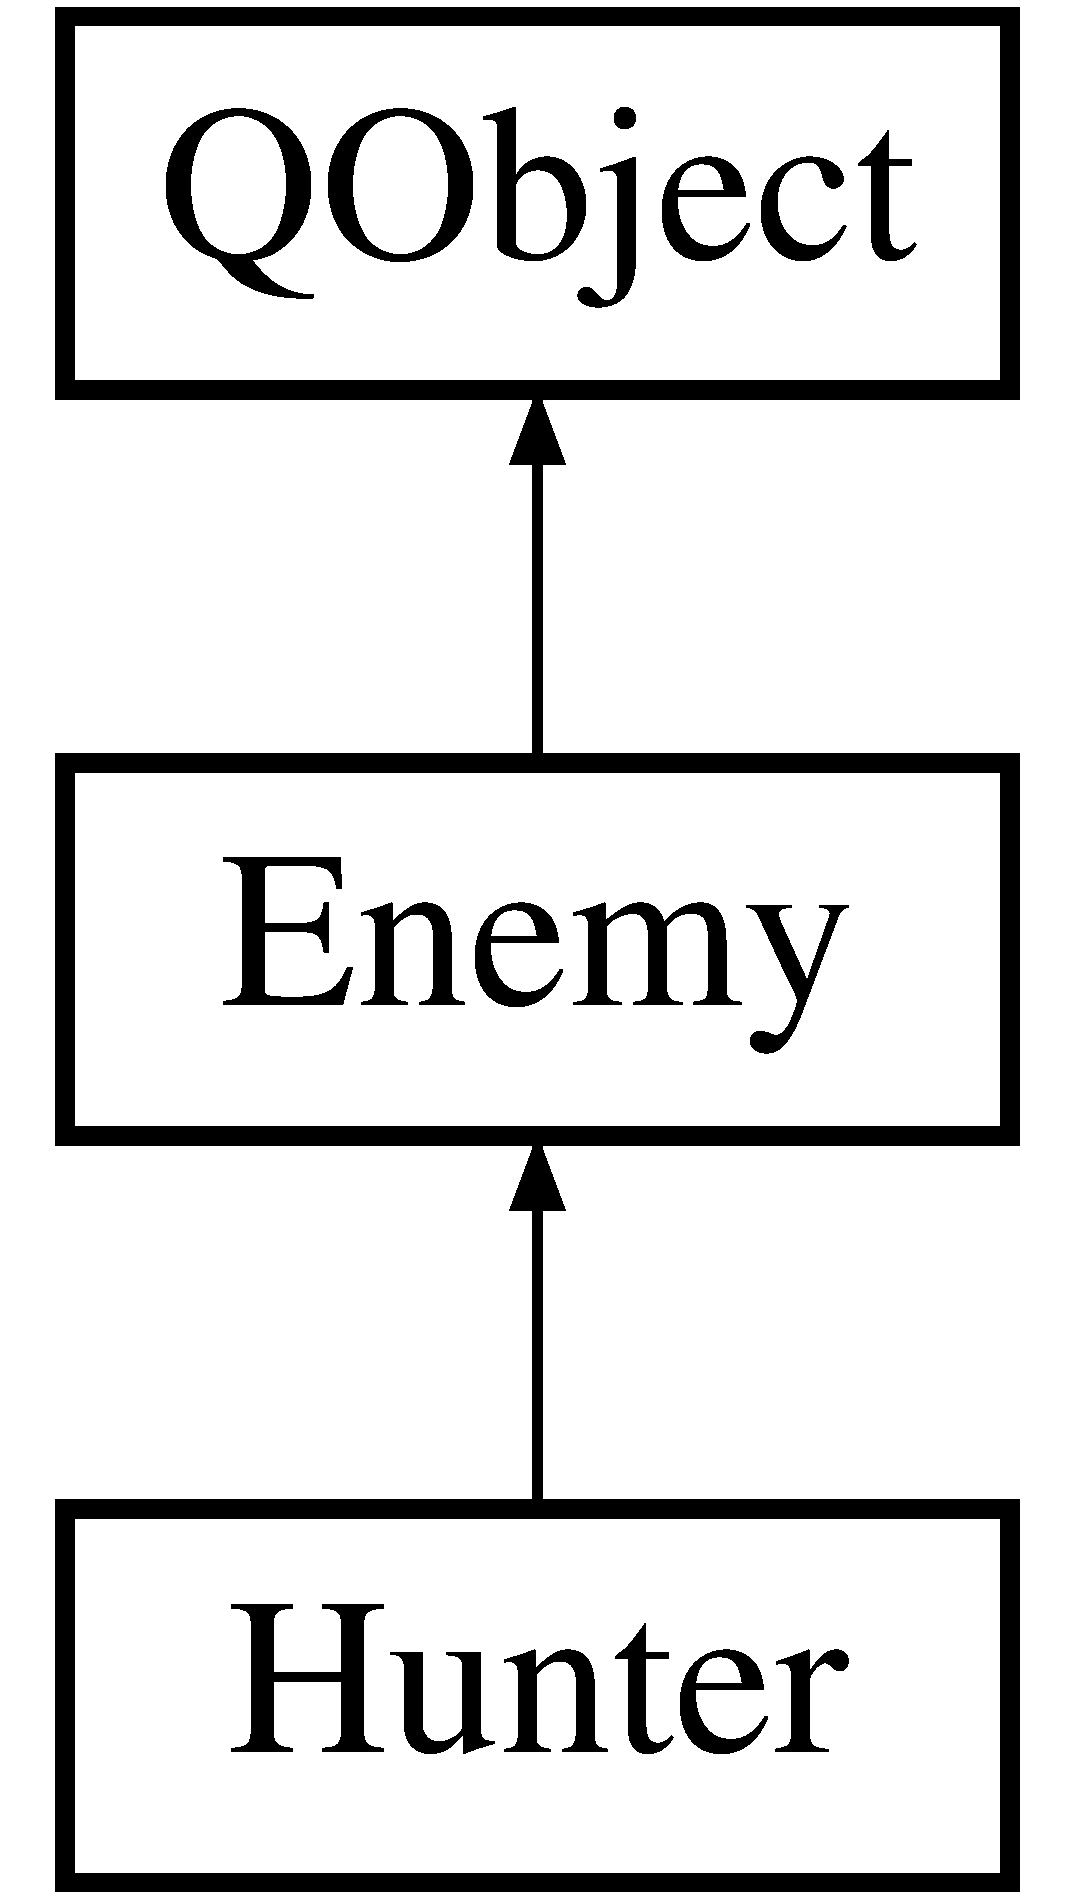
\includegraphics[height=3.000000cm]{class_hunter}
\end{center}
\end{figure}
\subsection*{Public Member Functions}
\begin{DoxyCompactItemize}
\item 
\hypertarget{class_hunter_a6516ea26662db6188fa2102ae768eca2}{{\bfseries Hunter} (int clev, int cx, int cy, bool cup)}\label{class_hunter_a6516ea26662db6188fa2102ae768eca2}

\item 
virtual void \hyperlink{class_hunter_a910f2c34961a3d7fb1caa91e65b5d743}{do\-Turn} (\hyperlink{class_character}{Character} $\ast$Hero)
\begin{DoxyCompactList}\small\item\em \hyperlink{class_enemy_a56e4b9b07e8cd2a4e5ecfa8ff5b9265a}{Enemy\-::do\-Turn} based on hero's panel, does it's move. \end{DoxyCompactList}\item 
\hypertarget{class_hunter_adc1727098c026b726430a638d4536970}{bool {\bfseries get\-Lef} ()}\label{class_hunter_adc1727098c026b726430a638d4536970}

\item 
\hypertarget{class_hunter_ac1cb95a730a5af30d4fe50b1ff296696}{void {\bfseries set\-Lef} (bool clef)}\label{class_hunter_ac1cb95a730a5af30d4fe50b1ff296696}

\item 
\hypertarget{class_hunter_a407e130c2e904630fd501c329eaeac77}{virtual Q\-Image {\bfseries get\-Pic} ()}\label{class_hunter_a407e130c2e904630fd501c329eaeac77}

\item 
virtual void \hyperlink{class_hunter_a765f282edf2fd27998740d33ed81a423}{draw\-Self} (Q\-Painter $\ast$g, int gx, int gy)
\begin{DoxyCompactList}\small\item\em \hyperlink{class_enemy_a3251244e8e7ac657687d6be5a8da71bb}{Enemy\-::draw\-Self} draws itself using painter, includes title and hp. \end{DoxyCompactList}\end{DoxyCompactItemize}
\subsection*{Additional Inherited Members}


\subsection{Member Function Documentation}
\hypertarget{class_hunter_a910f2c34961a3d7fb1caa91e65b5d743}{\index{Hunter@{Hunter}!do\-Turn@{do\-Turn}}
\index{do\-Turn@{do\-Turn}!Hunter@{Hunter}}
\subsubsection[{do\-Turn}]{\setlength{\rightskip}{0pt plus 5cm}void Hunter\-::do\-Turn (
\begin{DoxyParamCaption}
\item[{{\bf Character} $\ast$}]{Hero}
\end{DoxyParamCaption}
)\hspace{0.3cm}{\ttfamily [virtual]}}}\label{class_hunter_a910f2c34961a3d7fb1caa91e65b5d743}


\hyperlink{class_enemy_a56e4b9b07e8cd2a4e5ecfa8ff5b9265a}{Enemy\-::do\-Turn} based on hero's panel, does it's move. 


\begin{DoxyParams}{Parameters}
{\em Hero} & \\
\hline
\end{DoxyParams}


Reimplemented from \hyperlink{class_enemy_a56e4b9b07e8cd2a4e5ecfa8ff5b9265a}{Enemy}.

\hypertarget{class_hunter_a765f282edf2fd27998740d33ed81a423}{\index{Hunter@{Hunter}!draw\-Self@{draw\-Self}}
\index{draw\-Self@{draw\-Self}!Hunter@{Hunter}}
\subsubsection[{draw\-Self}]{\setlength{\rightskip}{0pt plus 5cm}void Hunter\-::draw\-Self (
\begin{DoxyParamCaption}
\item[{Q\-Painter $\ast$}]{g, }
\item[{int}]{gx, }
\item[{int}]{gy}
\end{DoxyParamCaption}
)\hspace{0.3cm}{\ttfamily [virtual]}}}\label{class_hunter_a765f282edf2fd27998740d33ed81a423}


\hyperlink{class_enemy_a3251244e8e7ac657687d6be5a8da71bb}{Enemy\-::draw\-Self} draws itself using painter, includes title and hp. 


\begin{DoxyParams}{Parameters}
{\em g} & \\
\hline
{\em gx} & \\
\hline
{\em gy} & \\
\hline
\end{DoxyParams}


Reimplemented from \hyperlink{class_enemy_a3251244e8e7ac657687d6be5a8da71bb}{Enemy}.



The documentation for this class was generated from the following files\-:\begin{DoxyCompactItemize}
\item 
hunter.\-h\item 
hunter.\-cpp\end{DoxyCompactItemize}

\hypertarget{class_in_store}{\section{In\-Store Class Reference}
\label{class_in_store}\index{In\-Store@{In\-Store}}
}
Inheritance diagram for In\-Store\-:\begin{figure}[H]
\begin{center}
\leavevmode
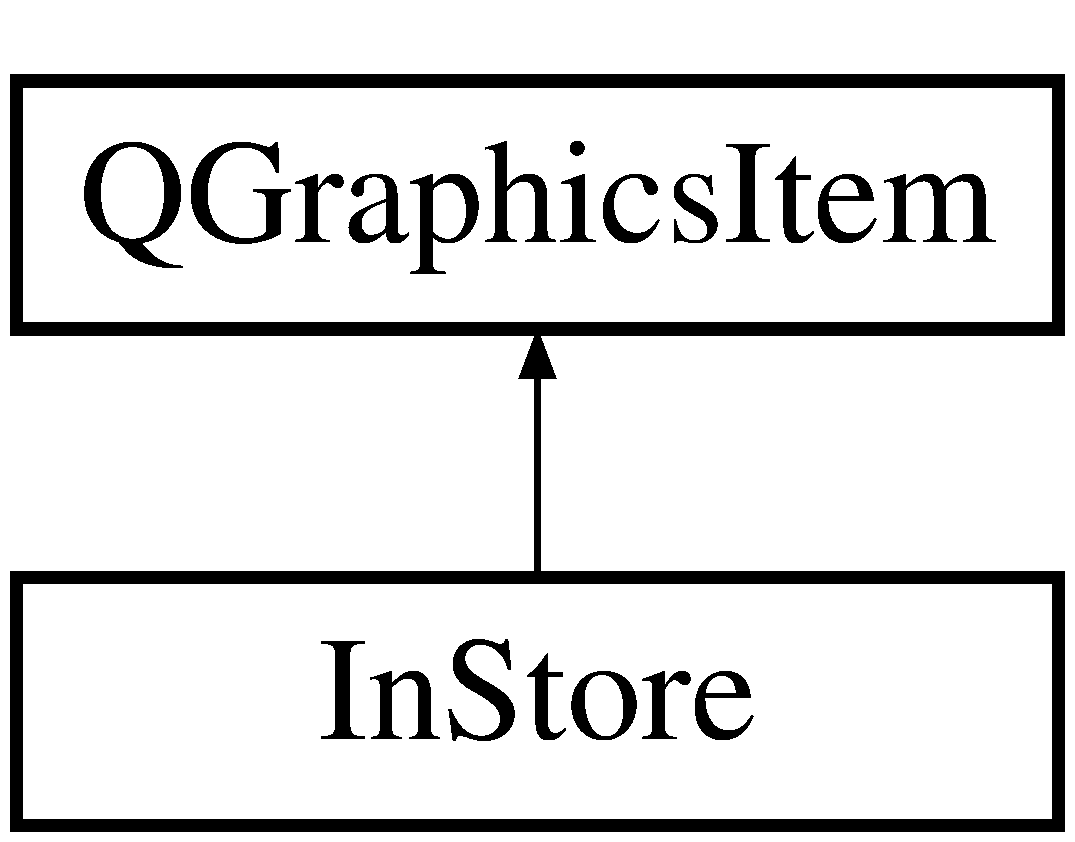
\includegraphics[height=2.000000cm]{class_in_store}
\end{center}
\end{figure}
\subsection*{Public Member Functions}
\begin{DoxyCompactItemize}
\item 
\hypertarget{class_in_store_ada28f501479c707689eeb14d5258c11b}{{\bfseries In\-Store} (Q\-Graphics\-Item $\ast$parent=N\-U\-L\-L)}\label{class_in_store_ada28f501479c707689eeb14d5258c11b}

\item 
\hypertarget{class_in_store_a7778b31865d65ce049dda2bf73569962}{void {\bfseries paint} (Q\-Painter $\ast$painter, const Q\-Style\-Option\-Graphics\-Item $\ast$option, Q\-Widget $\ast$widget)}\label{class_in_store_a7778b31865d65ce049dda2bf73569962}

\end{DoxyCompactItemize}
\subsection*{Protected Member Functions}
\begin{DoxyCompactItemize}
\item 
\hypertarget{class_in_store_a00c8b6bd40d5d7580e52418b5e58d9ef}{Q\-Rect\-F {\bfseries bounding\-Rect} () const }\label{class_in_store_a00c8b6bd40d5d7580e52418b5e58d9ef}

\end{DoxyCompactItemize}


The documentation for this class was generated from the following files\-:\begin{DoxyCompactItemize}
\item 
instore.\-h\item 
instore.\-cpp\end{DoxyCompactItemize}

\hypertarget{class_main_window}{\section{Main\-Window Class Reference}
\label{class_main_window}\index{Main\-Window@{Main\-Window}}
}
Inheritance diagram for Main\-Window\-:\begin{figure}[H]
\begin{center}
\leavevmode
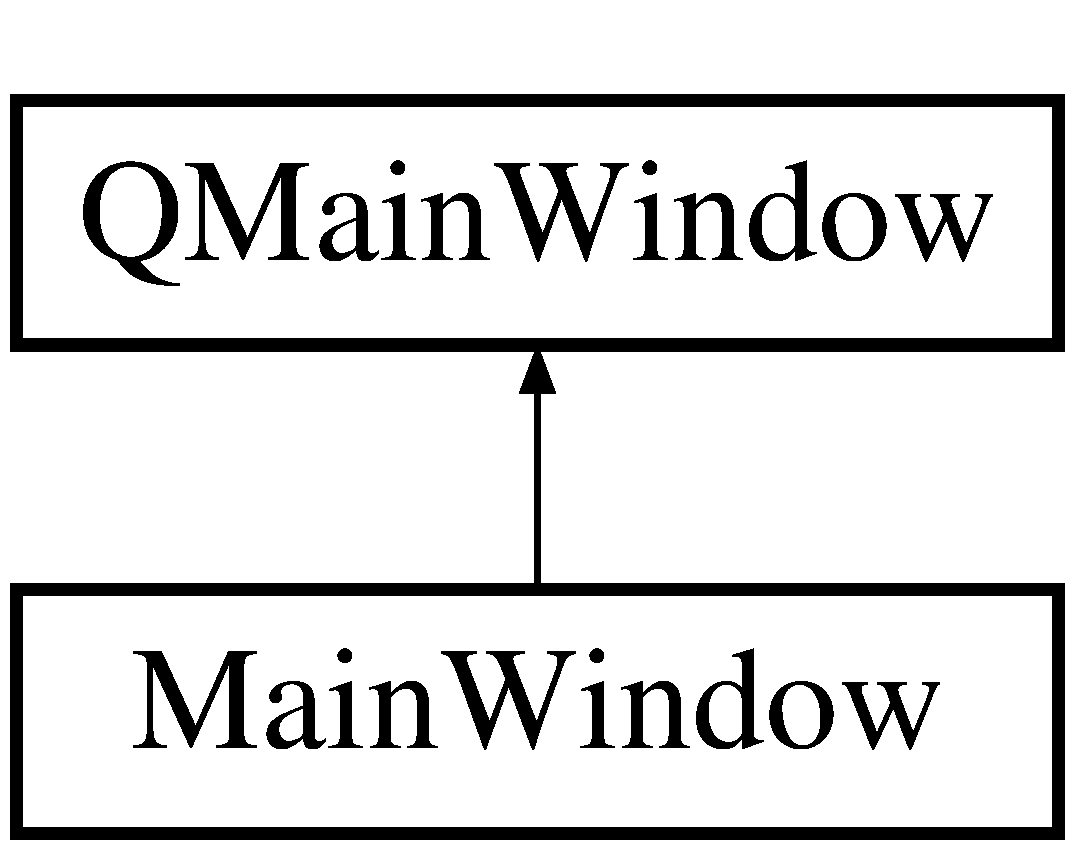
\includegraphics[height=2.000000cm]{class_main_window}
\end{center}
\end{figure}
\subsection*{Public Member Functions}
\begin{DoxyCompactItemize}
\item 
\hypertarget{class_main_window_a8b244be8b7b7db1b08de2a2acb9409db}{{\bfseries Main\-Window} (Q\-Widget $\ast$parent=0)}\label{class_main_window_a8b244be8b7b7db1b08de2a2acb9409db}

\end{DoxyCompactItemize}


The documentation for this class was generated from the following files\-:\begin{DoxyCompactItemize}
\item 
mainwindow.\-h\item 
mainwindow.\-cpp\end{DoxyCompactItemize}

\hypertarget{class_ui_1_1_main_window}{\section{Ui\-:\-:Main\-Window Class Reference}
\label{class_ui_1_1_main_window}\index{Ui\-::\-Main\-Window@{Ui\-::\-Main\-Window}}
}
Inheritance diagram for Ui\-:\-:Main\-Window\-:\begin{figure}[H]
\begin{center}
\leavevmode
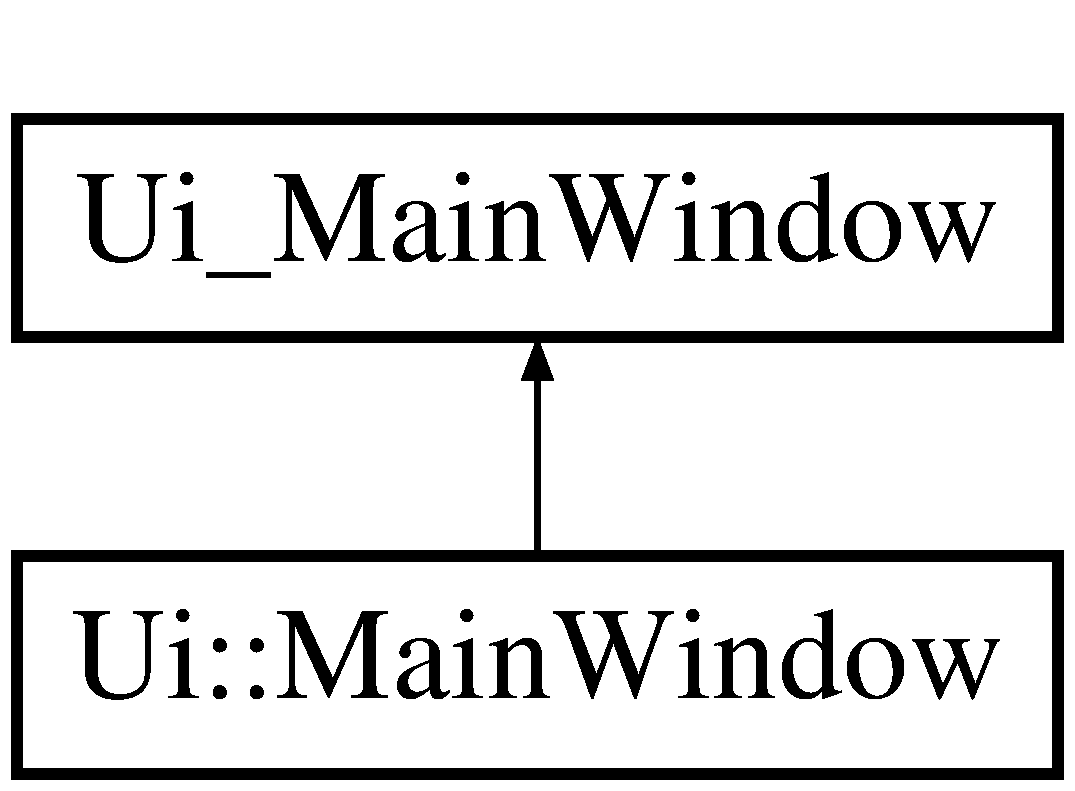
\includegraphics[height=2.000000cm]{class_ui_1_1_main_window}
\end{center}
\end{figure}
\subsection*{Additional Inherited Members}


The documentation for this class was generated from the following file\-:\begin{DoxyCompactItemize}
\item 
ui\-\_\-mainwindow.\-h\end{DoxyCompactItemize}

\hypertarget{class_map_enemy}{\section{Map\-Enemy Class Reference}
\label{class_map_enemy}\index{Map\-Enemy@{Map\-Enemy}}
}
Inheritance diagram for Map\-Enemy\-:\begin{figure}[H]
\begin{center}
\leavevmode
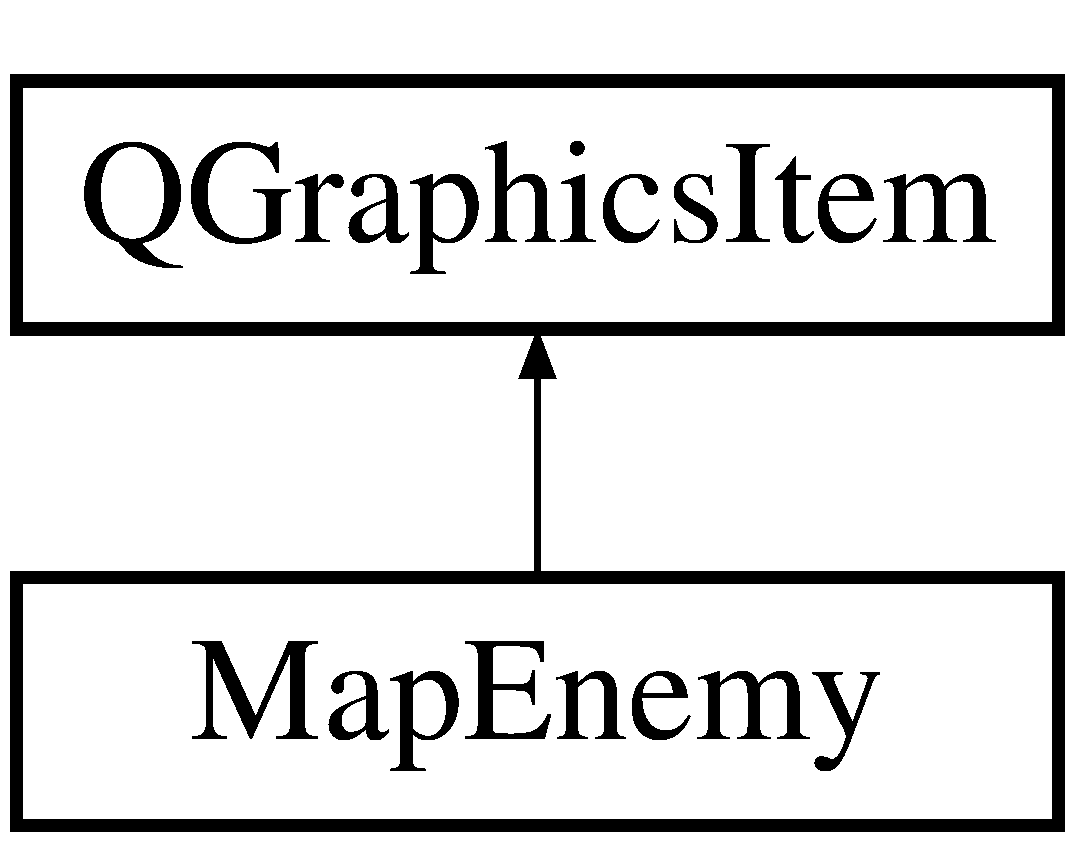
\includegraphics[height=2.000000cm]{class_map_enemy}
\end{center}
\end{figure}
\subsection*{Public Member Functions}
\begin{DoxyCompactItemize}
\item 
\hyperlink{class_map_enemy_a0ec0658d11120c1618bdd39fae1c8f30}{Map\-Enemy} (Q\-Graphics\-Item $\ast$parent=N\-U\-L\-L)
\begin{DoxyCompactList}\small\item\em An enemy item constructor. \end{DoxyCompactList}\item 
\hypertarget{class_map_enemy_ae67d6517d65f658fb08b66ced225e421}{\hyperlink{class_map_enemy_ae67d6517d65f658fb08b66ced225e421}{$\sim$\-Map\-Enemy} ()}\label{class_map_enemy_ae67d6517d65f658fb08b66ced225e421}

\begin{DoxyCompactList}\small\item\em calls to the destruction of the enemy item. \end{DoxyCompactList}\end{DoxyCompactItemize}
\subsection*{Protected Member Functions}
\begin{DoxyCompactItemize}
\item 
void \hyperlink{class_map_enemy_a824c6d66bce423f3e89fe4111a9cf2f0}{paint} (Q\-Painter $\ast$painter, const Q\-Style\-Option\-Graphics\-Item $\ast$option, Q\-Widget $\ast$widget)
\begin{DoxyCompactList}\small\item\em Paints the enemy. \end{DoxyCompactList}\item 
Q\-Rect\-F \hyperlink{class_map_enemy_ae8847f947b045ae9fd3c1fd7ccb522fc}{bounding\-Rect} () const 
\begin{DoxyCompactList}\small\item\em \hyperlink{class_map_enemy_ae8847f947b045ae9fd3c1fd7ccb522fc}{Map\-Enemy\-::bounding\-Rect} is used to set a bounding rect. \end{DoxyCompactList}\item 
\hypertarget{class_map_enemy_a8b41e9638d4c20b9480b6e1130510bf8}{virtual void \hyperlink{class_map_enemy_a8b41e9638d4c20b9480b6e1130510bf8}{collision\-Event} ()}\label{class_map_enemy_a8b41e9638d4c20b9480b6e1130510bf8}

\begin{DoxyCompactList}\small\item\em not used, since all events happened on the hero's side. He collides and all respond. \end{DoxyCompactList}\end{DoxyCompactItemize}


\subsection{Constructor \& Destructor Documentation}
\hypertarget{class_map_enemy_a0ec0658d11120c1618bdd39fae1c8f30}{\index{Map\-Enemy@{Map\-Enemy}!Map\-Enemy@{Map\-Enemy}}
\index{Map\-Enemy@{Map\-Enemy}!MapEnemy@{Map\-Enemy}}
\subsubsection[{Map\-Enemy}]{\setlength{\rightskip}{0pt plus 5cm}Map\-Enemy\-::\-Map\-Enemy (
\begin{DoxyParamCaption}
\item[{Q\-Graphics\-Item $\ast$}]{parent = {\ttfamily NULL}}
\end{DoxyParamCaption}
)}}\label{class_map_enemy_a0ec0658d11120c1618bdd39fae1c8f30}


An enemy item constructor. 


\begin{DoxyParams}{Parameters}
{\em parent} & \\
\hline
\end{DoxyParams}


\subsection{Member Function Documentation}
\hypertarget{class_map_enemy_ae8847f947b045ae9fd3c1fd7ccb522fc}{\index{Map\-Enemy@{Map\-Enemy}!bounding\-Rect@{bounding\-Rect}}
\index{bounding\-Rect@{bounding\-Rect}!MapEnemy@{Map\-Enemy}}
\subsubsection[{bounding\-Rect}]{\setlength{\rightskip}{0pt plus 5cm}Q\-Rect\-F Map\-Enemy\-::bounding\-Rect (
\begin{DoxyParamCaption}
{}
\end{DoxyParamCaption}
) const\hspace{0.3cm}{\ttfamily [protected]}}}\label{class_map_enemy_ae8847f947b045ae9fd3c1fd7ccb522fc}


\hyperlink{class_map_enemy_ae8847f947b045ae9fd3c1fd7ccb522fc}{Map\-Enemy\-::bounding\-Rect} is used to set a bounding rect. 

\begin{DoxyReturn}{Returns}
Q\-Rect\-F, the bounding rect of the item 
\end{DoxyReturn}
\hypertarget{class_map_enemy_a824c6d66bce423f3e89fe4111a9cf2f0}{\index{Map\-Enemy@{Map\-Enemy}!paint@{paint}}
\index{paint@{paint}!MapEnemy@{Map\-Enemy}}
\subsubsection[{paint}]{\setlength{\rightskip}{0pt plus 5cm}void Map\-Enemy\-::paint (
\begin{DoxyParamCaption}
\item[{Q\-Painter $\ast$}]{painter, }
\item[{const Q\-Style\-Option\-Graphics\-Item $\ast$}]{option, }
\item[{Q\-Widget $\ast$}]{widget}
\end{DoxyParamCaption}
)\hspace{0.3cm}{\ttfamily [protected]}}}\label{class_map_enemy_a824c6d66bce423f3e89fe4111a9cf2f0}


Paints the enemy. 


\begin{DoxyParams}{Parameters}
{\em painter} & \\
\hline
{\em option} & \\
\hline
{\em widget} & \\
\hline
\end{DoxyParams}


The documentation for this class was generated from the following files\-:\begin{DoxyCompactItemize}
\item 
mapenemy.\-h\item 
mapenemy.\-cpp\end{DoxyCompactItemize}

\hypertarget{class_map_hero}{\section{Map\-Hero Class Reference}
\label{class_map_hero}\index{Map\-Hero@{Map\-Hero}}
}
Inheritance diagram for Map\-Hero\-:\begin{figure}[H]
\begin{center}
\leavevmode
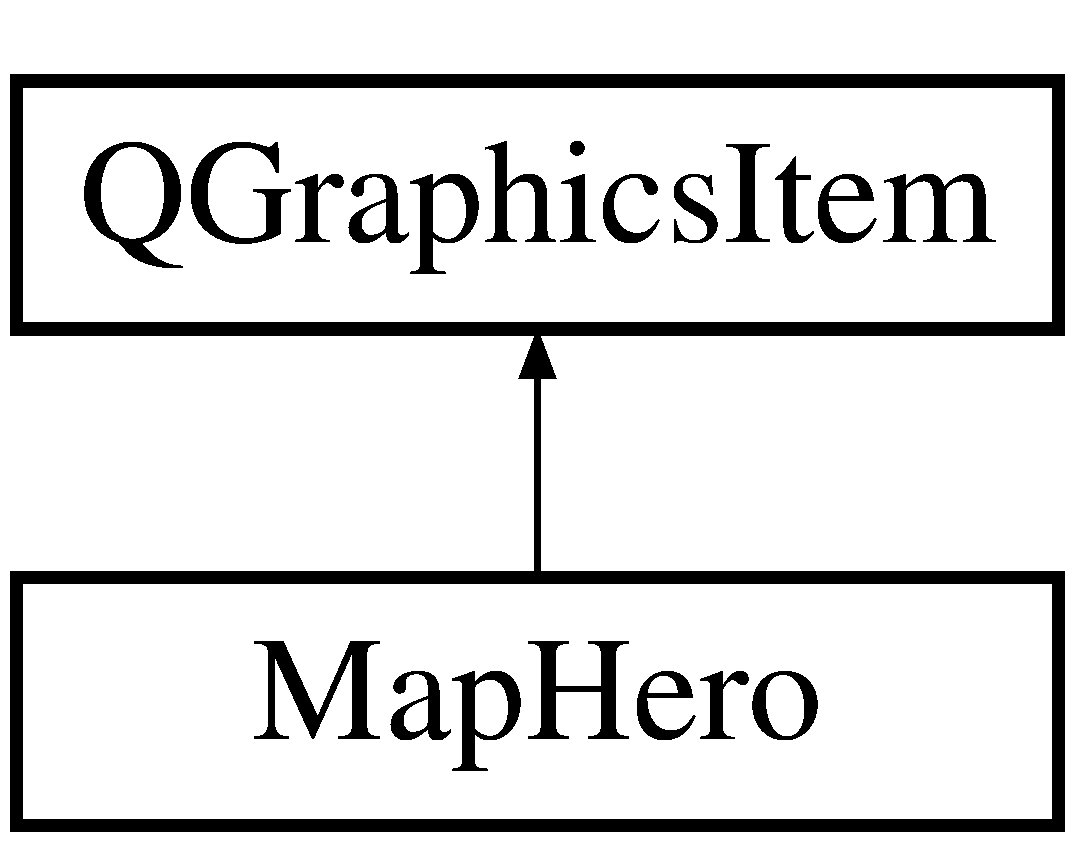
\includegraphics[height=2.000000cm]{class_map_hero}
\end{center}
\end{figure}
\subsection*{Public Member Functions}
\begin{DoxyCompactItemize}
\item 
\hyperlink{class_map_hero_aa5dd4f5162b14b9c4dca9fe6b53482bd}{Map\-Hero} (Q\-Graphics\-Item $\ast$parent=0)
\begin{DoxyCompactList}\small\item\em Constructor for the Map Hero, the most awesomest and fanciful part of the map section of the program. Basically does everything for itself. \end{DoxyCompactList}\item 
void \hyperlink{class_map_hero_adb1c259574dc015f4f12055cced7508e}{point\-To\-Enemy} (\hyperlink{class_map_enemy}{Map\-Enemy} $\ast$enemy, \hyperlink{class_mini_enemy}{Mini\-Enemy} $\ast$mini\-Enemy, \hyperlink{class_mega_enemy}{Mega\-Enemy} $\ast$mega\-Enemy)
\begin{DoxyCompactList}\small\item\em Gives me enemy pointers, so hero can set appropriate actions onto the screen. \end{DoxyCompactList}\item 
void \hyperlink{class_map_hero_aa391ed82ab55cef8a3ec726cf89cac68}{point\-To\-Store} (\hyperlink{class_to_store}{To\-Store} $\ast$storay)
\begin{DoxyCompactList}\small\item\em gets a pointer to the store \end{DoxyCompactList}\item 
void \hyperlink{class_map_hero_a7d9e977eff02971c7899d1de134b598e}{point\-To\-Me} (\hyperlink{class_map_hero}{Map\-Hero} $\ast$hera)
\begin{DoxyCompactList}\small\item\em pointer to self. \end{DoxyCompactList}\item 
void \hyperlink{class_map_hero_aa931db713b67c5e65989a667ab6048dc}{point\-To\-In\-Store} (\hyperlink{class_in_store}{In\-Store} $\ast$in\-Storay)
\begin{DoxyCompactList}\small\item\em pointer to go in store. \end{DoxyCompactList}\item 
void \hyperlink{class_map_hero_aa6fa52a5f93d4d38fb6a331b0b74cb5d}{point\-To\-End} (\hyperlink{class_to_end}{To\-End} $\ast$to\-End)
\begin{DoxyCompactList}\small\item\em points to the pointer that sends you to the last level. \end{DoxyCompactList}\item 
void \hyperlink{class_map_hero_ab1afb3bc50f4e64557d93d9e5933de55}{point\-From\-In\-Store} (\hyperlink{class_back_from_in_store}{Back\-From\-In\-Store} $\ast$from\-In\-Store)
\begin{DoxyCompactList}\small\item\em stores a pointer to the map from in store. \end{DoxyCompactList}\item 
void \hyperlink{class_map_hero_a2cc42c31942ce242e9bbcdefe29c6d8b}{point\-From\-Store} (\hyperlink{class_back_from_store}{Back\-From\-Store} $\ast$from\-Store)
\begin{DoxyCompactList}\small\item\em this is a functino that returns a pointer to the hero set to the store map scene. \end{DoxyCompactList}\item 
void \hyperlink{class_map_hero_a6c0c09301c2af7d8513d089f4af1081f}{point\-From\-End} (\hyperlink{class_back_from_end}{Back\-From\-End} $\ast$from\-End)
\begin{DoxyCompactList}\small\item\em stores a pointer to the end from the \end{DoxyCompactList}\item 
void \hyperlink{class_map_hero_a041511fb2146b7362ae6aa61637eba4c}{get\-Graphics\-View} (Q\-Graphics\-View $\ast$graphs)
\begin{DoxyCompactList}\small\item\em \hyperlink{class_map_hero_a041511fb2146b7362ae6aa61637eba4c}{Map\-Hero\-::get\-Graphics\-View}. \end{DoxyCompactList}\item 
void \hyperlink{class_map_hero_a2bee96b4db60849c9313ca7d0f3432c4}{get\-Graphics\-Scene} (Q\-Graphics\-Scene $\ast$begs, Q\-Graphics\-Scene $\ast$mids, Q\-Graphics\-Scene $\ast$ends, Q\-Graphics\-Scene $\ast$stores)
\begin{DoxyCompactList}\small\item\em \hyperlink{class_map_hero_a2bee96b4db60849c9313ca7d0f3432c4}{Map\-Hero\-::get\-Graphics\-Scene}. \end{DoxyCompactList}\end{DoxyCompactItemize}
\subsection*{Public Attributes}
\begin{DoxyCompactItemize}
\item 
\hypertarget{class_map_hero_ab072656adab893fda581db0ceeb2cba6}{\hyperlink{class_pause}{Pause} $\ast$ {\bfseries pause}}\label{class_map_hero_ab072656adab893fda581db0ceeb2cba6}

\item 
\hypertarget{class_map_hero_a130f5008f4e8b74f51d7a109bb870322}{\hyperlink{class_map_enemy}{Map\-Enemy} $\ast$ {\bfseries enemon}}\label{class_map_hero_a130f5008f4e8b74f51d7a109bb870322}

\item 
\hypertarget{class_map_hero_a022d2451554c6c21d13a058c2648716b}{\hyperlink{class_mini_enemy}{Mini\-Enemy} $\ast$ {\bfseries minemy}}\label{class_map_hero_a022d2451554c6c21d13a058c2648716b}

\item 
\hypertarget{class_map_hero_ac530f7cced8f11a975f57c8ae17fde9f}{\hyperlink{class_mega_enemy}{Mega\-Enemy} $\ast$ {\bfseries menemy}}\label{class_map_hero_ac530f7cced8f11a975f57c8ae17fde9f}

\item 
\hypertarget{class_map_hero_a2a7b5b4cc3fd5ae5e1ca5b8439799a45}{\hyperlink{class_to_store}{To\-Store} $\ast$ {\bfseries stora}}\label{class_map_hero_a2a7b5b4cc3fd5ae5e1ca5b8439799a45}

\item 
\hypertarget{class_map_hero_abb3ff67f6c2568f4e45f68772af7f85e}{\hyperlink{class_in_store}{In\-Store} $\ast$ {\bfseries in\-Stora}}\label{class_map_hero_abb3ff67f6c2568f4e45f68772af7f85e}

\item 
\hypertarget{class_map_hero_a0f47e89ab15b67bf50d45dd76ffb52c3}{\hyperlink{class_map_hero}{Map\-Hero} $\ast$ {\bfseries hero}}\label{class_map_hero_a0f47e89ab15b67bf50d45dd76ffb52c3}

\item 
\hypertarget{class_map_hero_ab5ce0c1d818ada72e0da5f692daf734a}{\hyperlink{class_to_end}{To\-End} $\ast$ {\bfseries m\-End}}\label{class_map_hero_ab5ce0c1d818ada72e0da5f692daf734a}

\item 
\hypertarget{class_map_hero_a08cdb7fb2e49144facebebe27e61150a}{\hyperlink{class_back_from_store}{Back\-From\-Store} $\ast$ {\bfseries o\-Store}}\label{class_map_hero_a08cdb7fb2e49144facebebe27e61150a}

\item 
\hypertarget{class_map_hero_ada2b7edb1fd66c4d88f76d5fae932ef3}{\hyperlink{class_back_from_in_store}{Back\-From\-In\-Store} $\ast$ {\bfseries o\-In\-Store}}\label{class_map_hero_ada2b7edb1fd66c4d88f76d5fae932ef3}

\item 
\hypertarget{class_map_hero_a5e2fab5d73786c73c283cdc38fa6caf4}{\hyperlink{class_back_from_end}{Back\-From\-End} $\ast$ {\bfseries o\-End}}\label{class_map_hero_a5e2fab5d73786c73c283cdc38fa6caf4}

\item 
\hypertarget{class_map_hero_a47306a29cb36d3920c78312a3c8bdbe0}{int {\bfseries hero\-Image}}\label{class_map_hero_a47306a29cb36d3920c78312a3c8bdbe0}

\item 
\hypertarget{class_map_hero_a1fc5870b5b8430c1bb63286c1f32d505}{int {\bfseries i\-Am\-In}}\label{class_map_hero_a1fc5870b5b8430c1bb63286c1f32d505}

\item 
\hypertarget{class_map_hero_a08d2d2b5fef26ba074c2bced337749d5}{int {\bfseries fo\-Min}}\label{class_map_hero_a08d2d2b5fef26ba074c2bced337749d5}

\item 
\hypertarget{class_map_hero_a557cff60685689172c8673885ad2bde3}{int {\bfseries fo\-Enem}}\label{class_map_hero_a557cff60685689172c8673885ad2bde3}

\item 
\hypertarget{class_map_hero_a93320d19f339ea368cea1492db7cd0cf}{int {\bfseries fo\-Men}}\label{class_map_hero_a93320d19f339ea368cea1492db7cd0cf}

\item 
\hypertarget{class_map_hero_afbcd09655306830d8f805798ec7c6fe9}{Q\-Graphics\-View $\ast$ {\bfseries graph}}\label{class_map_hero_afbcd09655306830d8f805798ec7c6fe9}

\item 
\hypertarget{class_map_hero_a0d54e7a305355cdb791d35e2cfcc5845}{Q\-Graphics\-Scene $\ast$ {\bfseries begin}}\label{class_map_hero_a0d54e7a305355cdb791d35e2cfcc5845}

\item 
\hypertarget{class_map_hero_a7cf484cf11c1b664b0dbb4e260fe4b34}{Q\-Graphics\-Scene $\ast$ {\bfseries mid}}\label{class_map_hero_a7cf484cf11c1b664b0dbb4e260fe4b34}

\item 
\hypertarget{class_map_hero_a6936c0a3c199c9671e6a15975dfac5ff}{Q\-Graphics\-Scene $\ast$ {\bfseries end}}\label{class_map_hero_a6936c0a3c199c9671e6a15975dfac5ff}

\item 
\hypertarget{class_map_hero_a35d4049205da1845fc125174be91fed0}{Q\-Graphics\-Scene $\ast$ {\bfseries store}}\label{class_map_hero_a35d4049205da1845fc125174be91fed0}

\item 
\hypertarget{class_map_hero_a66cef0ed826bc7a9e2861354bf6f44c3}{\hyperlink{classattackframe}{attackframe} $\ast$ {\bfseries battle}}\label{class_map_hero_a66cef0ed826bc7a9e2861354bf6f44c3}

\end{DoxyCompactItemize}
\subsection*{Protected Member Functions}
\begin{DoxyCompactItemize}
\item 
void \hyperlink{class_map_hero_a001330799c5a8c83f9689f87c0e4188e}{paint} (Q\-Painter $\ast$painter, const Q\-Style\-Option\-Graphics\-Item $\ast$option, Q\-Widget $\ast$widget)
\begin{DoxyCompactList}\small\item\em Paints the hero based on what hero image number is placed. \end{DoxyCompactList}\item 
Q\-Rect\-F \hyperlink{class_map_hero_a45109e2e0ed082a5df0ff820c9c7d5bb}{bounding\-Rect} () const 
\begin{DoxyCompactList}\small\item\em sets the bouding rect to the hero item. \end{DoxyCompactList}\item 
\hypertarget{class_map_hero_ae0a3357463f62642da708cad22f7bf4c}{virtual void \hyperlink{class_map_hero_ae0a3357463f62642da708cad22f7bf4c}{key\-Press\-Event} (Q\-Key\-Event $\ast$event)}\label{class_map_hero_ae0a3357463f62642da708cad22f7bf4c}

\begin{DoxyCompactList}\small\item\em This is where the majority of the collision is taking place. aram , is the key that is pressed. \end{DoxyCompactList}\end{DoxyCompactItemize}


\subsection{Constructor \& Destructor Documentation}
\hypertarget{class_map_hero_aa5dd4f5162b14b9c4dca9fe6b53482bd}{\index{Map\-Hero@{Map\-Hero}!Map\-Hero@{Map\-Hero}}
\index{Map\-Hero@{Map\-Hero}!MapHero@{Map\-Hero}}
\subsubsection[{Map\-Hero}]{\setlength{\rightskip}{0pt plus 5cm}Map\-Hero\-::\-Map\-Hero (
\begin{DoxyParamCaption}
\item[{Q\-Graphics\-Item $\ast$}]{parent = {\ttfamily 0}}
\end{DoxyParamCaption}
)}}\label{class_map_hero_aa5dd4f5162b14b9c4dca9fe6b53482bd}


Constructor for the Map Hero, the most awesomest and fanciful part of the map section of the program. Basically does everything for itself. 


\begin{DoxyParams}{Parameters}
{\em parent} & \\
\hline
\end{DoxyParams}


\subsection{Member Function Documentation}
\hypertarget{class_map_hero_a45109e2e0ed082a5df0ff820c9c7d5bb}{\index{Map\-Hero@{Map\-Hero}!bounding\-Rect@{bounding\-Rect}}
\index{bounding\-Rect@{bounding\-Rect}!MapHero@{Map\-Hero}}
\subsubsection[{bounding\-Rect}]{\setlength{\rightskip}{0pt plus 5cm}Q\-Rect\-F Map\-Hero\-::bounding\-Rect (
\begin{DoxyParamCaption}
{}
\end{DoxyParamCaption}
) const\hspace{0.3cm}{\ttfamily [protected]}}}\label{class_map_hero_a45109e2e0ed082a5df0ff820c9c7d5bb}


sets the bouding rect to the hero item. 

\begin{DoxyReturn}{Returns}
a Q\-Rect\-F 
\end{DoxyReturn}
\hypertarget{class_map_hero_a2bee96b4db60849c9313ca7d0f3432c4}{\index{Map\-Hero@{Map\-Hero}!get\-Graphics\-Scene@{get\-Graphics\-Scene}}
\index{get\-Graphics\-Scene@{get\-Graphics\-Scene}!MapHero@{Map\-Hero}}
\subsubsection[{get\-Graphics\-Scene}]{\setlength{\rightskip}{0pt plus 5cm}void Map\-Hero\-::get\-Graphics\-Scene (
\begin{DoxyParamCaption}
\item[{Q\-Graphics\-Scene $\ast$}]{begs, }
\item[{Q\-Graphics\-Scene $\ast$}]{mids, }
\item[{Q\-Graphics\-Scene $\ast$}]{ends, }
\item[{Q\-Graphics\-Scene $\ast$}]{stores}
\end{DoxyParamCaption}
)}}\label{class_map_hero_a2bee96b4db60849c9313ca7d0f3432c4}


\hyperlink{class_map_hero_a2bee96b4db60849c9313ca7d0f3432c4}{Map\-Hero\-::get\-Graphics\-Scene}. 


\begin{DoxyParams}{Parameters}
{\em begs} & \\
\hline
{\em mids} & \\
\hline
{\em ends} & \\
\hline
{\em stores} & \\
\hline
\end{DoxyParams}
\hypertarget{class_map_hero_a041511fb2146b7362ae6aa61637eba4c}{\index{Map\-Hero@{Map\-Hero}!get\-Graphics\-View@{get\-Graphics\-View}}
\index{get\-Graphics\-View@{get\-Graphics\-View}!MapHero@{Map\-Hero}}
\subsubsection[{get\-Graphics\-View}]{\setlength{\rightskip}{0pt plus 5cm}void Map\-Hero\-::get\-Graphics\-View (
\begin{DoxyParamCaption}
\item[{Q\-Graphics\-View $\ast$}]{graphs}
\end{DoxyParamCaption}
)}}\label{class_map_hero_a041511fb2146b7362ae6aa61637eba4c}


\hyperlink{class_map_hero_a041511fb2146b7362ae6aa61637eba4c}{Map\-Hero\-::get\-Graphics\-View}. 


\begin{DoxyParams}{Parameters}
{\em graphs} & \\
\hline
\end{DoxyParams}
\hypertarget{class_map_hero_a001330799c5a8c83f9689f87c0e4188e}{\index{Map\-Hero@{Map\-Hero}!paint@{paint}}
\index{paint@{paint}!MapHero@{Map\-Hero}}
\subsubsection[{paint}]{\setlength{\rightskip}{0pt plus 5cm}void Map\-Hero\-::paint (
\begin{DoxyParamCaption}
\item[{Q\-Painter $\ast$}]{painter, }
\item[{const Q\-Style\-Option\-Graphics\-Item $\ast$}]{option, }
\item[{Q\-Widget $\ast$}]{widget}
\end{DoxyParamCaption}
)\hspace{0.3cm}{\ttfamily [protected]}}}\label{class_map_hero_a001330799c5a8c83f9689f87c0e4188e}


Paints the hero based on what hero image number is placed. 


\begin{DoxyParams}{Parameters}
{\em painter} & \\
\hline
{\em option} & \\
\hline
{\em widget} & \\
\hline
\end{DoxyParams}
\hypertarget{class_map_hero_a6c0c09301c2af7d8513d089f4af1081f}{\index{Map\-Hero@{Map\-Hero}!point\-From\-End@{point\-From\-End}}
\index{point\-From\-End@{point\-From\-End}!MapHero@{Map\-Hero}}
\subsubsection[{point\-From\-End}]{\setlength{\rightskip}{0pt plus 5cm}void Map\-Hero\-::point\-From\-End (
\begin{DoxyParamCaption}
\item[{{\bf Back\-From\-End} $\ast$}]{from\-End}
\end{DoxyParamCaption}
)}}\label{class_map_hero_a6c0c09301c2af7d8513d089f4af1081f}


stores a pointer to the end from the 


\begin{DoxyParams}{Parameters}
{\em from\-End} & \\
\hline
\end{DoxyParams}
\hypertarget{class_map_hero_ab1afb3bc50f4e64557d93d9e5933de55}{\index{Map\-Hero@{Map\-Hero}!point\-From\-In\-Store@{point\-From\-In\-Store}}
\index{point\-From\-In\-Store@{point\-From\-In\-Store}!MapHero@{Map\-Hero}}
\subsubsection[{point\-From\-In\-Store}]{\setlength{\rightskip}{0pt plus 5cm}void Map\-Hero\-::point\-From\-In\-Store (
\begin{DoxyParamCaption}
\item[{{\bf Back\-From\-In\-Store} $\ast$}]{from\-In\-Store}
\end{DoxyParamCaption}
)}}\label{class_map_hero_ab1afb3bc50f4e64557d93d9e5933de55}


stores a pointer to the map from in store. 


\begin{DoxyParams}{Parameters}
{\em from\-In\-Store} & \\
\hline
\end{DoxyParams}
\hypertarget{class_map_hero_a2cc42c31942ce242e9bbcdefe29c6d8b}{\index{Map\-Hero@{Map\-Hero}!point\-From\-Store@{point\-From\-Store}}
\index{point\-From\-Store@{point\-From\-Store}!MapHero@{Map\-Hero}}
\subsubsection[{point\-From\-Store}]{\setlength{\rightskip}{0pt plus 5cm}void Map\-Hero\-::point\-From\-Store (
\begin{DoxyParamCaption}
\item[{{\bf Back\-From\-Store} $\ast$}]{from\-Store}
\end{DoxyParamCaption}
)}}\label{class_map_hero_a2cc42c31942ce242e9bbcdefe29c6d8b}


this is a functino that returns a pointer to the hero set to the store map scene. 


\begin{DoxyParams}{Parameters}
{\em from\-Store} & \\
\hline
\end{DoxyParams}
\hypertarget{class_map_hero_aa6fa52a5f93d4d38fb6a331b0b74cb5d}{\index{Map\-Hero@{Map\-Hero}!point\-To\-End@{point\-To\-End}}
\index{point\-To\-End@{point\-To\-End}!MapHero@{Map\-Hero}}
\subsubsection[{point\-To\-End}]{\setlength{\rightskip}{0pt plus 5cm}void Map\-Hero\-::point\-To\-End (
\begin{DoxyParamCaption}
\item[{{\bf To\-End} $\ast$}]{to\-End}
\end{DoxyParamCaption}
)}}\label{class_map_hero_aa6fa52a5f93d4d38fb6a331b0b74cb5d}


points to the pointer that sends you to the last level. 


\begin{DoxyParams}{Parameters}
{\em to\-End} & \\
\hline
\end{DoxyParams}
\hypertarget{class_map_hero_adb1c259574dc015f4f12055cced7508e}{\index{Map\-Hero@{Map\-Hero}!point\-To\-Enemy@{point\-To\-Enemy}}
\index{point\-To\-Enemy@{point\-To\-Enemy}!MapHero@{Map\-Hero}}
\subsubsection[{point\-To\-Enemy}]{\setlength{\rightskip}{0pt plus 5cm}void Map\-Hero\-::point\-To\-Enemy (
\begin{DoxyParamCaption}
\item[{{\bf Map\-Enemy} $\ast$}]{enemy, }
\item[{{\bf Mini\-Enemy} $\ast$}]{mini\-Enemy, }
\item[{{\bf Mega\-Enemy} $\ast$}]{mega\-Enemy}
\end{DoxyParamCaption}
)}}\label{class_map_hero_adb1c259574dc015f4f12055cced7508e}


Gives me enemy pointers, so hero can set appropriate actions onto the screen. 


\begin{DoxyParams}{Parameters}
{\em enemy,a} & pointer to the first level boss. \\
\hline
{\em mini\-Enemy,a} & mini boss within the game. \\
\hline
{\em mega\-Enemy,a} & pointer to the final boss. \\
\hline
\end{DoxyParams}
\hypertarget{class_map_hero_aa931db713b67c5e65989a667ab6048dc}{\index{Map\-Hero@{Map\-Hero}!point\-To\-In\-Store@{point\-To\-In\-Store}}
\index{point\-To\-In\-Store@{point\-To\-In\-Store}!MapHero@{Map\-Hero}}
\subsubsection[{point\-To\-In\-Store}]{\setlength{\rightskip}{0pt plus 5cm}void Map\-Hero\-::point\-To\-In\-Store (
\begin{DoxyParamCaption}
\item[{{\bf In\-Store} $\ast$}]{in\-Storay}
\end{DoxyParamCaption}
)}}\label{class_map_hero_aa931db713b67c5e65989a667ab6048dc}


pointer to go in store. 


\begin{DoxyParams}{Parameters}
{\em in\-Storay} & \\
\hline
\end{DoxyParams}
\hypertarget{class_map_hero_a7d9e977eff02971c7899d1de134b598e}{\index{Map\-Hero@{Map\-Hero}!point\-To\-Me@{point\-To\-Me}}
\index{point\-To\-Me@{point\-To\-Me}!MapHero@{Map\-Hero}}
\subsubsection[{point\-To\-Me}]{\setlength{\rightskip}{0pt plus 5cm}void Map\-Hero\-::point\-To\-Me (
\begin{DoxyParamCaption}
\item[{{\bf Map\-Hero} $\ast$}]{hera}
\end{DoxyParamCaption}
)}}\label{class_map_hero_a7d9e977eff02971c7899d1de134b598e}


pointer to self. 


\begin{DoxyParams}{Parameters}
{\em hera} & \\
\hline
\end{DoxyParams}
\hypertarget{class_map_hero_aa391ed82ab55cef8a3ec726cf89cac68}{\index{Map\-Hero@{Map\-Hero}!point\-To\-Store@{point\-To\-Store}}
\index{point\-To\-Store@{point\-To\-Store}!MapHero@{Map\-Hero}}
\subsubsection[{point\-To\-Store}]{\setlength{\rightskip}{0pt plus 5cm}void Map\-Hero\-::point\-To\-Store (
\begin{DoxyParamCaption}
\item[{{\bf To\-Store} $\ast$}]{storay}
\end{DoxyParamCaption}
)}}\label{class_map_hero_aa391ed82ab55cef8a3ec726cf89cac68}


gets a pointer to the store 


\begin{DoxyParams}{Parameters}
{\em storay} & \\
\hline
\end{DoxyParams}


The documentation for this class was generated from the following files\-:\begin{DoxyCompactItemize}
\item 
maphero.\-h\item 
maphero.\-cpp\end{DoxyCompactItemize}

\hypertarget{class_mega_enemy}{\section{Mega\-Enemy Class Reference}
\label{class_mega_enemy}\index{Mega\-Enemy@{Mega\-Enemy}}
}
Inheritance diagram for Mega\-Enemy\-:\begin{figure}[H]
\begin{center}
\leavevmode
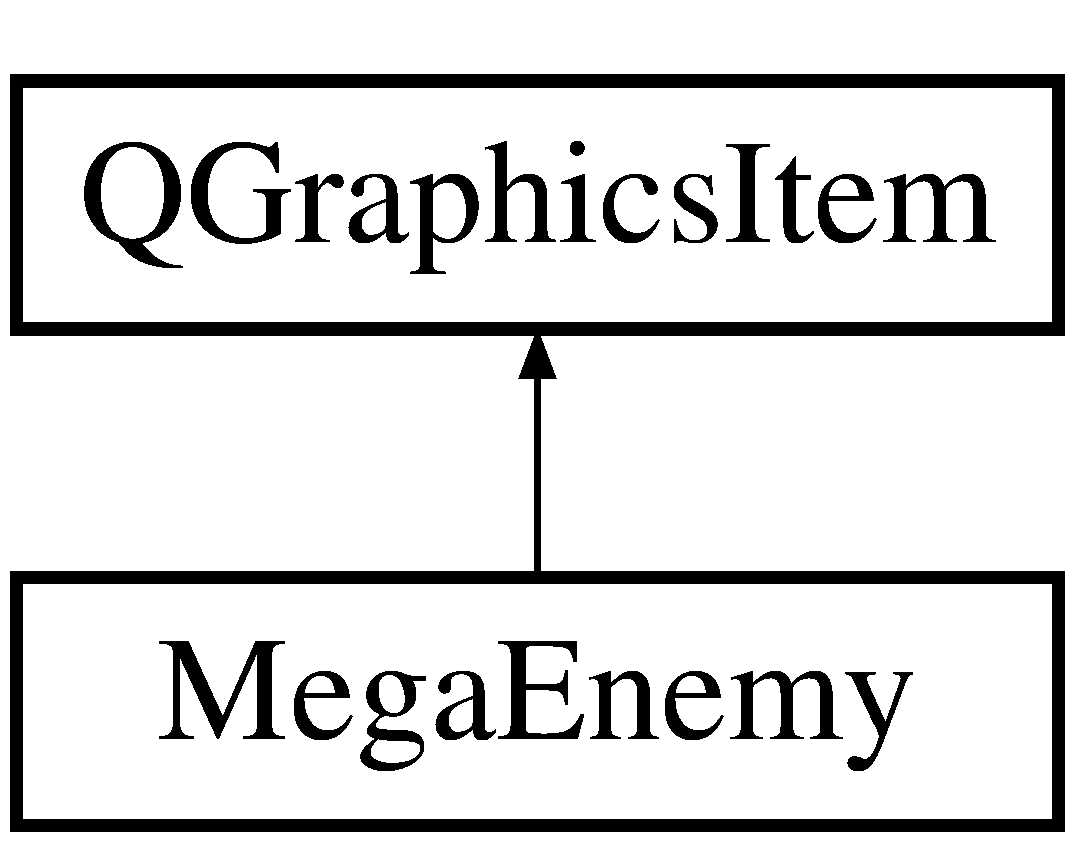
\includegraphics[height=2.000000cm]{class_mega_enemy}
\end{center}
\end{figure}
\subsection*{Public Member Functions}
\begin{DoxyCompactItemize}
\item 
\hyperlink{class_mega_enemy_aa7016a1be5acff2fb9aa38dac872e8ff}{Mega\-Enemy} (Q\-Graphics\-Item $\ast$parent=N\-U\-L\-L)
\begin{DoxyCompactList}\small\item\em \hyperlink{class_mega_enemy_aa7016a1be5acff2fb9aa38dac872e8ff}{Mega\-Enemy\-::\-Mega\-Enemy}. \end{DoxyCompactList}\item 
\hypertarget{class_mega_enemy_a48f76a1191d94ab17876b82c18443016}{\hyperlink{class_mega_enemy_a48f76a1191d94ab17876b82c18443016}{$\sim$\-Mega\-Enemy} ()}\label{class_mega_enemy_a48f76a1191d94ab17876b82c18443016}

\begin{DoxyCompactList}\small\item\em \hyperlink{class_mega_enemy_a48f76a1191d94ab17876b82c18443016}{Mega\-Enemy\-::$\sim$\-Mega\-Enemy}. \end{DoxyCompactList}\end{DoxyCompactItemize}
\subsection*{Protected Member Functions}
\begin{DoxyCompactItemize}
\item 
void \hyperlink{class_mega_enemy_a23192e1d8461ab93f8ea3ec31dfb439f}{paint} (Q\-Painter $\ast$painter, const Q\-Style\-Option\-Graphics\-Item $\ast$option, Q\-Widget $\ast$widget)
\begin{DoxyCompactList}\small\item\em Paints the enemy.. B\-I\-G! \end{DoxyCompactList}\item 
Q\-Rect\-F \hyperlink{class_mega_enemy_aef6f1948a790e170814074502dc84650}{bounding\-Rect} () const 
\begin{DoxyCompactList}\small\item\em the mega enemy's bounding rect. \end{DoxyCompactList}\end{DoxyCompactItemize}


\subsection{Constructor \& Destructor Documentation}
\hypertarget{class_mega_enemy_aa7016a1be5acff2fb9aa38dac872e8ff}{\index{Mega\-Enemy@{Mega\-Enemy}!Mega\-Enemy@{Mega\-Enemy}}
\index{Mega\-Enemy@{Mega\-Enemy}!MegaEnemy@{Mega\-Enemy}}
\subsubsection[{Mega\-Enemy}]{\setlength{\rightskip}{0pt plus 5cm}Mega\-Enemy\-::\-Mega\-Enemy (
\begin{DoxyParamCaption}
\item[{Q\-Graphics\-Item $\ast$}]{parent = {\ttfamily NULL}}
\end{DoxyParamCaption}
)}}\label{class_mega_enemy_aa7016a1be5acff2fb9aa38dac872e8ff}


\hyperlink{class_mega_enemy_aa7016a1be5acff2fb9aa38dac872e8ff}{Mega\-Enemy\-::\-Mega\-Enemy}. 


\begin{DoxyParams}{Parameters}
{\em parent} & \\
\hline
\end{DoxyParams}


\subsection{Member Function Documentation}
\hypertarget{class_mega_enemy_aef6f1948a790e170814074502dc84650}{\index{Mega\-Enemy@{Mega\-Enemy}!bounding\-Rect@{bounding\-Rect}}
\index{bounding\-Rect@{bounding\-Rect}!MegaEnemy@{Mega\-Enemy}}
\subsubsection[{bounding\-Rect}]{\setlength{\rightskip}{0pt plus 5cm}Q\-Rect\-F Mega\-Enemy\-::bounding\-Rect (
\begin{DoxyParamCaption}
{}
\end{DoxyParamCaption}
) const\hspace{0.3cm}{\ttfamily [protected]}}}\label{class_mega_enemy_aef6f1948a790e170814074502dc84650}


the mega enemy's bounding rect. 

\begin{DoxyReturn}{Returns}

\end{DoxyReturn}
\hypertarget{class_mega_enemy_a23192e1d8461ab93f8ea3ec31dfb439f}{\index{Mega\-Enemy@{Mega\-Enemy}!paint@{paint}}
\index{paint@{paint}!MegaEnemy@{Mega\-Enemy}}
\subsubsection[{paint}]{\setlength{\rightskip}{0pt plus 5cm}void Mega\-Enemy\-::paint (
\begin{DoxyParamCaption}
\item[{Q\-Painter $\ast$}]{painter, }
\item[{const Q\-Style\-Option\-Graphics\-Item $\ast$}]{option, }
\item[{Q\-Widget $\ast$}]{widget}
\end{DoxyParamCaption}
)\hspace{0.3cm}{\ttfamily [protected]}}}\label{class_mega_enemy_a23192e1d8461ab93f8ea3ec31dfb439f}


Paints the enemy.. B\-I\-G! 


\begin{DoxyParams}{Parameters}
{\em painter} & \\
\hline
{\em option} & \\
\hline
{\em widget} & \\
\hline
\end{DoxyParams}


The documentation for this class was generated from the following files\-:\begin{DoxyCompactItemize}
\item 
megaenemy.\-h\item 
megaenemy.\-cpp\end{DoxyCompactItemize}

\hypertarget{class_mini_enemy}{\section{Mini\-Enemy Class Reference}
\label{class_mini_enemy}\index{Mini\-Enemy@{Mini\-Enemy}}
}
Inheritance diagram for Mini\-Enemy\-:\begin{figure}[H]
\begin{center}
\leavevmode
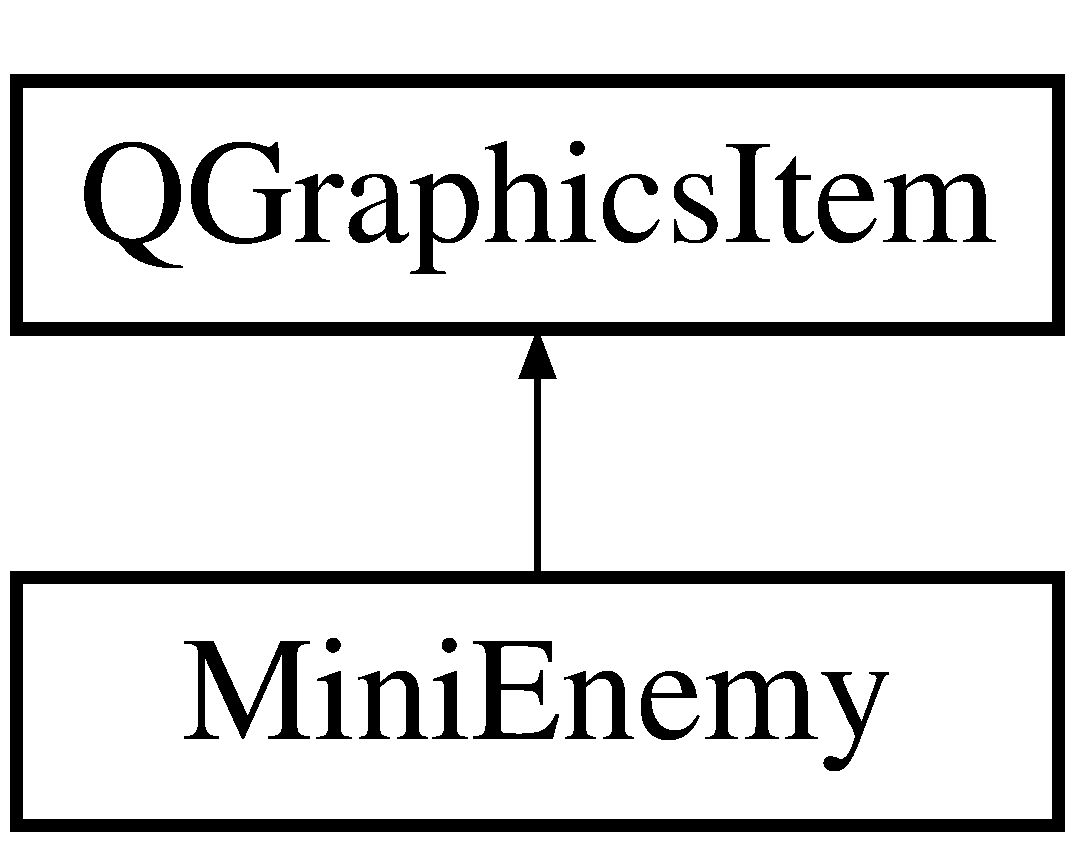
\includegraphics[height=2.000000cm]{class_mini_enemy}
\end{center}
\end{figure}
\subsection*{Public Member Functions}
\begin{DoxyCompactItemize}
\item 
\hyperlink{class_mini_enemy_aa3570678639a19f80f20299c0725600b}{Mini\-Enemy} (Q\-Graphics\-Item $\ast$parent=N\-U\-L\-L)
\begin{DoxyCompactList}\small\item\em \hyperlink{class_mini_enemy_aa3570678639a19f80f20299c0725600b}{Mini\-Enemy\-::\-Mini\-Enemy}. \end{DoxyCompactList}\item 
\hypertarget{class_mini_enemy_a088faaf9cd9af25220621a13ec44cd24}{\hyperlink{class_mini_enemy_a088faaf9cd9af25220621a13ec44cd24}{$\sim$\-Mini\-Enemy} ()}\label{class_mini_enemy_a088faaf9cd9af25220621a13ec44cd24}

\begin{DoxyCompactList}\small\item\em \hyperlink{class_mini_enemy_a088faaf9cd9af25220621a13ec44cd24}{Mini\-Enemy\-::$\sim$\-Mini\-Enemy}. \end{DoxyCompactList}\end{DoxyCompactItemize}
\subsection*{Protected Member Functions}
\begin{DoxyCompactItemize}
\item 
void \hyperlink{class_mini_enemy_afd4f05eaa64c0e666dc59b8967e5cea7}{paint} (Q\-Painter $\ast$painter, const Q\-Style\-Option\-Graphics\-Item $\ast$option, Q\-Widget $\ast$widget)
\begin{DoxyCompactList}\small\item\em Mini\-Enemy\-::paints the enemy. \end{DoxyCompactList}\item 
Q\-Rect\-F \hyperlink{class_mini_enemy_abb6b69c782e02e527610b5e40d56d002}{bounding\-Rect} () const 
\begin{DoxyCompactList}\small\item\em \hyperlink{class_mini_enemy_abb6b69c782e02e527610b5e40d56d002}{Mini\-Enemy\-::bounding\-Rect}. \end{DoxyCompactList}\end{DoxyCompactItemize}


\subsection{Constructor \& Destructor Documentation}
\hypertarget{class_mini_enemy_aa3570678639a19f80f20299c0725600b}{\index{Mini\-Enemy@{Mini\-Enemy}!Mini\-Enemy@{Mini\-Enemy}}
\index{Mini\-Enemy@{Mini\-Enemy}!MiniEnemy@{Mini\-Enemy}}
\subsubsection[{Mini\-Enemy}]{\setlength{\rightskip}{0pt plus 5cm}Mini\-Enemy\-::\-Mini\-Enemy (
\begin{DoxyParamCaption}
\item[{Q\-Graphics\-Item $\ast$}]{parent = {\ttfamily NULL}}
\end{DoxyParamCaption}
)}}\label{class_mini_enemy_aa3570678639a19f80f20299c0725600b}


\hyperlink{class_mini_enemy_aa3570678639a19f80f20299c0725600b}{Mini\-Enemy\-::\-Mini\-Enemy}. 


\begin{DoxyParams}{Parameters}
{\em parent} & \\
\hline
\end{DoxyParams}


\subsection{Member Function Documentation}
\hypertarget{class_mini_enemy_abb6b69c782e02e527610b5e40d56d002}{\index{Mini\-Enemy@{Mini\-Enemy}!bounding\-Rect@{bounding\-Rect}}
\index{bounding\-Rect@{bounding\-Rect}!MiniEnemy@{Mini\-Enemy}}
\subsubsection[{bounding\-Rect}]{\setlength{\rightskip}{0pt plus 5cm}Q\-Rect\-F Mini\-Enemy\-::bounding\-Rect (
\begin{DoxyParamCaption}
{}
\end{DoxyParamCaption}
) const\hspace{0.3cm}{\ttfamily [protected]}}}\label{class_mini_enemy_abb6b69c782e02e527610b5e40d56d002}


\hyperlink{class_mini_enemy_abb6b69c782e02e527610b5e40d56d002}{Mini\-Enemy\-::bounding\-Rect}. 

\begin{DoxyReturn}{Returns}

\end{DoxyReturn}
\hypertarget{class_mini_enemy_afd4f05eaa64c0e666dc59b8967e5cea7}{\index{Mini\-Enemy@{Mini\-Enemy}!paint@{paint}}
\index{paint@{paint}!MiniEnemy@{Mini\-Enemy}}
\subsubsection[{paint}]{\setlength{\rightskip}{0pt plus 5cm}void Mini\-Enemy\-::paint (
\begin{DoxyParamCaption}
\item[{Q\-Painter $\ast$}]{painter, }
\item[{const Q\-Style\-Option\-Graphics\-Item $\ast$}]{option, }
\item[{Q\-Widget $\ast$}]{widget}
\end{DoxyParamCaption}
)\hspace{0.3cm}{\ttfamily [protected]}}}\label{class_mini_enemy_afd4f05eaa64c0e666dc59b8967e5cea7}


Mini\-Enemy\-::paints the enemy. 


\begin{DoxyParams}{Parameters}
{\em painter} & \\
\hline
{\em option} & \\
\hline
{\em widget} & \\
\hline
\end{DoxyParams}


The documentation for this class was generated from the following files\-:\begin{DoxyCompactItemize}
\item 
minienemy.\-h\item 
minienemy.\-cpp\end{DoxyCompactItemize}

\hypertarget{class_ui_1_1_pause}{\section{Ui\-:\-:Pause Class Reference}
\label{class_ui_1_1_pause}\index{Ui\-::\-Pause@{Ui\-::\-Pause}}
}
Inheritance diagram for Ui\-:\-:Pause\-:\begin{figure}[H]
\begin{center}
\leavevmode
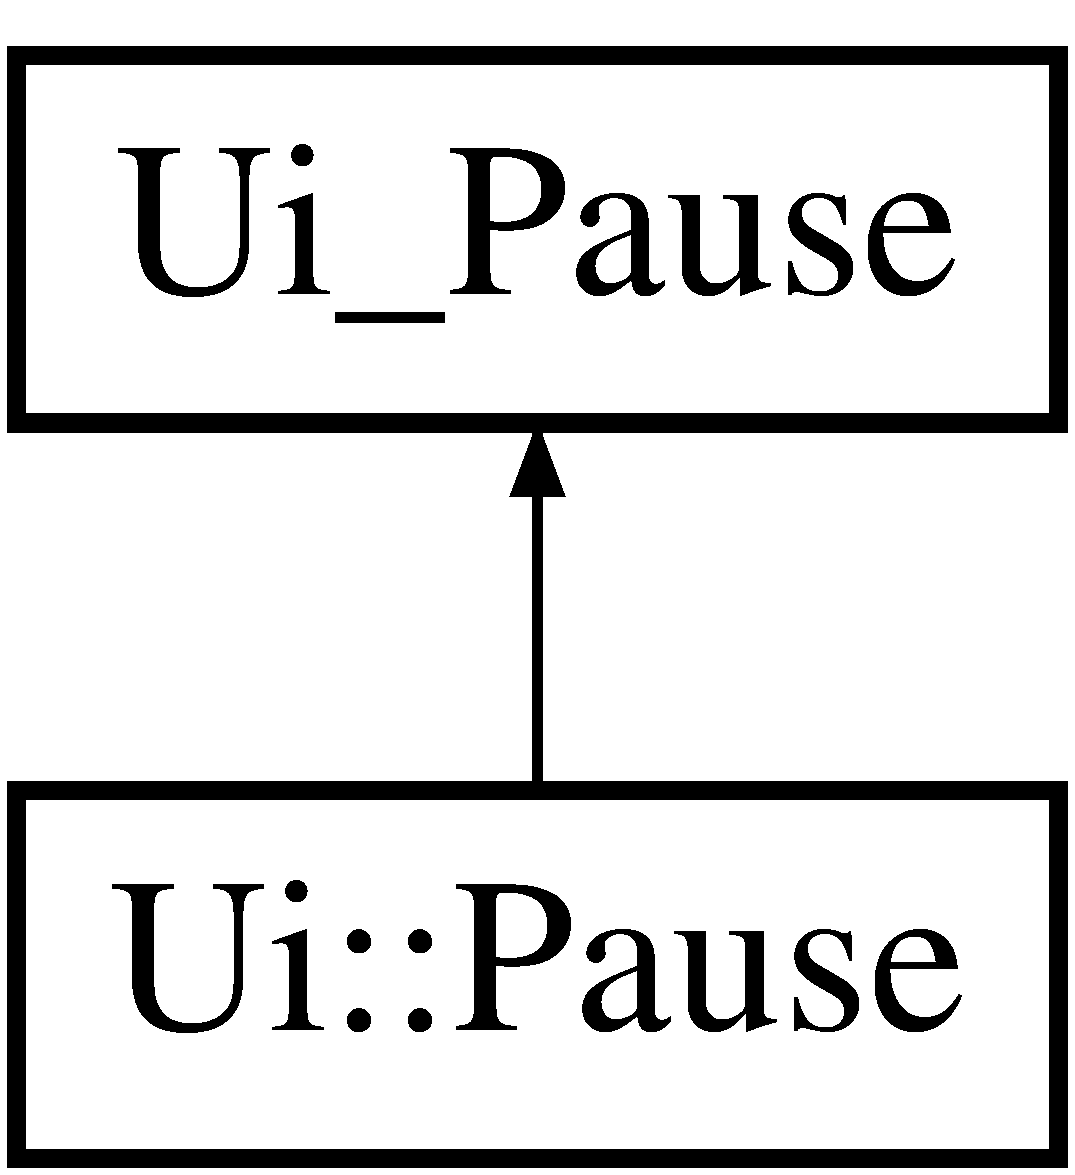
\includegraphics[height=2.000000cm]{class_ui_1_1_pause}
\end{center}
\end{figure}
\subsection*{Additional Inherited Members}


The documentation for this class was generated from the following file\-:\begin{DoxyCompactItemize}
\item 
ui\-\_\-pause.\-h\end{DoxyCompactItemize}

\hypertarget{class_pause}{\section{Pause Class Reference}
\label{class_pause}\index{Pause@{Pause}}
}


This is a \hyperlink{class_pause}{Pause} class. This class will build the pause menu on some key event.  


Inheritance diagram for Pause\-:\begin{figure}[H]
\begin{center}
\leavevmode
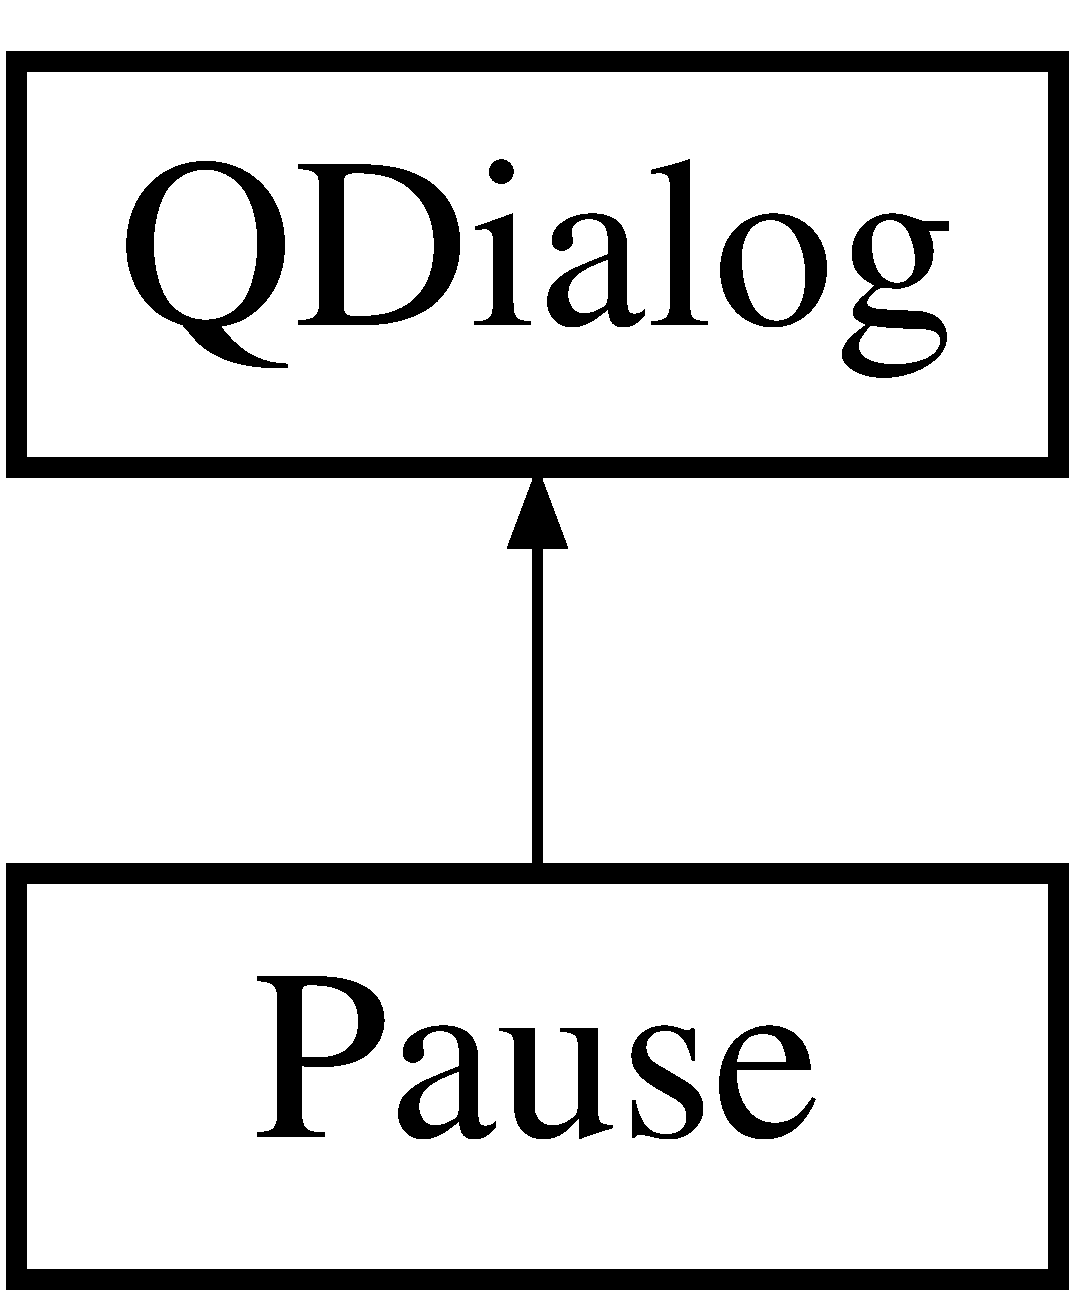
\includegraphics[height=2.000000cm]{class_pause}
\end{center}
\end{figure}
\subsection*{Public Slots}
\begin{DoxyCompactItemize}
\item 
void \hyperlink{class_pause_ad632066c1f745b88f328f609de26419f}{on\-\_\-resume\-\_\-clicked} ()
\begin{DoxyCompactList}\small\item\em on\-\_\-resume\-\_\-clicked Resume game \end{DoxyCompactList}\item 
void \hyperlink{class_pause_aed0cb80fa11b7556ffe285bb83696e55}{on\-\_\-exit\-\_\-clicked} ()
\begin{DoxyCompactList}\small\item\em on\-\_\-exit\-\_\-clicked Exits game \end{DoxyCompactList}\item 
\hypertarget{class_pause_a2b4c1e4ee50785bcca1dc1c422f527b3}{void \hyperlink{class_pause_a2b4c1e4ee50785bcca1dc1c422f527b3}{on\-\_\-progress\-Bar\-\_\-value\-Changed} (int value)}\label{class_pause_a2b4c1e4ee50785bcca1dc1c422f527b3}

\begin{DoxyCompactList}\small\item\em on\-\_\-progress\-Bar\-\_\-value\-Changed monitors health status \end{DoxyCompactList}\end{DoxyCompactItemize}
\subsection*{Public Member Functions}
\begin{DoxyCompactItemize}
\item 
\hyperlink{class_pause_a2677e62030e9d138bc9994f9d6bd727b}{Pause} (Q\-Widget $\ast$parent=0)
\begin{DoxyCompactList}\small\item\em \hyperlink{class_pause}{Pause} constructor will create \hyperlink{class_pause}{Pause} Ui. \end{DoxyCompactList}\item 
\hypertarget{class_pause_a6a564235e87326133c14069be196eeac}{\hyperlink{class_pause_a6a564235e87326133c14069be196eeac}{$\sim$\-Pause} ()}\label{class_pause_a6a564235e87326133c14069be196eeac}

\begin{DoxyCompactList}\small\item\em \hyperlink{class_pause_a6a564235e87326133c14069be196eeac}{Pause\-::$\sim$\-Pause} \hyperlink{class_pause}{Pause} destructor. \end{DoxyCompactList}\end{DoxyCompactItemize}


\subsection{Detailed Description}
This is a \hyperlink{class_pause}{Pause} class. This class will build the pause menu on some key event. 

\subsection{Constructor \& Destructor Documentation}
\hypertarget{class_pause_a2677e62030e9d138bc9994f9d6bd727b}{\index{Pause@{Pause}!Pause@{Pause}}
\index{Pause@{Pause}!Pause@{Pause}}
\subsubsection[{Pause}]{\setlength{\rightskip}{0pt plus 5cm}Pause\-::\-Pause (
\begin{DoxyParamCaption}
\item[{Q\-Widget $\ast$}]{parent = {\ttfamily 0}}
\end{DoxyParamCaption}
)\hspace{0.3cm}{\ttfamily [explicit]}}}\label{class_pause_a2677e62030e9d138bc9994f9d6bd727b}


\hyperlink{class_pause}{Pause} constructor will create \hyperlink{class_pause}{Pause} Ui. 

\hyperlink{class_pause_a2677e62030e9d138bc9994f9d6bd727b}{Pause\-::\-Pause} constructor to build \hyperlink{class_pause}{Pause} menu.


\begin{DoxyParams}{Parameters}
{\em parent} & is passed to \hyperlink{class_pause}{Pause} Ui\\
\hline
{\em parent} & pointer from main window \\
\hline
\end{DoxyParams}


\subsection{Member Function Documentation}
\hypertarget{class_pause_aed0cb80fa11b7556ffe285bb83696e55}{\index{Pause@{Pause}!on\-\_\-exit\-\_\-clicked@{on\-\_\-exit\-\_\-clicked}}
\index{on\-\_\-exit\-\_\-clicked@{on\-\_\-exit\-\_\-clicked}!Pause@{Pause}}
\subsubsection[{on\-\_\-exit\-\_\-clicked}]{\setlength{\rightskip}{0pt plus 5cm}void Pause\-::on\-\_\-exit\-\_\-clicked (
\begin{DoxyParamCaption}
{}
\end{DoxyParamCaption}
)\hspace{0.3cm}{\ttfamily [slot]}}}\label{class_pause_aed0cb80fa11b7556ffe285bb83696e55}


on\-\_\-exit\-\_\-clicked Exits game 

\hyperlink{class_pause_aed0cb80fa11b7556ffe285bb83696e55}{Pause\-::on\-\_\-exit\-\_\-clicked} exit game. \hypertarget{class_pause_ad632066c1f745b88f328f609de26419f}{\index{Pause@{Pause}!on\-\_\-resume\-\_\-clicked@{on\-\_\-resume\-\_\-clicked}}
\index{on\-\_\-resume\-\_\-clicked@{on\-\_\-resume\-\_\-clicked}!Pause@{Pause}}
\subsubsection[{on\-\_\-resume\-\_\-clicked}]{\setlength{\rightskip}{0pt plus 5cm}void Pause\-::on\-\_\-resume\-\_\-clicked (
\begin{DoxyParamCaption}
{}
\end{DoxyParamCaption}
)\hspace{0.3cm}{\ttfamily [slot]}}}\label{class_pause_ad632066c1f745b88f328f609de26419f}


on\-\_\-resume\-\_\-clicked Resume game 

\hyperlink{class_pause_ad632066c1f745b88f328f609de26419f}{Pause\-::on\-\_\-resume\-\_\-clicked} resume game. 

The documentation for this class was generated from the following files\-:\begin{DoxyCompactItemize}
\item 
pause.\-h\item 
pause.\-cpp\end{DoxyCompactItemize}

\hypertarget{structqt__meta__stringdata___battle_pause__t}{\section{qt\-\_\-meta\-\_\-stringdata\-\_\-\-Battle\-Pause\-\_\-t Struct Reference}
\label{structqt__meta__stringdata___battle_pause__t}\index{qt\-\_\-meta\-\_\-stringdata\-\_\-\-Battle\-Pause\-\_\-t@{qt\-\_\-meta\-\_\-stringdata\-\_\-\-Battle\-Pause\-\_\-t}}
}
\subsection*{Public Attributes}
\begin{DoxyCompactItemize}
\item 
\hypertarget{structqt__meta__stringdata___battle_pause__t_aca48ea4e086c761c58a0ff64de16ebef}{Q\-Byte\-Array\-Data {\bfseries data} \mbox{[}3\mbox{]}}\label{structqt__meta__stringdata___battle_pause__t_aca48ea4e086c761c58a0ff64de16ebef}

\item 
\hypertarget{structqt__meta__stringdata___battle_pause__t_a9db2cc35cd32f230a8536f6394012e16}{char {\bfseries stringdata} \mbox{[}36\mbox{]}}\label{structqt__meta__stringdata___battle_pause__t_a9db2cc35cd32f230a8536f6394012e16}

\end{DoxyCompactItemize}


The documentation for this struct was generated from the following file\-:\begin{DoxyCompactItemize}
\item 
moc\-\_\-battlepause.\-cpp\end{DoxyCompactItemize}

\hypertarget{structqt__meta__stringdata___main_window__t}{\section{qt\-\_\-meta\-\_\-stringdata\-\_\-\-Main\-Window\-\_\-t Struct Reference}
\label{structqt__meta__stringdata___main_window__t}\index{qt\-\_\-meta\-\_\-stringdata\-\_\-\-Main\-Window\-\_\-t@{qt\-\_\-meta\-\_\-stringdata\-\_\-\-Main\-Window\-\_\-t}}
}
\subsection*{Public Attributes}
\begin{DoxyCompactItemize}
\item 
\hypertarget{structqt__meta__stringdata___main_window__t_a332d7fa058028f7613b5ba68abb5a7fe}{Q\-Byte\-Array\-Data {\bfseries data} \mbox{[}4\mbox{]}}\label{structqt__meta__stringdata___main_window__t_a332d7fa058028f7613b5ba68abb5a7fe}

\item 
\hypertarget{structqt__meta__stringdata___main_window__t_a1f75f6e6169dcfddb4a6e5701e72456e}{char {\bfseries stringdata} \mbox{[}59\mbox{]}}\label{structqt__meta__stringdata___main_window__t_a1f75f6e6169dcfddb4a6e5701e72456e}

\end{DoxyCompactItemize}


The documentation for this struct was generated from the following file\-:\begin{DoxyCompactItemize}
\item 
moc\-\_\-mainwindow.\-cpp\end{DoxyCompactItemize}

\hypertarget{structqt__meta__stringdata___pause__t}{\section{qt\-\_\-meta\-\_\-stringdata\-\_\-\-Pause\-\_\-t Struct Reference}
\label{structqt__meta__stringdata___pause__t}\index{qt\-\_\-meta\-\_\-stringdata\-\_\-\-Pause\-\_\-t@{qt\-\_\-meta\-\_\-stringdata\-\_\-\-Pause\-\_\-t}}
}
\subsection*{Public Attributes}
\begin{DoxyCompactItemize}
\item 
\hypertarget{structqt__meta__stringdata___pause__t_a0db72ef1c0f4f2b70a413bfb498ba07e}{Q\-Byte\-Array\-Data {\bfseries data} \mbox{[}4\mbox{]}}\label{structqt__meta__stringdata___pause__t_a0db72ef1c0f4f2b70a413bfb498ba07e}

\item 
\hypertarget{structqt__meta__stringdata___pause__t_ad4433c46256c70c2634dcf0c941a2476}{char {\bfseries stringdata} \mbox{[}42\mbox{]}}\label{structqt__meta__stringdata___pause__t_ad4433c46256c70c2634dcf0c941a2476}

\end{DoxyCompactItemize}


The documentation for this struct was generated from the following file\-:\begin{DoxyCompactItemize}
\item 
moc\-\_\-pause.\-cpp\end{DoxyCompactItemize}

\hypertarget{structqt__meta__stringdata__worldmap__t}{\section{qt\-\_\-meta\-\_\-stringdata\-\_\-worldmap\-\_\-t Struct Reference}
\label{structqt__meta__stringdata__worldmap__t}\index{qt\-\_\-meta\-\_\-stringdata\-\_\-worldmap\-\_\-t@{qt\-\_\-meta\-\_\-stringdata\-\_\-worldmap\-\_\-t}}
}
\subsection*{Public Attributes}
\begin{DoxyCompactItemize}
\item 
\hypertarget{structqt__meta__stringdata__worldmap__t_a7f053666ef1690a4a6f61446cfade706}{Q\-Byte\-Array\-Data {\bfseries data} \mbox{[}3\mbox{]}}\label{structqt__meta__stringdata__worldmap__t_a7f053666ef1690a4a6f61446cfade706}

\item 
\hypertarget{structqt__meta__stringdata__worldmap__t_a1d1ac6d61c17f43deb7020712a1c3eca}{char {\bfseries stringdata} \mbox{[}33\mbox{]}}\label{structqt__meta__stringdata__worldmap__t_a1d1ac6d61c17f43deb7020712a1c3eca}

\end{DoxyCompactItemize}


The documentation for this struct was generated from the following file\-:\begin{DoxyCompactItemize}
\item 
moc\-\_\-worldmap.\-cpp\end{DoxyCompactItemize}

\hypertarget{classshotgun}{\section{shotgun Class Reference}
\label{classshotgun}\index{shotgun@{shotgun}}
}
Inheritance diagram for shotgun\-:\begin{figure}[H]
\begin{center}
\leavevmode
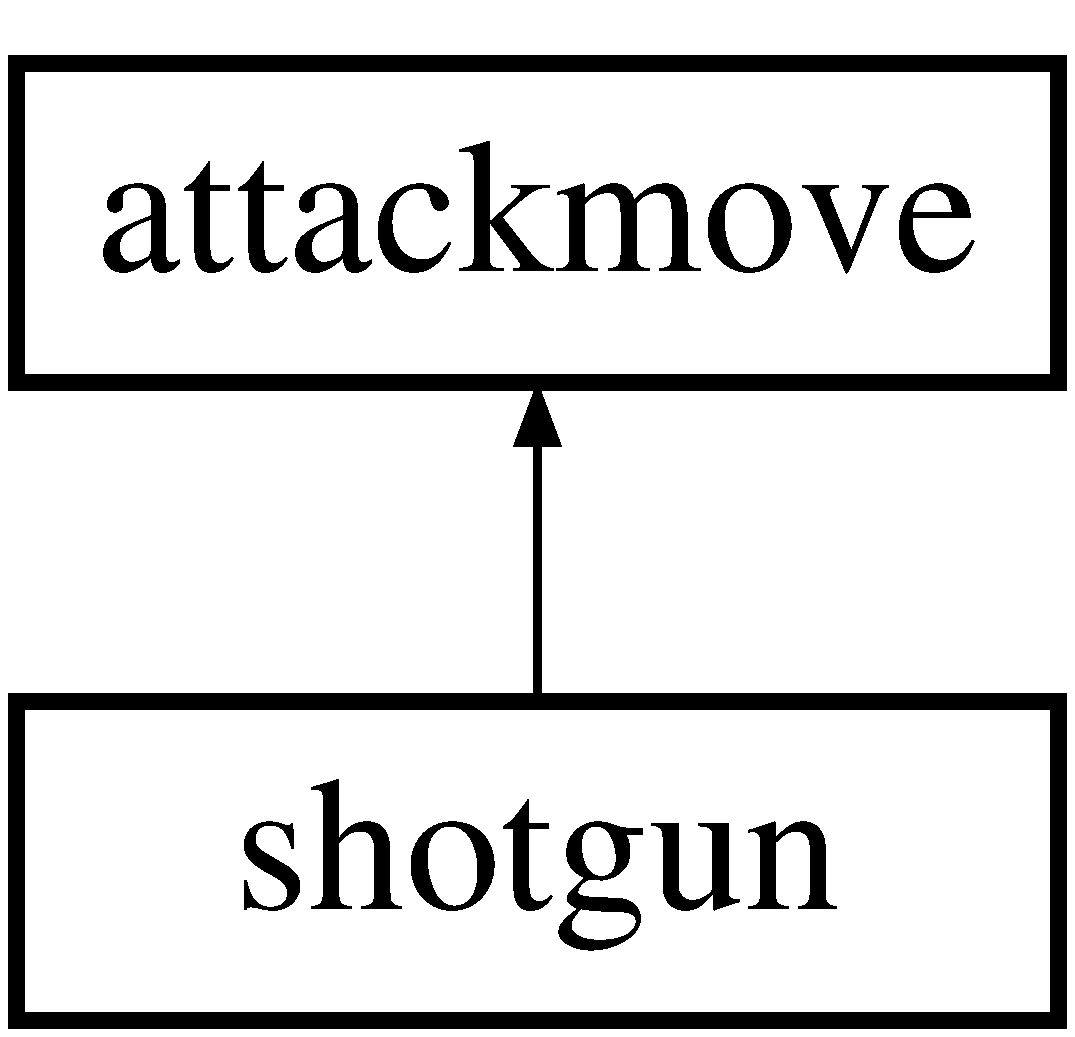
\includegraphics[height=2.000000cm]{classshotgun}
\end{center}
\end{figure}
\subsection*{Public Member Functions}
\begin{DoxyCompactItemize}
\item 
\hypertarget{classshotgun_adbc12267b0204869263cd2813fb6ccc1}{{\bfseries shotgun} (int dam)}\label{classshotgun_adbc12267b0204869263cd2813fb6ccc1}

\item 
virtual Q\-String \hyperlink{classshotgun_a856fa8335ee3c2bb8603e83aa5629e5c}{get\-String} ()
\begin{DoxyCompactList}\small\item\em \hyperlink{classattackmove_ada49eedf4b893372c576edd48fe73161}{attackmove\-::get\-String} \end{DoxyCompactList}\item 
virtual Q\-Image \hyperlink{classshotgun_a1336af80f8d3f7d19ac954f2e616a1b0}{get\-Image} ()
\begin{DoxyCompactList}\small\item\em \hyperlink{classattackmove_aca59a2343b7a6c195d300dda5c8d952d}{attackmove\-::get\-Image} \end{DoxyCompactList}\item 
virtual void \hyperlink{classshotgun_a8334202fd30d71432db7e58fca7a462e}{get\-Hover} (int hpanel, \hyperlink{class_enemy}{Enemy} $\ast$Enemies\mbox{[}3\mbox{]}, \hyperlink{classanim_items}{anim\-Items} $\ast$anim)
\begin{DoxyCompactList}\small\item\em \hyperlink{classattackmove_a0ff82349551bd72f4d57b3367bb318fa}{attackmove\-::get\-Hover} \end{DoxyCompactList}\item 
\hypertarget{classshotgun_a38d2c751cb6f3bed896d8d71c5354de5}{virtual void {\bfseries do\-Attack} (int hpanel, \hyperlink{class_enemy}{Enemy} $\ast$Enemies\mbox{[}$\,$\mbox{]}, \hyperlink{classanim_items}{anim\-Items} $\ast$anim)}\label{classshotgun_a38d2c751cb6f3bed896d8d71c5354de5}

\end{DoxyCompactItemize}
\subsection*{Additional Inherited Members}


\subsection{Member Function Documentation}
\hypertarget{classshotgun_a8334202fd30d71432db7e58fca7a462e}{\index{shotgun@{shotgun}!get\-Hover@{get\-Hover}}
\index{get\-Hover@{get\-Hover}!shotgun@{shotgun}}
\subsubsection[{get\-Hover}]{\setlength{\rightskip}{0pt plus 5cm}void shotgun\-::get\-Hover (
\begin{DoxyParamCaption}
\item[{int}]{hpanel, }
\item[{{\bf Enemy} $\ast$}]{Enemies\mbox{[}3\mbox{]}, }
\item[{{\bf anim\-Items} $\ast$}]{anim}
\end{DoxyParamCaption}
)\hspace{0.3cm}{\ttfamily [virtual]}}}\label{classshotgun_a8334202fd30d71432db7e58fca7a462e}


\hyperlink{classattackmove_a0ff82349551bd72f4d57b3367bb318fa}{attackmove\-::get\-Hover} 


\begin{DoxyParams}{Parameters}
{\em hpanel} & \\
\hline
{\em Enemies} & \\
\hline
{\em anim} & \\
\hline
\end{DoxyParams}


Reimplemented from \hyperlink{classattackmove_a0ff82349551bd72f4d57b3367bb318fa}{attackmove}.

\hypertarget{classshotgun_a1336af80f8d3f7d19ac954f2e616a1b0}{\index{shotgun@{shotgun}!get\-Image@{get\-Image}}
\index{get\-Image@{get\-Image}!shotgun@{shotgun}}
\subsubsection[{get\-Image}]{\setlength{\rightskip}{0pt plus 5cm}Q\-Image shotgun\-::get\-Image (
\begin{DoxyParamCaption}
{}
\end{DoxyParamCaption}
)\hspace{0.3cm}{\ttfamily [virtual]}}}\label{classshotgun_a1336af80f8d3f7d19ac954f2e616a1b0}


\hyperlink{classattackmove_aca59a2343b7a6c195d300dda5c8d952d}{attackmove\-::get\-Image} 

\begin{DoxyReturn}{Returns}

\end{DoxyReturn}


Reimplemented from \hyperlink{classattackmove_aca59a2343b7a6c195d300dda5c8d952d}{attackmove}.

\hypertarget{classshotgun_a856fa8335ee3c2bb8603e83aa5629e5c}{\index{shotgun@{shotgun}!get\-String@{get\-String}}
\index{get\-String@{get\-String}!shotgun@{shotgun}}
\subsubsection[{get\-String}]{\setlength{\rightskip}{0pt plus 5cm}Q\-String shotgun\-::get\-String (
\begin{DoxyParamCaption}
{}
\end{DoxyParamCaption}
)\hspace{0.3cm}{\ttfamily [virtual]}}}\label{classshotgun_a856fa8335ee3c2bb8603e83aa5629e5c}


\hyperlink{classattackmove_ada49eedf4b893372c576edd48fe73161}{attackmove\-::get\-String} 

\begin{DoxyReturn}{Returns}
string of name, implemented in all inheritences includes damage 
\end{DoxyReturn}


Reimplemented from \hyperlink{classattackmove_ada49eedf4b893372c576edd48fe73161}{attackmove}.



The documentation for this class was generated from the following files\-:\begin{DoxyCompactItemize}
\item 
shotgun.\-h\item 
shotgun.\-cpp\end{DoxyCompactItemize}

\hypertarget{class_skeleton}{\section{Skeleton Class Reference}
\label{class_skeleton}\index{Skeleton@{Skeleton}}
}
Inheritance diagram for Skeleton\-:\begin{figure}[H]
\begin{center}
\leavevmode
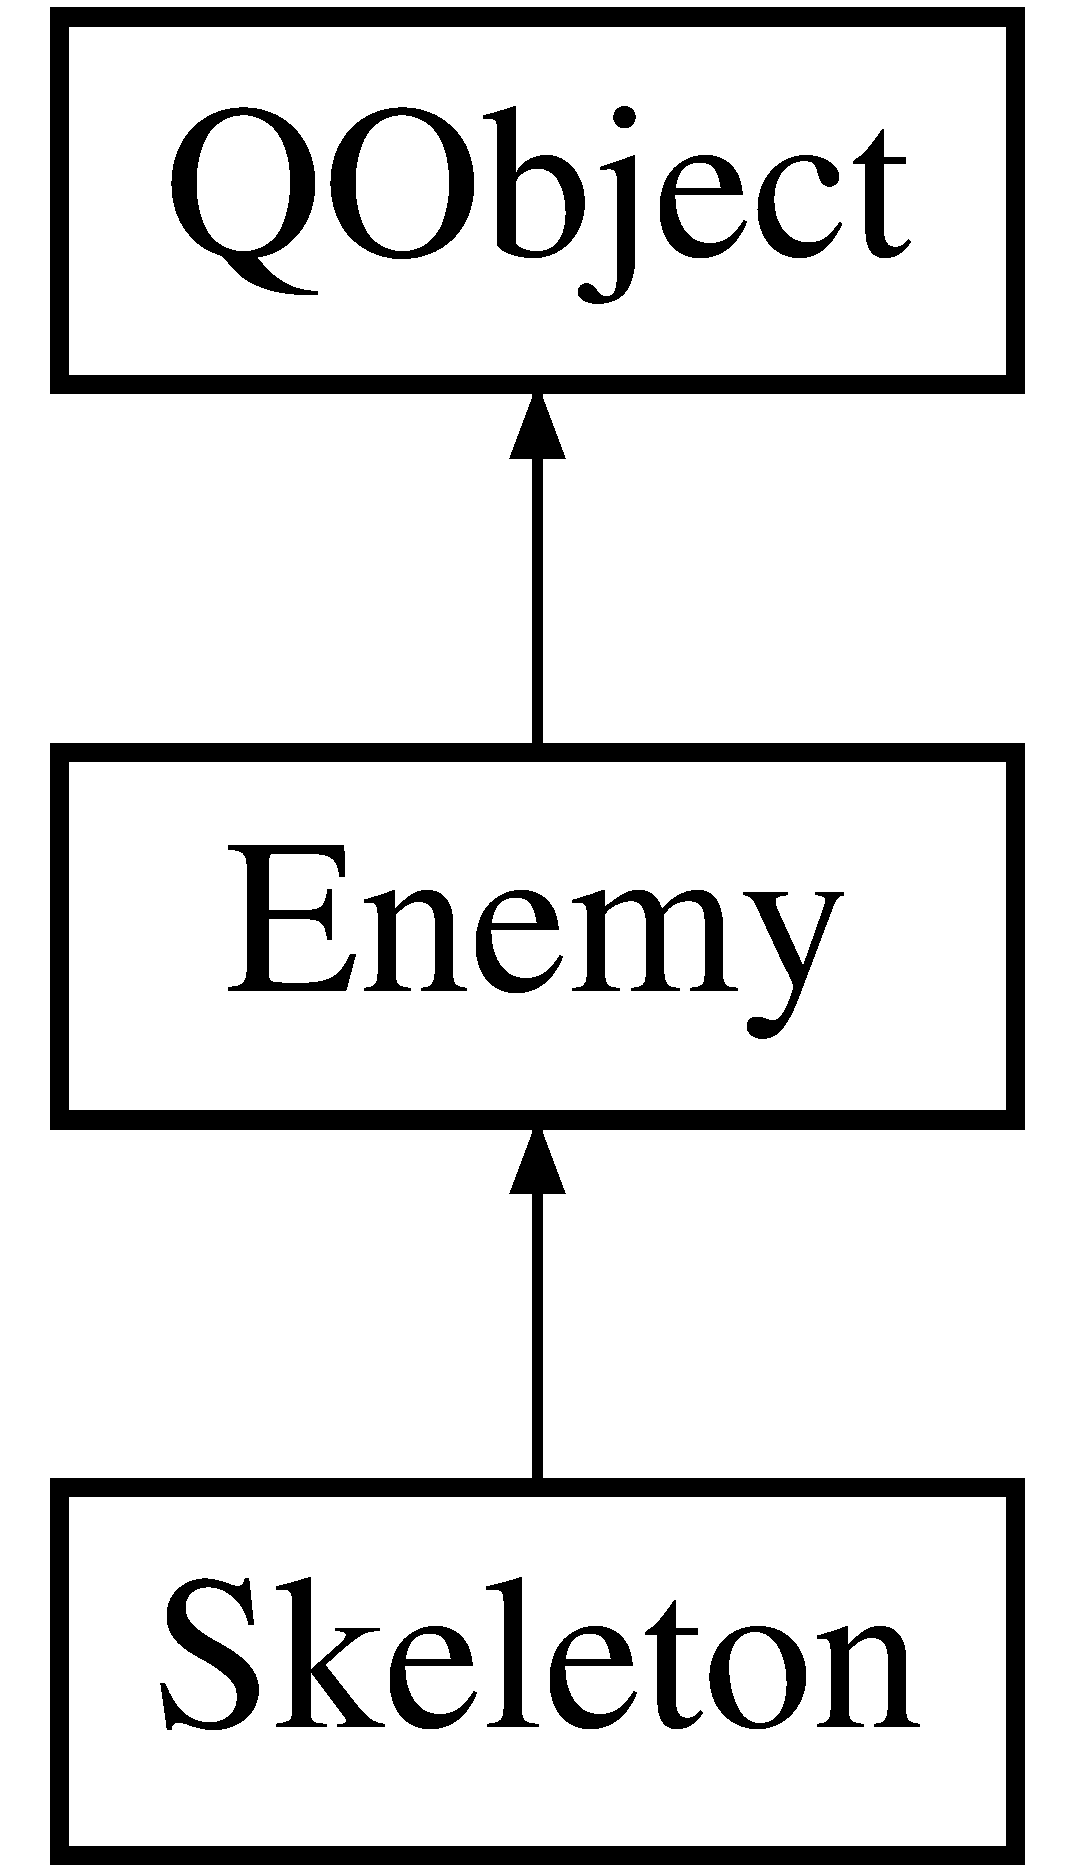
\includegraphics[height=3.000000cm]{class_skeleton}
\end{center}
\end{figure}
\subsection*{Public Member Functions}
\begin{DoxyCompactItemize}
\item 
\hypertarget{class_skeleton_ac4920b7ab446add4c8da5c8fe6aff2d3}{{\bfseries Skeleton} (int clev, int cx, int cy)}\label{class_skeleton_ac4920b7ab446add4c8da5c8fe6aff2d3}

\item 
virtual void \hyperlink{class_skeleton_aeb5642a3aa8c49cb0cd1cc325f8f0baa}{do\-Turn} (\hyperlink{class_character}{Character} $\ast$Hero)
\begin{DoxyCompactList}\small\item\em \hyperlink{class_enemy_a56e4b9b07e8cd2a4e5ecfa8ff5b9265a}{Enemy\-::do\-Turn} based on hero's panel, does it's move. \end{DoxyCompactList}\item 
\hypertarget{class_skeleton_a35acfe2e2da4279a56d91bb8f2048489}{virtual Q\-Image {\bfseries get\-Pic} ()}\label{class_skeleton_a35acfe2e2da4279a56d91bb8f2048489}

\item 
virtual void \hyperlink{class_skeleton_ae605f24f6e921ad3b36a53f391304722}{draw\-Self} (Q\-Painter $\ast$g, int gx, int gy)
\begin{DoxyCompactList}\small\item\em \hyperlink{class_enemy_a3251244e8e7ac657687d6be5a8da71bb}{Enemy\-::draw\-Self} draws itself using painter, includes title and hp. \end{DoxyCompactList}\end{DoxyCompactItemize}
\subsection*{Additional Inherited Members}


\subsection{Member Function Documentation}
\hypertarget{class_skeleton_aeb5642a3aa8c49cb0cd1cc325f8f0baa}{\index{Skeleton@{Skeleton}!do\-Turn@{do\-Turn}}
\index{do\-Turn@{do\-Turn}!Skeleton@{Skeleton}}
\subsubsection[{do\-Turn}]{\setlength{\rightskip}{0pt plus 5cm}void Skeleton\-::do\-Turn (
\begin{DoxyParamCaption}
\item[{{\bf Character} $\ast$}]{Hero}
\end{DoxyParamCaption}
)\hspace{0.3cm}{\ttfamily [virtual]}}}\label{class_skeleton_aeb5642a3aa8c49cb0cd1cc325f8f0baa}


\hyperlink{class_enemy_a56e4b9b07e8cd2a4e5ecfa8ff5b9265a}{Enemy\-::do\-Turn} based on hero's panel, does it's move. 


\begin{DoxyParams}{Parameters}
{\em Hero} & \\
\hline
\end{DoxyParams}


Reimplemented from \hyperlink{class_enemy_a56e4b9b07e8cd2a4e5ecfa8ff5b9265a}{Enemy}.

\hypertarget{class_skeleton_ae605f24f6e921ad3b36a53f391304722}{\index{Skeleton@{Skeleton}!draw\-Self@{draw\-Self}}
\index{draw\-Self@{draw\-Self}!Skeleton@{Skeleton}}
\subsubsection[{draw\-Self}]{\setlength{\rightskip}{0pt plus 5cm}void Skeleton\-::draw\-Self (
\begin{DoxyParamCaption}
\item[{Q\-Painter $\ast$}]{g, }
\item[{int}]{gx, }
\item[{int}]{gy}
\end{DoxyParamCaption}
)\hspace{0.3cm}{\ttfamily [virtual]}}}\label{class_skeleton_ae605f24f6e921ad3b36a53f391304722}


\hyperlink{class_enemy_a3251244e8e7ac657687d6be5a8da71bb}{Enemy\-::draw\-Self} draws itself using painter, includes title and hp. 


\begin{DoxyParams}{Parameters}
{\em g} & \\
\hline
{\em gx} & \\
\hline
{\em gy} & \\
\hline
\end{DoxyParams}


Reimplemented from \hyperlink{class_enemy_a3251244e8e7ac657687d6be5a8da71bb}{Enemy}.



The documentation for this class was generated from the following files\-:\begin{DoxyCompactItemize}
\item 
skeleton.\-h\item 
skeleton.\-cpp\end{DoxyCompactItemize}

\hypertarget{classswordslash}{\section{swordslash Class Reference}
\label{classswordslash}\index{swordslash@{swordslash}}
}
Inheritance diagram for swordslash\-:\begin{figure}[H]
\begin{center}
\leavevmode
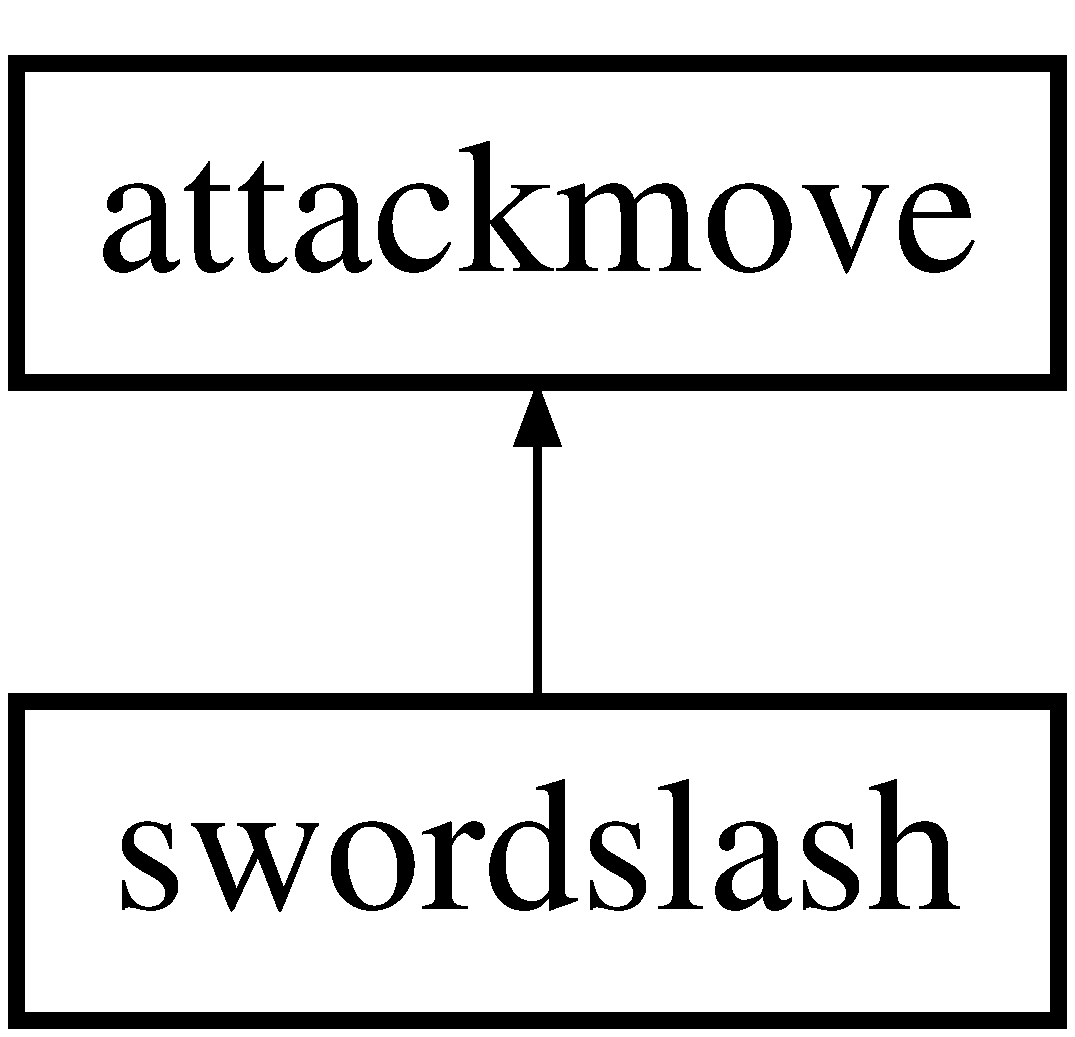
\includegraphics[height=2.000000cm]{classswordslash}
\end{center}
\end{figure}
\subsection*{Public Member Functions}
\begin{DoxyCompactItemize}
\item 
\hypertarget{classswordslash_a1c4547e783632e2e3e42642754dfb6ea}{{\bfseries swordslash} (int dam)}\label{classswordslash_a1c4547e783632e2e3e42642754dfb6ea}

\item 
virtual Q\-String \hyperlink{classswordslash_ac58a7e3b969bb957548c55bdfd6a0b05}{get\-String} ()
\begin{DoxyCompactList}\small\item\em \hyperlink{classattackmove_ada49eedf4b893372c576edd48fe73161}{attackmove\-::get\-String} \end{DoxyCompactList}\item 
virtual Q\-Image \hyperlink{classswordslash_a25cbfa2df6b5718a299eed09cf716822}{get\-Image} ()
\begin{DoxyCompactList}\small\item\em \hyperlink{classattackmove_aca59a2343b7a6c195d300dda5c8d952d}{attackmove\-::get\-Image} \end{DoxyCompactList}\item 
virtual void \hyperlink{classswordslash_af40c617c0463f788bda02fe5e8109511}{get\-Hover} (int hpanel, \hyperlink{class_enemy}{Enemy} $\ast$Enemies\mbox{[}3\mbox{]}, \hyperlink{classanim_items}{anim\-Items} $\ast$anim)
\begin{DoxyCompactList}\small\item\em \hyperlink{classattackmove_a0ff82349551bd72f4d57b3367bb318fa}{attackmove\-::get\-Hover} \end{DoxyCompactList}\item 
\hypertarget{classswordslash_a8583edccf2f8b5635797e6891f797211}{virtual void {\bfseries do\-Attack} (int hpanel, \hyperlink{class_enemy}{Enemy} $\ast$Enemies\mbox{[}$\,$\mbox{]}, \hyperlink{classanim_items}{anim\-Items} $\ast$anim)}\label{classswordslash_a8583edccf2f8b5635797e6891f797211}

\end{DoxyCompactItemize}
\subsection*{Additional Inherited Members}


\subsection{Member Function Documentation}
\hypertarget{classswordslash_af40c617c0463f788bda02fe5e8109511}{\index{swordslash@{swordslash}!get\-Hover@{get\-Hover}}
\index{get\-Hover@{get\-Hover}!swordslash@{swordslash}}
\subsubsection[{get\-Hover}]{\setlength{\rightskip}{0pt plus 5cm}void swordslash\-::get\-Hover (
\begin{DoxyParamCaption}
\item[{int}]{hpanel, }
\item[{{\bf Enemy} $\ast$}]{Enemies\mbox{[}3\mbox{]}, }
\item[{{\bf anim\-Items} $\ast$}]{anim}
\end{DoxyParamCaption}
)\hspace{0.3cm}{\ttfamily [virtual]}}}\label{classswordslash_af40c617c0463f788bda02fe5e8109511}


\hyperlink{classattackmove_a0ff82349551bd72f4d57b3367bb318fa}{attackmove\-::get\-Hover} 


\begin{DoxyParams}{Parameters}
{\em hpanel} & \\
\hline
{\em Enemies} & \\
\hline
{\em anim} & \\
\hline
\end{DoxyParams}


Reimplemented from \hyperlink{classattackmove_a0ff82349551bd72f4d57b3367bb318fa}{attackmove}.

\hypertarget{classswordslash_a25cbfa2df6b5718a299eed09cf716822}{\index{swordslash@{swordslash}!get\-Image@{get\-Image}}
\index{get\-Image@{get\-Image}!swordslash@{swordslash}}
\subsubsection[{get\-Image}]{\setlength{\rightskip}{0pt plus 5cm}Q\-Image swordslash\-::get\-Image (
\begin{DoxyParamCaption}
{}
\end{DoxyParamCaption}
)\hspace{0.3cm}{\ttfamily [virtual]}}}\label{classswordslash_a25cbfa2df6b5718a299eed09cf716822}


\hyperlink{classattackmove_aca59a2343b7a6c195d300dda5c8d952d}{attackmove\-::get\-Image} 

\begin{DoxyReturn}{Returns}

\end{DoxyReturn}


Reimplemented from \hyperlink{classattackmove_aca59a2343b7a6c195d300dda5c8d952d}{attackmove}.

\hypertarget{classswordslash_ac58a7e3b969bb957548c55bdfd6a0b05}{\index{swordslash@{swordslash}!get\-String@{get\-String}}
\index{get\-String@{get\-String}!swordslash@{swordslash}}
\subsubsection[{get\-String}]{\setlength{\rightskip}{0pt plus 5cm}Q\-String swordslash\-::get\-String (
\begin{DoxyParamCaption}
{}
\end{DoxyParamCaption}
)\hspace{0.3cm}{\ttfamily [virtual]}}}\label{classswordslash_ac58a7e3b969bb957548c55bdfd6a0b05}


\hyperlink{classattackmove_ada49eedf4b893372c576edd48fe73161}{attackmove\-::get\-String} 

\begin{DoxyReturn}{Returns}
string of name, implemented in all inheritences includes damage 
\end{DoxyReturn}


Reimplemented from \hyperlink{classattackmove_ada49eedf4b893372c576edd48fe73161}{attackmove}.



The documentation for this class was generated from the following files\-:\begin{DoxyCompactItemize}
\item 
swordslash.\-h\item 
swordslash.\-cpp\end{DoxyCompactItemize}

\hypertarget{classswordsman}{\section{swordsman Class Reference}
\label{classswordsman}\index{swordsman@{swordsman}}
}
Inheritance diagram for swordsman\-:\begin{figure}[H]
\begin{center}
\leavevmode
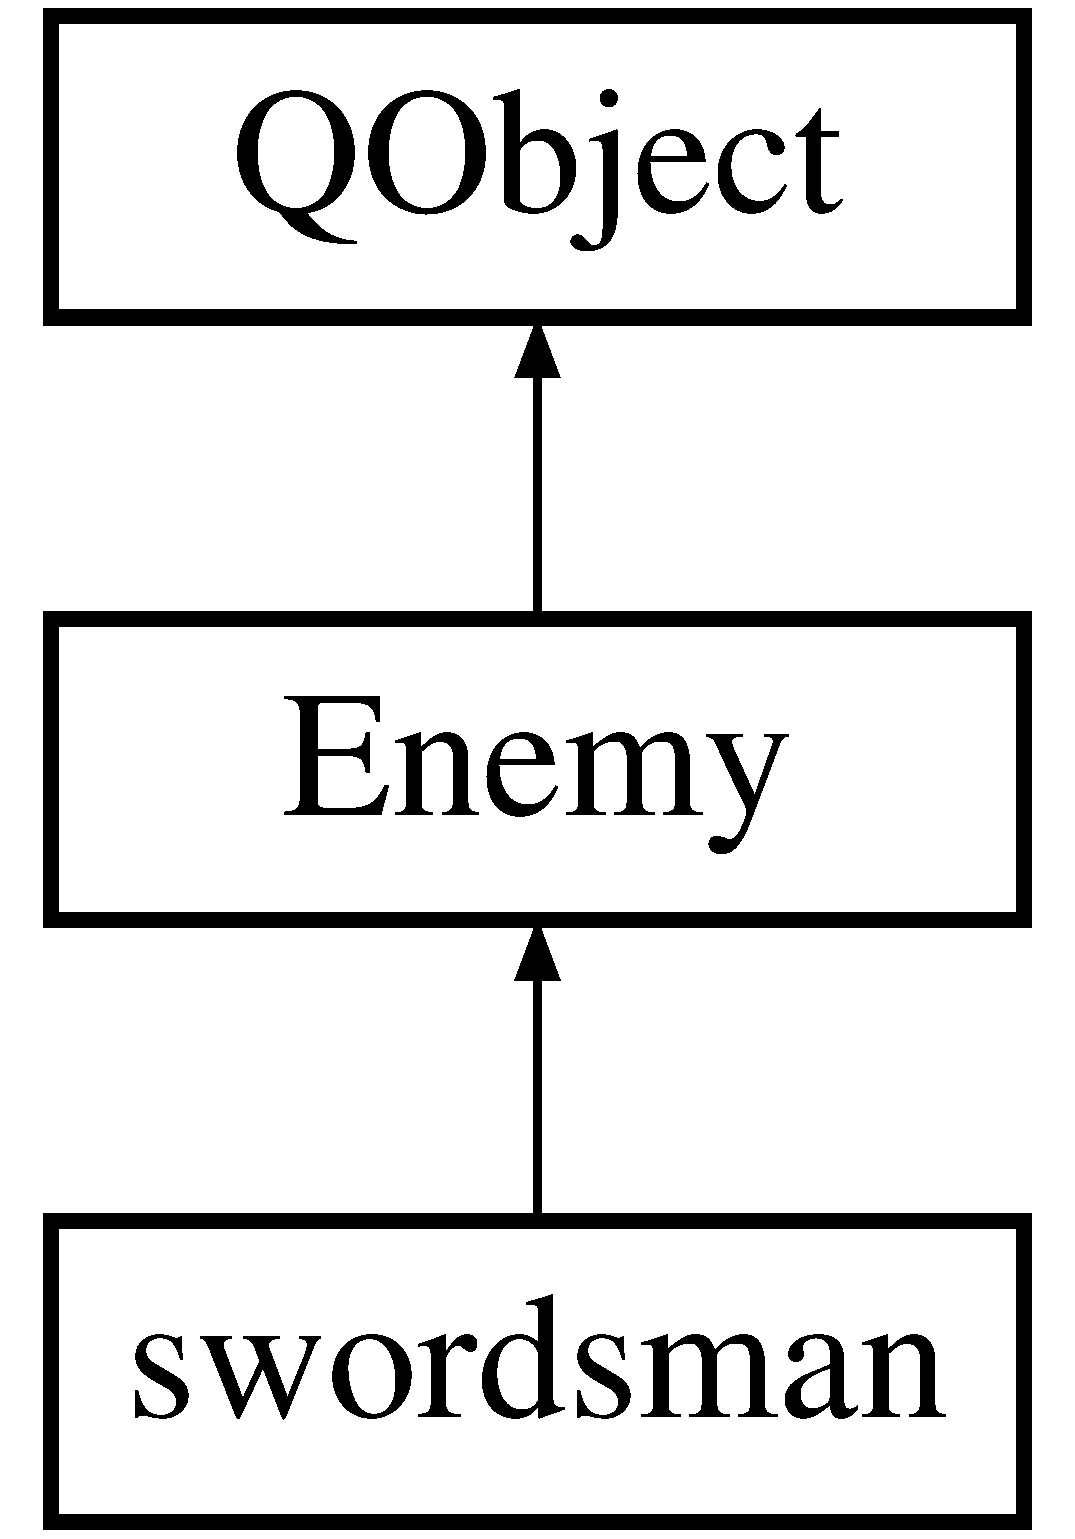
\includegraphics[height=3.000000cm]{classswordsman}
\end{center}
\end{figure}
\subsection*{Public Member Functions}
\begin{DoxyCompactItemize}
\item 
\hypertarget{classswordsman_afa4407146d49326932f9b1fa4f97ab2d}{{\bfseries swordsman} (int clev, int cx, int cy)}\label{classswordsman_afa4407146d49326932f9b1fa4f97ab2d}

\item 
virtual void \hyperlink{classswordsman_a99dec33c47dc5f3936229e5045b9c235}{do\-Turn} (\hyperlink{class_character}{Character} $\ast$Hero)
\begin{DoxyCompactList}\small\item\em \hyperlink{class_enemy_a56e4b9b07e8cd2a4e5ecfa8ff5b9265a}{Enemy\-::do\-Turn} based on hero's panel, does it's move. \end{DoxyCompactList}\item 
\hypertarget{classswordsman_a68098988c90a499ebfb757c7750bae7f}{virtual Q\-Image {\bfseries get\-Pic} ()}\label{classswordsman_a68098988c90a499ebfb757c7750bae7f}

\item 
virtual void \hyperlink{classswordsman_ad897e7c34033347faa5e4022b27cc395}{draw\-Self} (Q\-Painter $\ast$g, int gx, int gy)
\begin{DoxyCompactList}\small\item\em \hyperlink{class_enemy_a3251244e8e7ac657687d6be5a8da71bb}{Enemy\-::draw\-Self} draws itself using painter, includes title and hp. \end{DoxyCompactList}\end{DoxyCompactItemize}
\subsection*{Additional Inherited Members}


\subsection{Member Function Documentation}
\hypertarget{classswordsman_a99dec33c47dc5f3936229e5045b9c235}{\index{swordsman@{swordsman}!do\-Turn@{do\-Turn}}
\index{do\-Turn@{do\-Turn}!swordsman@{swordsman}}
\subsubsection[{do\-Turn}]{\setlength{\rightskip}{0pt plus 5cm}void swordsman\-::do\-Turn (
\begin{DoxyParamCaption}
\item[{{\bf Character} $\ast$}]{Hero}
\end{DoxyParamCaption}
)\hspace{0.3cm}{\ttfamily [virtual]}}}\label{classswordsman_a99dec33c47dc5f3936229e5045b9c235}


\hyperlink{class_enemy_a56e4b9b07e8cd2a4e5ecfa8ff5b9265a}{Enemy\-::do\-Turn} based on hero's panel, does it's move. 


\begin{DoxyParams}{Parameters}
{\em Hero} & \\
\hline
\end{DoxyParams}


Reimplemented from \hyperlink{class_enemy_a56e4b9b07e8cd2a4e5ecfa8ff5b9265a}{Enemy}.

\hypertarget{classswordsman_ad897e7c34033347faa5e4022b27cc395}{\index{swordsman@{swordsman}!draw\-Self@{draw\-Self}}
\index{draw\-Self@{draw\-Self}!swordsman@{swordsman}}
\subsubsection[{draw\-Self}]{\setlength{\rightskip}{0pt plus 5cm}void swordsman\-::draw\-Self (
\begin{DoxyParamCaption}
\item[{Q\-Painter $\ast$}]{g, }
\item[{int}]{gx, }
\item[{int}]{gy}
\end{DoxyParamCaption}
)\hspace{0.3cm}{\ttfamily [virtual]}}}\label{classswordsman_ad897e7c34033347faa5e4022b27cc395}


\hyperlink{class_enemy_a3251244e8e7ac657687d6be5a8da71bb}{Enemy\-::draw\-Self} draws itself using painter, includes title and hp. 


\begin{DoxyParams}{Parameters}
{\em g} & \\
\hline
{\em gx} & \\
\hline
{\em gy} & \\
\hline
\end{DoxyParams}


Reimplemented from \hyperlink{class_enemy_a3251244e8e7ac657687d6be5a8da71bb}{Enemy}.



The documentation for this class was generated from the following files\-:\begin{DoxyCompactItemize}
\item 
swordsman.\-h\item 
swordsman.\-cpp\end{DoxyCompactItemize}

\hypertarget{class_to_end}{\section{To\-End Class Reference}
\label{class_to_end}\index{To\-End@{To\-End}}
}
Inheritance diagram for To\-End\-:\begin{figure}[H]
\begin{center}
\leavevmode
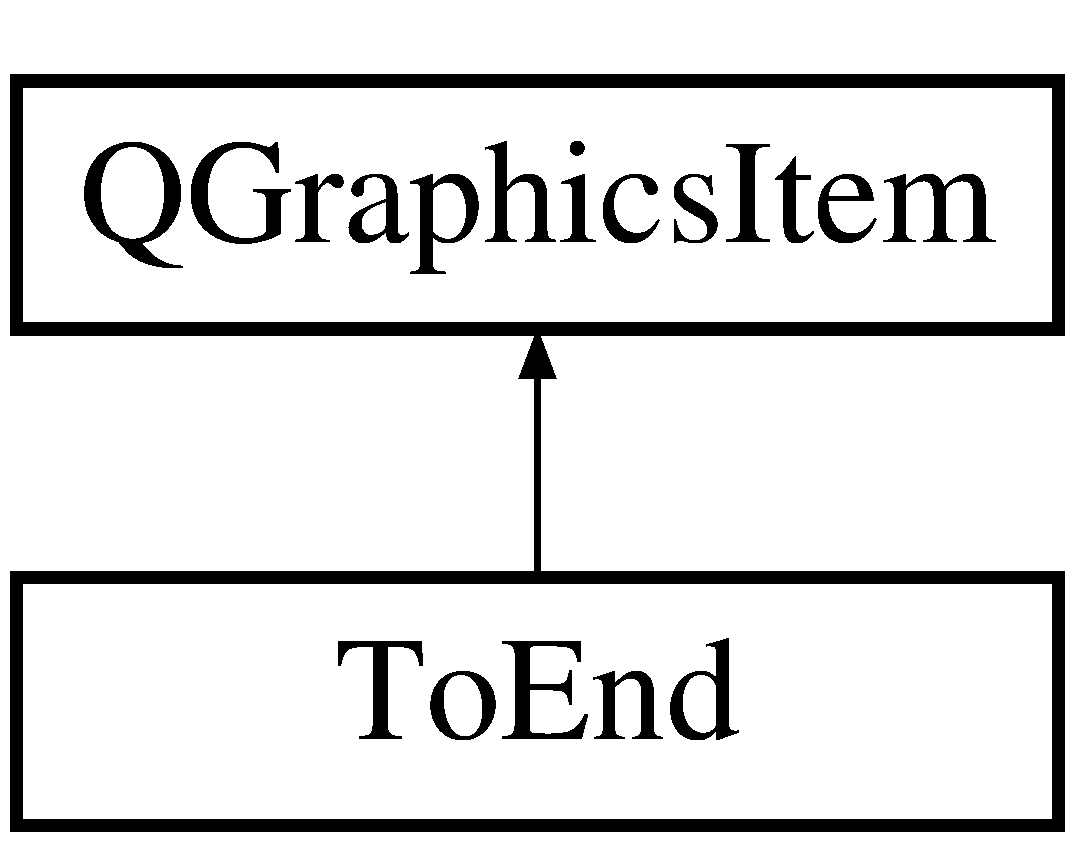
\includegraphics[height=2.000000cm]{class_to_end}
\end{center}
\end{figure}
\subsection*{Public Member Functions}
\begin{DoxyCompactItemize}
\item 
\hyperlink{class_to_end_a3581753bcd93c6124cede301373eec4b}{To\-End} (Q\-Graphics\-Item $\ast$parent=N\-U\-L\-L)
\begin{DoxyCompactList}\small\item\em \hyperlink{class_to_end_a3581753bcd93c6124cede301373eec4b}{To\-End\-::\-To\-End}. \end{DoxyCompactList}\item 
void \hyperlink{class_to_end_a8f9864d32e58c3cf2204299e63bbeeda}{paint} (Q\-Painter $\ast$painter, const Q\-Style\-Option\-Graphics\-Item $\ast$option, Q\-Widget $\ast$widget)
\begin{DoxyCompactList}\small\item\em \hyperlink{class_to_end_a8f9864d32e58c3cf2204299e63bbeeda}{To\-End\-::paint} the image. \end{DoxyCompactList}\item 
\hypertarget{class_to_end_aada516ddbf070dd4e961b3a49a242a0c}{\hyperlink{class_to_end_aada516ddbf070dd4e961b3a49a242a0c}{$\sim$\-To\-End} ()}\label{class_to_end_aada516ddbf070dd4e961b3a49a242a0c}

\begin{DoxyCompactList}\small\item\em \hyperlink{class_to_end_aada516ddbf070dd4e961b3a49a242a0c}{To\-End\-::$\sim$\-To\-End}. \end{DoxyCompactList}\end{DoxyCompactItemize}
\subsection*{Protected Member Functions}
\begin{DoxyCompactItemize}
\item 
Q\-Rect\-F \hyperlink{class_to_end_aea9d7014cf3c55fbabe5d28b621bc2f9}{bounding\-Rect} () const 
\begin{DoxyCompactList}\small\item\em \hyperlink{class_to_end_aea9d7014cf3c55fbabe5d28b621bc2f9}{To\-End\-::bounding\-Rect}. \end{DoxyCompactList}\end{DoxyCompactItemize}


\subsection{Constructor \& Destructor Documentation}
\hypertarget{class_to_end_a3581753bcd93c6124cede301373eec4b}{\index{To\-End@{To\-End}!To\-End@{To\-End}}
\index{To\-End@{To\-End}!ToEnd@{To\-End}}
\subsubsection[{To\-End}]{\setlength{\rightskip}{0pt plus 5cm}To\-End\-::\-To\-End (
\begin{DoxyParamCaption}
\item[{Q\-Graphics\-Item $\ast$}]{parent = {\ttfamily NULL}}
\end{DoxyParamCaption}
)}}\label{class_to_end_a3581753bcd93c6124cede301373eec4b}


\hyperlink{class_to_end_a3581753bcd93c6124cede301373eec4b}{To\-End\-::\-To\-End}. 


\begin{DoxyParams}{Parameters}
{\em parent} & \\
\hline
\end{DoxyParams}


\subsection{Member Function Documentation}
\hypertarget{class_to_end_aea9d7014cf3c55fbabe5d28b621bc2f9}{\index{To\-End@{To\-End}!bounding\-Rect@{bounding\-Rect}}
\index{bounding\-Rect@{bounding\-Rect}!ToEnd@{To\-End}}
\subsubsection[{bounding\-Rect}]{\setlength{\rightskip}{0pt plus 5cm}Q\-Rect\-F To\-End\-::bounding\-Rect (
\begin{DoxyParamCaption}
{}
\end{DoxyParamCaption}
) const\hspace{0.3cm}{\ttfamily [protected]}}}\label{class_to_end_aea9d7014cf3c55fbabe5d28b621bc2f9}


\hyperlink{class_to_end_aea9d7014cf3c55fbabe5d28b621bc2f9}{To\-End\-::bounding\-Rect}. 

\begin{DoxyReturn}{Returns}

\end{DoxyReturn}
\hypertarget{class_to_end_a8f9864d32e58c3cf2204299e63bbeeda}{\index{To\-End@{To\-End}!paint@{paint}}
\index{paint@{paint}!ToEnd@{To\-End}}
\subsubsection[{paint}]{\setlength{\rightskip}{0pt plus 5cm}void To\-End\-::paint (
\begin{DoxyParamCaption}
\item[{Q\-Painter $\ast$}]{painter, }
\item[{const Q\-Style\-Option\-Graphics\-Item $\ast$}]{option, }
\item[{Q\-Widget $\ast$}]{widget}
\end{DoxyParamCaption}
)}}\label{class_to_end_a8f9864d32e58c3cf2204299e63bbeeda}


\hyperlink{class_to_end_a8f9864d32e58c3cf2204299e63bbeeda}{To\-End\-::paint} the image. 


\begin{DoxyParams}{Parameters}
{\em painter} & \\
\hline
{\em option} & \\
\hline
{\em widget} & \\
\hline
\end{DoxyParams}


The documentation for this class was generated from the following files\-:\begin{DoxyCompactItemize}
\item 
toend.\-h\item 
toend.\-cpp\end{DoxyCompactItemize}

\hypertarget{class_to_store}{\section{To\-Store Class Reference}
\label{class_to_store}\index{To\-Store@{To\-Store}}
}
Inheritance diagram for To\-Store\-:\begin{figure}[H]
\begin{center}
\leavevmode
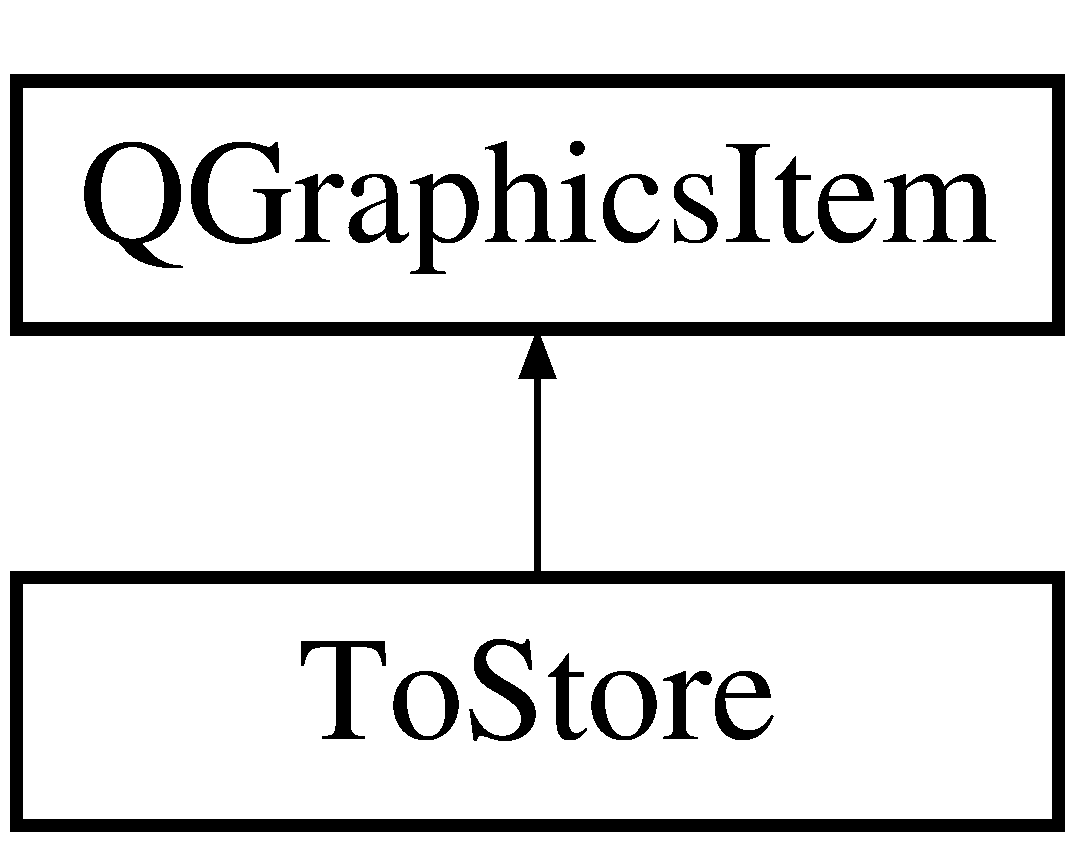
\includegraphics[height=2.000000cm]{class_to_store}
\end{center}
\end{figure}
\subsection*{Public Member Functions}
\begin{DoxyCompactItemize}
\item 
\hyperlink{class_to_store_a779ebd6b15419c4344946ce5b2a0064f}{To\-Store} (Q\-Graphics\-Item $\ast$parent=N\-U\-L\-L)
\begin{DoxyCompactList}\small\item\em \hyperlink{class_to_store_a779ebd6b15419c4344946ce5b2a0064f}{To\-Store\-::\-To\-Store}. \end{DoxyCompactList}\item 
void \hyperlink{class_to_store_aafd1a71a2edb0aae214a6747ce83a2bc}{paint} (Q\-Painter $\ast$painter, const Q\-Style\-Option\-Graphics\-Item $\ast$option, Q\-Widget $\ast$widget)
\begin{DoxyCompactList}\small\item\em To\-Store\-::paints the image item. \end{DoxyCompactList}\item 
\hypertarget{class_to_store_a8d4e9f0a522b741f24f6bc404457bd83}{\hyperlink{class_to_store_a8d4e9f0a522b741f24f6bc404457bd83}{$\sim$\-To\-Store} ()}\label{class_to_store_a8d4e9f0a522b741f24f6bc404457bd83}

\begin{DoxyCompactList}\small\item\em \hyperlink{class_to_store_a8d4e9f0a522b741f24f6bc404457bd83}{To\-Store\-::$\sim$\-To\-Store}. \end{DoxyCompactList}\end{DoxyCompactItemize}
\subsection*{Protected Member Functions}
\begin{DoxyCompactItemize}
\item 
Q\-Rect\-F \hyperlink{class_to_store_af17b0a3eea84d213fe09d2c503ab63db}{bounding\-Rect} () const 
\begin{DoxyCompactList}\small\item\em \hyperlink{class_to_store_af17b0a3eea84d213fe09d2c503ab63db}{To\-Store\-::bounding\-Rect}. \end{DoxyCompactList}\end{DoxyCompactItemize}


\subsection{Constructor \& Destructor Documentation}
\hypertarget{class_to_store_a779ebd6b15419c4344946ce5b2a0064f}{\index{To\-Store@{To\-Store}!To\-Store@{To\-Store}}
\index{To\-Store@{To\-Store}!ToStore@{To\-Store}}
\subsubsection[{To\-Store}]{\setlength{\rightskip}{0pt plus 5cm}To\-Store\-::\-To\-Store (
\begin{DoxyParamCaption}
\item[{Q\-Graphics\-Item $\ast$}]{parent = {\ttfamily NULL}}
\end{DoxyParamCaption}
)}}\label{class_to_store_a779ebd6b15419c4344946ce5b2a0064f}


\hyperlink{class_to_store_a779ebd6b15419c4344946ce5b2a0064f}{To\-Store\-::\-To\-Store}. 


\begin{DoxyParams}{Parameters}
{\em parent} & \\
\hline
\end{DoxyParams}


\subsection{Member Function Documentation}
\hypertarget{class_to_store_af17b0a3eea84d213fe09d2c503ab63db}{\index{To\-Store@{To\-Store}!bounding\-Rect@{bounding\-Rect}}
\index{bounding\-Rect@{bounding\-Rect}!ToStore@{To\-Store}}
\subsubsection[{bounding\-Rect}]{\setlength{\rightskip}{0pt plus 5cm}Q\-Rect\-F To\-Store\-::bounding\-Rect (
\begin{DoxyParamCaption}
{}
\end{DoxyParamCaption}
) const\hspace{0.3cm}{\ttfamily [protected]}}}\label{class_to_store_af17b0a3eea84d213fe09d2c503ab63db}


\hyperlink{class_to_store_af17b0a3eea84d213fe09d2c503ab63db}{To\-Store\-::bounding\-Rect}. 

\begin{DoxyReturn}{Returns}

\end{DoxyReturn}
\hypertarget{class_to_store_aafd1a71a2edb0aae214a6747ce83a2bc}{\index{To\-Store@{To\-Store}!paint@{paint}}
\index{paint@{paint}!ToStore@{To\-Store}}
\subsubsection[{paint}]{\setlength{\rightskip}{0pt plus 5cm}void To\-Store\-::paint (
\begin{DoxyParamCaption}
\item[{Q\-Painter $\ast$}]{painter, }
\item[{const Q\-Style\-Option\-Graphics\-Item $\ast$}]{option, }
\item[{Q\-Widget $\ast$}]{widget}
\end{DoxyParamCaption}
)}}\label{class_to_store_aafd1a71a2edb0aae214a6747ce83a2bc}


To\-Store\-::paints the image item. 


\begin{DoxyParams}{Parameters}
{\em painter} & \\
\hline
{\em option} & \\
\hline
{\em widget} & \\
\hline
\end{DoxyParams}


The documentation for this class was generated from the following files\-:\begin{DoxyCompactItemize}
\item 
tostore.\-h\item 
tostore.\-cpp\end{DoxyCompactItemize}

\hypertarget{class_ui___battle_pause}{\section{Ui\-\_\-\-Battle\-Pause Class Reference}
\label{class_ui___battle_pause}\index{Ui\-\_\-\-Battle\-Pause@{Ui\-\_\-\-Battle\-Pause}}
}
Inheritance diagram for Ui\-\_\-\-Battle\-Pause\-:\begin{figure}[H]
\begin{center}
\leavevmode
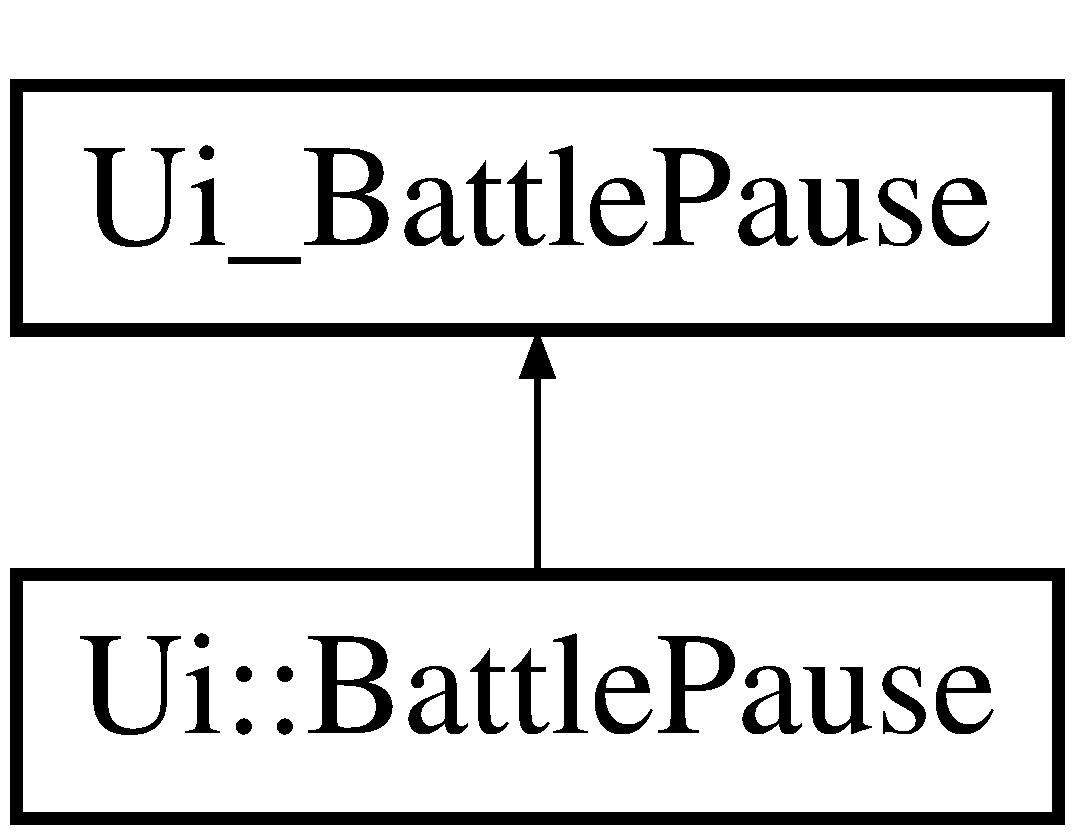
\includegraphics[height=2.000000cm]{class_ui___battle_pause}
\end{center}
\end{figure}
\subsection*{Public Member Functions}
\begin{DoxyCompactItemize}
\item 
\hypertarget{class_ui___battle_pause_a6d027885b86492cf6f99da870adb1e68}{void {\bfseries setup\-Ui} (Q\-Dialog $\ast$Battle\-Pause)}\label{class_ui___battle_pause_a6d027885b86492cf6f99da870adb1e68}

\item 
\hypertarget{class_ui___battle_pause_aea959080eab63120c832d9e0ff8309e1}{void {\bfseries retranslate\-Ui} (Q\-Dialog $\ast$Battle\-Pause)}\label{class_ui___battle_pause_aea959080eab63120c832d9e0ff8309e1}

\end{DoxyCompactItemize}
\subsection*{Public Attributes}
\begin{DoxyCompactItemize}
\item 
\hypertarget{class_ui___battle_pause_ad8006d9ba02a53c9c9003883f0e16a66}{Q\-Widget $\ast$ {\bfseries centralwidget}}\label{class_ui___battle_pause_ad8006d9ba02a53c9c9003883f0e16a66}

\item 
\hypertarget{class_ui___battle_pause_aaf264b9928c15ee8ac428eeb03593b74}{Q\-Label $\ast$ {\bfseries Pirate}}\label{class_ui___battle_pause_aaf264b9928c15ee8ac428eeb03593b74}

\item 
\hypertarget{class_ui___battle_pause_ac52cbf9d30b48c456c7d8016b3f2d5c9}{Q\-Push\-Button $\ast$ {\bfseries push\-Button}}\label{class_ui___battle_pause_ac52cbf9d30b48c456c7d8016b3f2d5c9}

\end{DoxyCompactItemize}


The documentation for this class was generated from the following file\-:\begin{DoxyCompactItemize}
\item 
ui\-\_\-battlepause.\-h\end{DoxyCompactItemize}

\hypertarget{class_ui___main_window}{\section{Ui\-\_\-\-Main\-Window Class Reference}
\label{class_ui___main_window}\index{Ui\-\_\-\-Main\-Window@{Ui\-\_\-\-Main\-Window}}
}
Inheritance diagram for Ui\-\_\-\-Main\-Window\-:\begin{figure}[H]
\begin{center}
\leavevmode
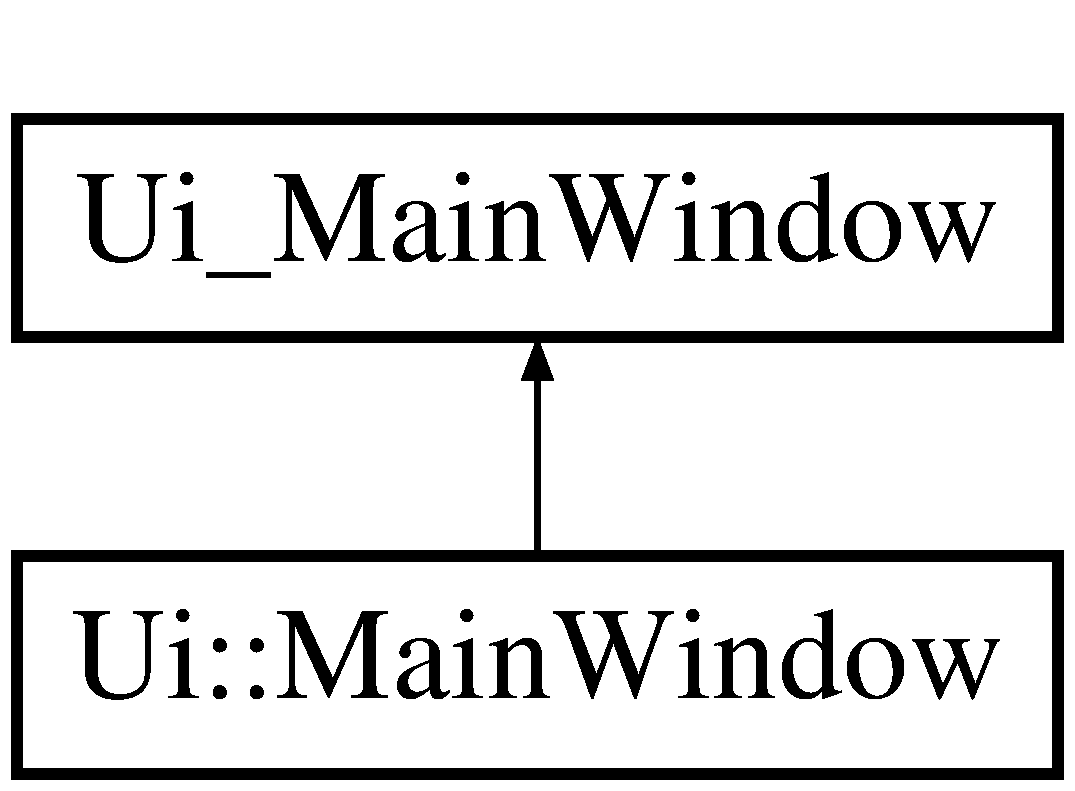
\includegraphics[height=2.000000cm]{class_ui___main_window}
\end{center}
\end{figure}
\subsection*{Public Member Functions}
\begin{DoxyCompactItemize}
\item 
\hypertarget{class_ui___main_window_acf4a0872c4c77d8f43a2ec66ed849b58}{void {\bfseries setup\-Ui} (Q\-Main\-Window $\ast$\hyperlink{class_main_window}{Main\-Window})}\label{class_ui___main_window_acf4a0872c4c77d8f43a2ec66ed849b58}

\item 
\hypertarget{class_ui___main_window_a097dd160c3534a204904cb374412c618}{void {\bfseries retranslate\-Ui} (Q\-Main\-Window $\ast$\hyperlink{class_main_window}{Main\-Window})}\label{class_ui___main_window_a097dd160c3534a204904cb374412c618}

\end{DoxyCompactItemize}
\subsection*{Public Attributes}
\begin{DoxyCompactItemize}
\item 
\hypertarget{class_ui___main_window_a30075506c2116c3ed4ff25e07ae75f81}{Q\-Widget $\ast$ {\bfseries central\-Widget}}\label{class_ui___main_window_a30075506c2116c3ed4ff25e07ae75f81}

\item 
\hypertarget{class_ui___main_window_ab676f235c393f334b7c07935d4007925}{Q\-Widget $\ast$ {\bfseries widget}}\label{class_ui___main_window_ab676f235c393f334b7c07935d4007925}

\item 
\hypertarget{class_ui___main_window_a80867018070156432923d0266cc9fe25}{Q\-H\-Box\-Layout $\ast$ {\bfseries horizontal\-Layout\-\_\-2}}\label{class_ui___main_window_a80867018070156432923d0266cc9fe25}

\item 
\hypertarget{class_ui___main_window_ad332d93084584930878f1daf5f84cdbf}{Q\-Push\-Button $\ast$ {\bfseries push\-Button}}\label{class_ui___main_window_ad332d93084584930878f1daf5f84cdbf}

\item 
\hypertarget{class_ui___main_window_acd6fdc9ebacc4b25b834162380d75ce8}{Q\-H\-Box\-Layout $\ast$ {\bfseries horizontal\-Layout}}\label{class_ui___main_window_acd6fdc9ebacc4b25b834162380d75ce8}

\item 
\hypertarget{class_ui___main_window_ac92cce0478c1025ace05ff4f8870bb1c}{Q\-Push\-Button $\ast$ {\bfseries push\-Button\-\_\-3}}\label{class_ui___main_window_ac92cce0478c1025ace05ff4f8870bb1c}

\item 
\hypertarget{class_ui___main_window_a59a7d8124bce933d63f53f2153d447b4}{Q\-Push\-Button $\ast$ {\bfseries push\-Button\-\_\-2}}\label{class_ui___main_window_a59a7d8124bce933d63f53f2153d447b4}

\item 
\hypertarget{class_ui___main_window_acb0b2f196dc2224f287b67594233297f}{Q\-Push\-Button $\ast$ {\bfseries push\-Button\-\_\-4}}\label{class_ui___main_window_acb0b2f196dc2224f287b67594233297f}

\item 
\hypertarget{class_ui___main_window_a2be1c24ec9adfca18e1dcc951931457f}{Q\-Menu\-Bar $\ast$ {\bfseries menu\-Bar}}\label{class_ui___main_window_a2be1c24ec9adfca18e1dcc951931457f}

\item 
\hypertarget{class_ui___main_window_a5172877001c8c7b4e0f6de50421867d1}{Q\-Tool\-Bar $\ast$ {\bfseries main\-Tool\-Bar}}\label{class_ui___main_window_a5172877001c8c7b4e0f6de50421867d1}

\item 
\hypertarget{class_ui___main_window_a50fa481337604bcc8bf68de18ab16ecd}{Q\-Status\-Bar $\ast$ {\bfseries status\-Bar}}\label{class_ui___main_window_a50fa481337604bcc8bf68de18ab16ecd}

\end{DoxyCompactItemize}


The documentation for this class was generated from the following file\-:\begin{DoxyCompactItemize}
\item 
ui\-\_\-mainwindow.\-h\end{DoxyCompactItemize}

\hypertarget{class_ui___pause}{\section{Ui\-\_\-\-Pause Class Reference}
\label{class_ui___pause}\index{Ui\-\_\-\-Pause@{Ui\-\_\-\-Pause}}
}
Inheritance diagram for Ui\-\_\-\-Pause\-:\begin{figure}[H]
\begin{center}
\leavevmode
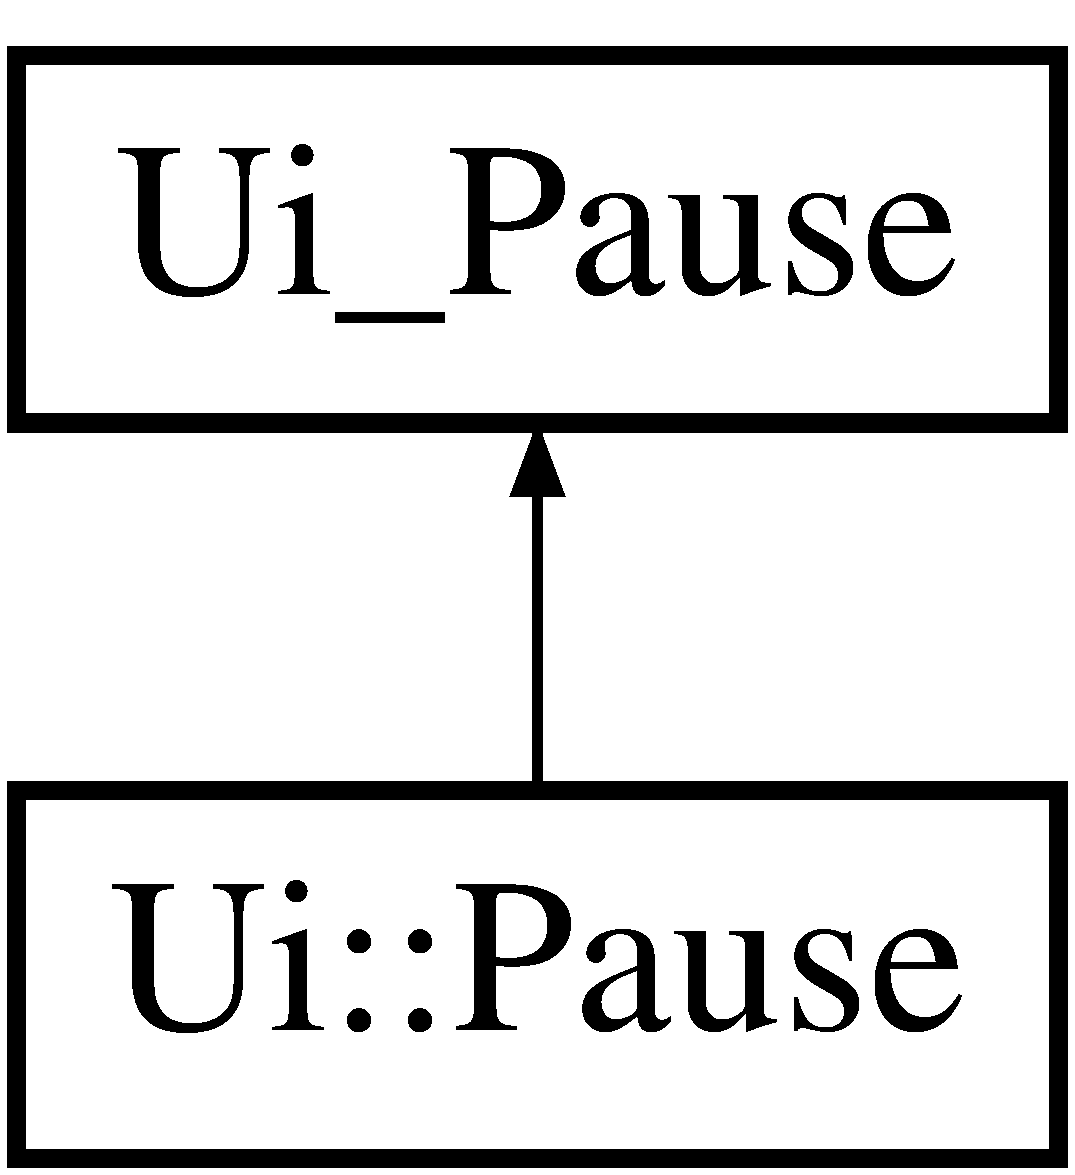
\includegraphics[height=2.000000cm]{class_ui___pause}
\end{center}
\end{figure}
\subsection*{Public Member Functions}
\begin{DoxyCompactItemize}
\item 
\hypertarget{class_ui___pause_af60e3e93c9c9c38a158724db32d41028}{void {\bfseries setup\-Ui} (Q\-Dialog $\ast$\hyperlink{class_pause}{Pause})}\label{class_ui___pause_af60e3e93c9c9c38a158724db32d41028}

\item 
\hypertarget{class_ui___pause_a6ffdb8372507fe77e7de36b822e30da1}{void {\bfseries retranslate\-Ui} (Q\-Dialog $\ast$\hyperlink{class_pause}{Pause})}\label{class_ui___pause_a6ffdb8372507fe77e7de36b822e30da1}

\end{DoxyCompactItemize}
\subsection*{Public Attributes}
\begin{DoxyCompactItemize}
\item 
\hypertarget{class_ui___pause_a98e7c02b762002d5e49cc11a19216c92}{Q\-Label $\ast$ {\bfseries pirate}}\label{class_ui___pause_a98e7c02b762002d5e49cc11a19216c92}

\item 
\hypertarget{class_ui___pause_a0f6b437e2e11c35eeeb173afb55e2f41}{Q\-Progress\-Bar $\ast$ {\bfseries progress\-Bar}}\label{class_ui___pause_a0f6b437e2e11c35eeeb173afb55e2f41}

\item 
\hypertarget{class_ui___pause_ae853eb73f144e6070615a2c4135a0bd0}{Q\-L\-C\-D\-Number $\ast$ {\bfseries lcd\-Number}}\label{class_ui___pause_ae853eb73f144e6070615a2c4135a0bd0}

\item 
\hypertarget{class_ui___pause_a02cec35c8d610e79dfd365a735607677}{Q\-Tab\-Widget $\ast$ {\bfseries tab\-Widget}}\label{class_ui___pause_a02cec35c8d610e79dfd365a735607677}

\item 
\hypertarget{class_ui___pause_ae67cc2921986e434f664f728095ed411}{Q\-Widget $\ast$ {\bfseries tab}}\label{class_ui___pause_ae67cc2921986e434f664f728095ed411}

\item 
\hypertarget{class_ui___pause_aca1dc186997c10b10301ba2e8c8766d3}{Q\-Push\-Button $\ast$ {\bfseries inc\-Sword\-Damage}}\label{class_ui___pause_aca1dc186997c10b10301ba2e8c8766d3}

\item 
\hypertarget{class_ui___pause_aaa48eb0c33b3b5919743b29ca60739de}{Q\-Push\-Button $\ast$ {\bfseries inc\-Gun\-Damage}}\label{class_ui___pause_aaa48eb0c33b3b5919743b29ca60739de}

\item 
\hypertarget{class_ui___pause_ae0629b76fc9d2433159a991fd85a52b4}{Q\-Push\-Button $\ast$ {\bfseries inc\-Hook\-Damage}}\label{class_ui___pause_ae0629b76fc9d2433159a991fd85a52b4}

\item 
\hypertarget{class_ui___pause_ac1bbd23d8f3fba52d05eabe522e1de73}{Q\-Push\-Button $\ast$ {\bfseries inc\-Broken\-Gun\-Damage}}\label{class_ui___pause_ac1bbd23d8f3fba52d05eabe522e1de73}

\item 
\hypertarget{class_ui___pause_a90afc301cf509c97a33b7fcec631f87c}{Q\-Widget $\ast$ {\bfseries tab\-\_\-2}}\label{class_ui___pause_a90afc301cf509c97a33b7fcec631f87c}

\item 
\hypertarget{class_ui___pause_afd3556b54af701c2cf595d7143d65997}{Q\-Push\-Button $\ast$ {\bfseries restore\-Health}}\label{class_ui___pause_afd3556b54af701c2cf595d7143d65997}

\item 
\hypertarget{class_ui___pause_a874efa7bf05b6985b29194c524b9c0bf}{Q\-Push\-Button $\ast$ {\bfseries inc\-Health}}\label{class_ui___pause_a874efa7bf05b6985b29194c524b9c0bf}

\item 
\hypertarget{class_ui___pause_a952fd2960c5a1272ba25d09fe58db761}{Q\-Widget $\ast$ {\bfseries layout\-Widget}}\label{class_ui___pause_a952fd2960c5a1272ba25d09fe58db761}

\item 
\hypertarget{class_ui___pause_aba248dba2af7138a892f168ddf2c6bab}{Q\-H\-Box\-Layout $\ast$ {\bfseries horizontal\-Layout}}\label{class_ui___pause_aba248dba2af7138a892f168ddf2c6bab}

\item 
\hypertarget{class_ui___pause_a418e4f1b37ad8d68c20bd99514b96938}{Q\-Push\-Button $\ast$ {\bfseries resume}}\label{class_ui___pause_a418e4f1b37ad8d68c20bd99514b96938}

\item 
\hypertarget{class_ui___pause_a89df91a5abb4b5ac7f82f9362dca8315}{Q\-Spacer\-Item $\ast$ {\bfseries horizontal\-Spacer}}\label{class_ui___pause_a89df91a5abb4b5ac7f82f9362dca8315}

\item 
\hypertarget{class_ui___pause_a03665e15a7d5851e4ef871429140c900}{Q\-Push\-Button $\ast$ {\bfseries exit}}\label{class_ui___pause_a03665e15a7d5851e4ef871429140c900}

\end{DoxyCompactItemize}


The documentation for this class was generated from the following file\-:\begin{DoxyCompactItemize}
\item 
ui\-\_\-pause.\-h\end{DoxyCompactItemize}

\hypertarget{class_ui__worldmap}{\section{Ui\-\_\-worldmap Class Reference}
\label{class_ui__worldmap}\index{Ui\-\_\-worldmap@{Ui\-\_\-worldmap}}
}
Inheritance diagram for Ui\-\_\-worldmap\-:\begin{figure}[H]
\begin{center}
\leavevmode
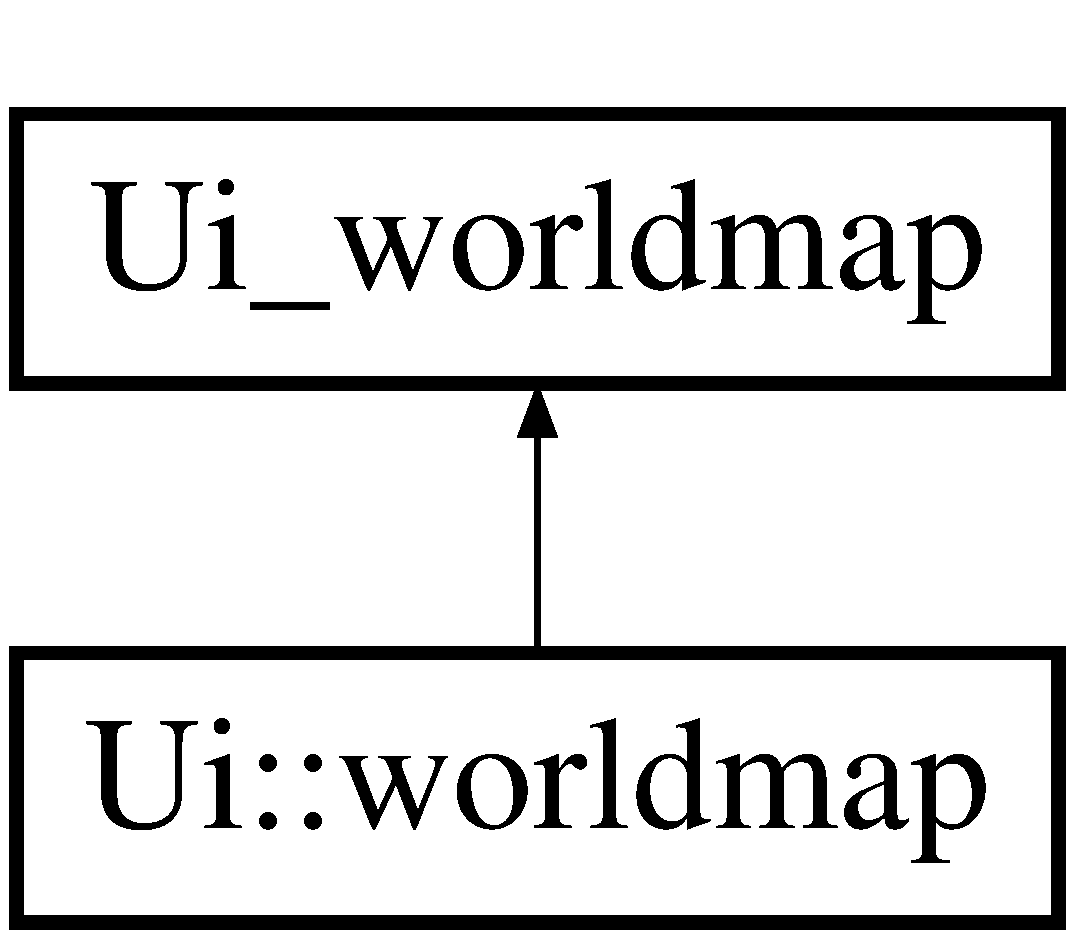
\includegraphics[height=2.000000cm]{class_ui__worldmap}
\end{center}
\end{figure}
\subsection*{Public Member Functions}
\begin{DoxyCompactItemize}
\item 
\hypertarget{class_ui__worldmap_ab7d2484e858585cb624fc3d3f0565c04}{void {\bfseries setup\-Ui} (Q\-Dialog $\ast$\hyperlink{classworldmap}{worldmap})}\label{class_ui__worldmap_ab7d2484e858585cb624fc3d3f0565c04}

\item 
\hypertarget{class_ui__worldmap_ad9a0a2c03f11c614814db6e90484a479}{void {\bfseries retranslate\-Ui} (Q\-Dialog $\ast$\hyperlink{classworldmap}{worldmap})}\label{class_ui__worldmap_ad9a0a2c03f11c614814db6e90484a479}

\end{DoxyCompactItemize}
\subsection*{Public Attributes}
\begin{DoxyCompactItemize}
\item 
\hypertarget{class_ui__worldmap_a2877c0f2062f90387f526cc98f78fadc}{Q\-Graphics\-View $\ast$ {\bfseries graphics\-View}}\label{class_ui__worldmap_a2877c0f2062f90387f526cc98f78fadc}

\item 
\hypertarget{class_ui__worldmap_aa1591d6b2978ebc1b8b1b3f9a89c5fae}{Q\-Push\-Button $\ast$ {\bfseries push\-Button}}\label{class_ui__worldmap_aa1591d6b2978ebc1b8b1b3f9a89c5fae}

\end{DoxyCompactItemize}


The documentation for this class was generated from the following file\-:\begin{DoxyCompactItemize}
\item 
ui\-\_\-worldmap.\-h\end{DoxyCompactItemize}

\hypertarget{class_wiggly_widget}{\section{Wiggly\-Widget Class Reference}
\label{class_wiggly_widget}\index{Wiggly\-Widget@{Wiggly\-Widget}}
}


\mbox{[}0\mbox{]}  




{\ttfamily \#include $<$wigglywidget.\-h$>$}

Inheritance diagram for Wiggly\-Widget\-:\begin{figure}[H]
\begin{center}
\leavevmode
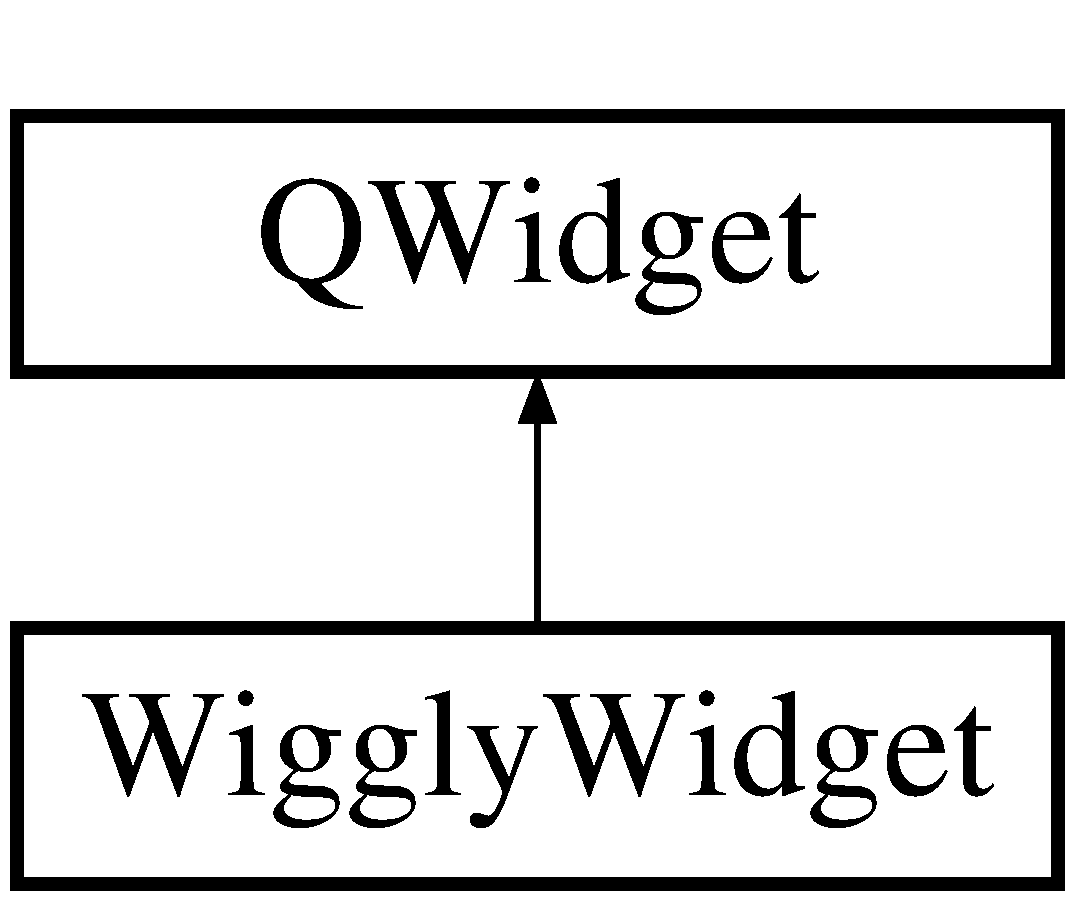
\includegraphics[height=2.000000cm]{class_wiggly_widget}
\end{center}
\end{figure}
\subsection*{Public Slots}
\begin{DoxyCompactItemize}
\item 
\hypertarget{class_wiggly_widget_ad5a15c8f2b92caff1ea0b2332bc33247}{void {\bfseries set\-Text} (const Q\-String \&new\-Text)}\label{class_wiggly_widget_ad5a15c8f2b92caff1ea0b2332bc33247}

\end{DoxyCompactItemize}
\subsection*{Public Member Functions}
\begin{DoxyCompactItemize}
\item 
\hypertarget{class_wiggly_widget_a01692879d180d866e26bc8a7463b5457}{\hyperlink{class_wiggly_widget_a01692879d180d866e26bc8a7463b5457}{Wiggly\-Widget} (int fontsize, Q\-Widget $\ast$parent=0)}\label{class_wiggly_widget_a01692879d180d866e26bc8a7463b5457}

\begin{DoxyCompactList}\small\item\em \mbox{[}0\mbox{]} \end{DoxyCompactList}\end{DoxyCompactItemize}
\subsection*{Protected Member Functions}
\begin{DoxyCompactItemize}
\item 
void \hyperlink{class_wiggly_widget_a23b24eab03ec0d6681ef44680957b6ce}{paint\-Event} (Q\-Paint\-Event $\ast$event)
\begin{DoxyCompactList}\small\item\em \mbox{[}0\mbox{]} \end{DoxyCompactList}\item 
void \hyperlink{class_wiggly_widget_a966bfc0c0f723b5b3b61ab939ca8006c}{timer\-Event} (Q\-Timer\-Event $\ast$event)
\begin{DoxyCompactList}\small\item\em \mbox{[}4\mbox{]} \end{DoxyCompactList}\end{DoxyCompactItemize}


\subsection{Detailed Description}
\mbox{[}0\mbox{]} 

\subsection{Member Function Documentation}
\hypertarget{class_wiggly_widget_a23b24eab03ec0d6681ef44680957b6ce}{\index{Wiggly\-Widget@{Wiggly\-Widget}!paint\-Event@{paint\-Event}}
\index{paint\-Event@{paint\-Event}!WigglyWidget@{Wiggly\-Widget}}
\subsubsection[{paint\-Event}]{\setlength{\rightskip}{0pt plus 5cm}void Wiggly\-Widget\-::paint\-Event (
\begin{DoxyParamCaption}
\item[{Q\-Paint\-Event $\ast$}]{event}
\end{DoxyParamCaption}
)\hspace{0.3cm}{\ttfamily [protected]}}}\label{class_wiggly_widget_a23b24eab03ec0d6681ef44680957b6ce}


\mbox{[}0\mbox{]} 

\mbox{[}1\mbox{]} \mbox{[}1\mbox{]} //! \mbox{[}2\mbox{]} \mbox{[}2\mbox{]}

\mbox{[}3\mbox{]}

\mbox{[}3\mbox{]} //! \mbox{[}4\mbox{]} \hypertarget{class_wiggly_widget_a966bfc0c0f723b5b3b61ab939ca8006c}{\index{Wiggly\-Widget@{Wiggly\-Widget}!timer\-Event@{timer\-Event}}
\index{timer\-Event@{timer\-Event}!WigglyWidget@{Wiggly\-Widget}}
\subsubsection[{timer\-Event}]{\setlength{\rightskip}{0pt plus 5cm}void Wiggly\-Widget\-::timer\-Event (
\begin{DoxyParamCaption}
\item[{Q\-Timer\-Event $\ast$}]{event}
\end{DoxyParamCaption}
)\hspace{0.3cm}{\ttfamily [protected]}}}\label{class_wiggly_widget_a966bfc0c0f723b5b3b61ab939ca8006c}


\mbox{[}4\mbox{]} 

\mbox{[}5\mbox{]} \mbox{[}5\mbox{]} //! \mbox{[}6\mbox{]} \mbox{[}6\mbox{]} 

The documentation for this class was generated from the following files\-:\begin{DoxyCompactItemize}
\item 
wigglywidget.\-h\item 
wigglywidget.\-cpp\end{DoxyCompactItemize}

\hypertarget{classworldmap}{\section{worldmap Class Reference}
\label{classworldmap}\index{worldmap@{worldmap}}
}
Inheritance diagram for worldmap\-:\begin{figure}[H]
\begin{center}
\leavevmode
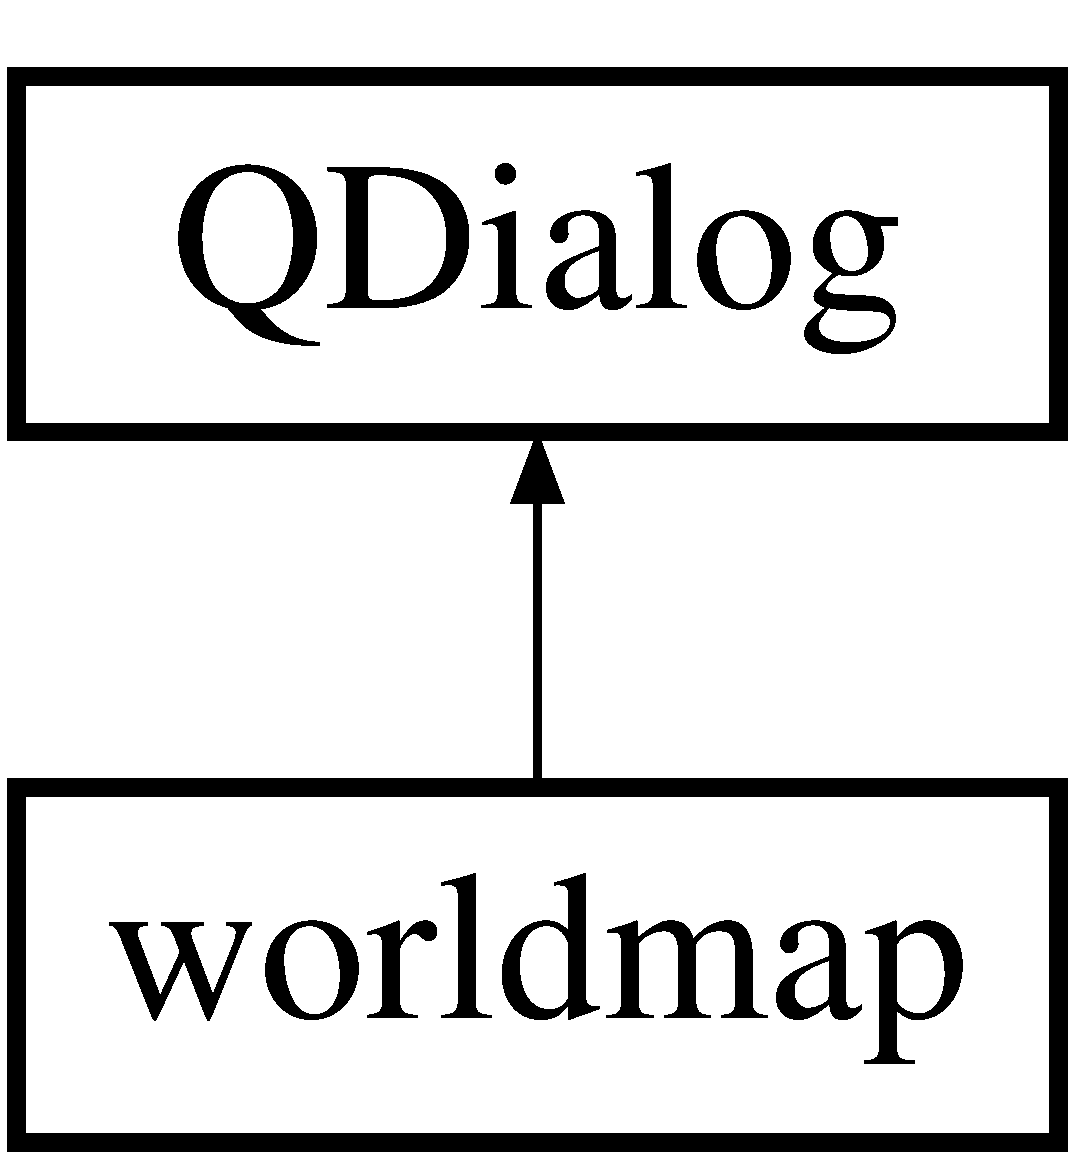
\includegraphics[height=2.000000cm]{classworldmap}
\end{center}
\end{figure}
\subsection*{Public Member Functions}
\begin{DoxyCompactItemize}
\item 
\hyperlink{classworldmap_a970f51f58c07cc43b110fecf43519838}{worldmap} (Q\-Widget $\ast$parent=0)
\begin{DoxyCompactList}\small\item\em \hyperlink{classworldmap_a970f51f58c07cc43b110fecf43519838}{worldmap\-::worldmap} \end{DoxyCompactList}\item 
\hypertarget{classworldmap_a3ae55f6ff120219ab10a80123cb8b537}{\hyperlink{classworldmap_a3ae55f6ff120219ab10a80123cb8b537}{$\sim$worldmap} ()}\label{classworldmap_a3ae55f6ff120219ab10a80123cb8b537}

\begin{DoxyCompactList}\small\item\em \hyperlink{classworldmap_a3ae55f6ff120219ab10a80123cb8b537}{worldmap\-::$\sim$worldmap} \end{DoxyCompactList}\end{DoxyCompactItemize}
\subsection*{Public Attributes}
\begin{DoxyCompactItemize}
\item 
\hypertarget{classworldmap_a5bb13c3e0f22ca81a28a5bbc59fb027a}{\hyperlink{class_ui_1_1worldmap}{Ui\-::worldmap} $\ast$ {\bfseries ui}}\label{classworldmap_a5bb13c3e0f22ca81a28a5bbc59fb027a}

\item 
\hypertarget{classworldmap_a0839b1d6d909275245a30e0b2772426c}{Q\-Graphics\-Scene $\ast$ {\bfseries scene1}}\label{classworldmap_a0839b1d6d909275245a30e0b2772426c}

\item 
\hypertarget{classworldmap_ad19dbf95b9ea420fefe6d1178d546cfc}{Q\-Graphics\-Scene $\ast$ {\bfseries scene2}}\label{classworldmap_ad19dbf95b9ea420fefe6d1178d546cfc}

\item 
\hypertarget{classworldmap_a5336dd95886020b89fc26dbaecbd780f}{Q\-Graphics\-Scene $\ast$ {\bfseries scene3}}\label{classworldmap_a5336dd95886020b89fc26dbaecbd780f}

\item 
\hypertarget{classworldmap_a2032fc999b6b2692e5e73ed5718f8252}{Q\-Graphics\-Scene $\ast$ {\bfseries scene4}}\label{classworldmap_a2032fc999b6b2692e5e73ed5718f8252}

\item 
\hypertarget{classworldmap_ad947cbd86ef3deff43d1c0206032c8e6}{\hyperlink{class_map_hero}{Map\-Hero} $\ast$ {\bfseries hero}}\label{classworldmap_ad947cbd86ef3deff43d1c0206032c8e6}

\item 
\hypertarget{classworldmap_ace4a35cb38e90cb5e46cf96fc46713c3}{\hyperlink{class_map_enemy}{Map\-Enemy} $\ast$ {\bfseries enemy}}\label{classworldmap_ace4a35cb38e90cb5e46cf96fc46713c3}

\item 
\hypertarget{classworldmap_a91f7cab38c03e01352a4b64547ade607}{\hyperlink{class_mini_enemy}{Mini\-Enemy} $\ast$ {\bfseries mini\-Enemy}}\label{classworldmap_a91f7cab38c03e01352a4b64547ade607}

\item 
\hypertarget{classworldmap_a2374997ed32ff5b460acbbf30e8e01b8}{\hyperlink{class_mega_enemy}{Mega\-Enemy} $\ast$ {\bfseries mega\-Enemy}}\label{classworldmap_a2374997ed32ff5b460acbbf30e8e01b8}

\item 
\hypertarget{classworldmap_a03d177209c0acff0a3607894048239b2}{\hyperlink{class_pause}{Pause} $\ast$ {\bfseries pause}}\label{classworldmap_a03d177209c0acff0a3607894048239b2}

\item 
\hypertarget{classworldmap_afa6000326057e72e56f346362edf7cae}{\hyperlink{class_to_store}{To\-Store} $\ast$ {\bfseries m\-Store}}\label{classworldmap_afa6000326057e72e56f346362edf7cae}

\item 
\hypertarget{classworldmap_a24cd3a687f3b97ef6fd56b2adc19fcdb}{\hyperlink{class_in_store}{In\-Store} $\ast$ {\bfseries n\-Store}}\label{classworldmap_a24cd3a687f3b97ef6fd56b2adc19fcdb}

\item 
\hypertarget{classworldmap_a13a123b334231979f5466d29a989c7cc}{\hyperlink{class_to_end}{To\-End} $\ast$ {\bfseries to\-End}}\label{classworldmap_a13a123b334231979f5466d29a989c7cc}

\item 
\hypertarget{classworldmap_a4a3da7e4dc049037fbe3f74414bce53f}{\hyperlink{class_back_from_in_store}{Back\-From\-In\-Store} $\ast$ {\bfseries from\-In\-Store}}\label{classworldmap_a4a3da7e4dc049037fbe3f74414bce53f}

\item 
\hypertarget{classworldmap_a4ae3ffd0704cb13058ef3413012c2663}{\hyperlink{class_back_from_store}{Back\-From\-Store} $\ast$ {\bfseries from\-Store}}\label{classworldmap_a4ae3ffd0704cb13058ef3413012c2663}

\item 
\hypertarget{classworldmap_a9d29b583239464b8b6a203831509fb3b}{\hyperlink{class_back_from_end}{Back\-From\-End} $\ast$ {\bfseries from\-End}}\label{classworldmap_a9d29b583239464b8b6a203831509fb3b}

\end{DoxyCompactItemize}


\subsection{Constructor \& Destructor Documentation}
\hypertarget{classworldmap_a970f51f58c07cc43b110fecf43519838}{\index{worldmap@{worldmap}!worldmap@{worldmap}}
\index{worldmap@{worldmap}!worldmap@{worldmap}}
\subsubsection[{worldmap}]{\setlength{\rightskip}{0pt plus 5cm}worldmap\-::worldmap (
\begin{DoxyParamCaption}
\item[{Q\-Widget $\ast$}]{parent = {\ttfamily 0}}
\end{DoxyParamCaption}
)\hspace{0.3cm}{\ttfamily [explicit]}}}\label{classworldmap_a970f51f58c07cc43b110fecf43519838}


\hyperlink{classworldmap_a970f51f58c07cc43b110fecf43519838}{worldmap\-::worldmap} 


\begin{DoxyParams}{Parameters}
{\em parent} & \\
\hline
\end{DoxyParams}


The documentation for this class was generated from the following files\-:\begin{DoxyCompactItemize}
\item 
worldmap.\-h\item 
worldmap.\-cpp\end{DoxyCompactItemize}

\hypertarget{class_ui_1_1worldmap}{\section{Ui\-:\-:worldmap Class Reference}
\label{class_ui_1_1worldmap}\index{Ui\-::worldmap@{Ui\-::worldmap}}
}
Inheritance diagram for Ui\-:\-:worldmap\-:\begin{figure}[H]
\begin{center}
\leavevmode
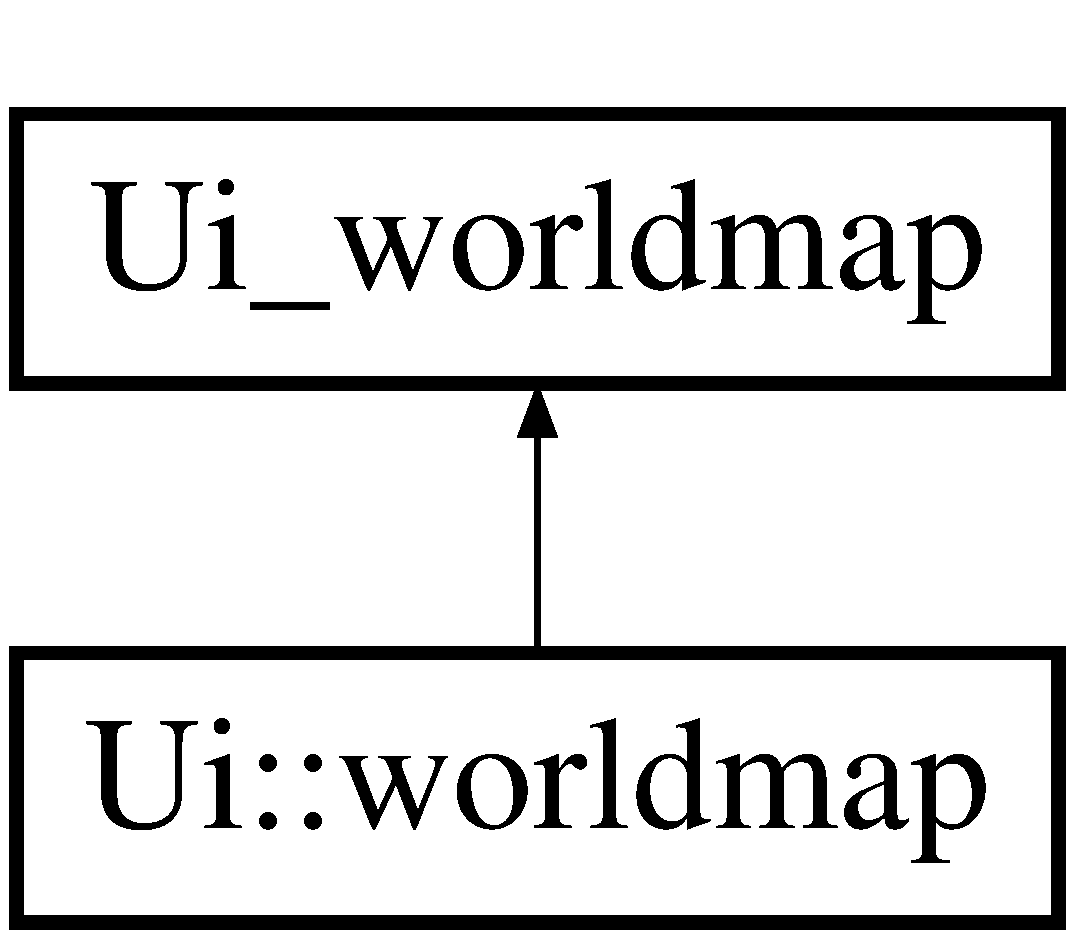
\includegraphics[height=2.000000cm]{class_ui_1_1worldmap}
\end{center}
\end{figure}
\subsection*{Additional Inherited Members}


The documentation for this class was generated from the following file\-:\begin{DoxyCompactItemize}
\item 
ui\-\_\-worldmap.\-h\end{DoxyCompactItemize}

\hypertarget{classxgun}{\section{xgun Class Reference}
\label{classxgun}\index{xgun@{xgun}}
}
Inheritance diagram for xgun\-:\begin{figure}[H]
\begin{center}
\leavevmode
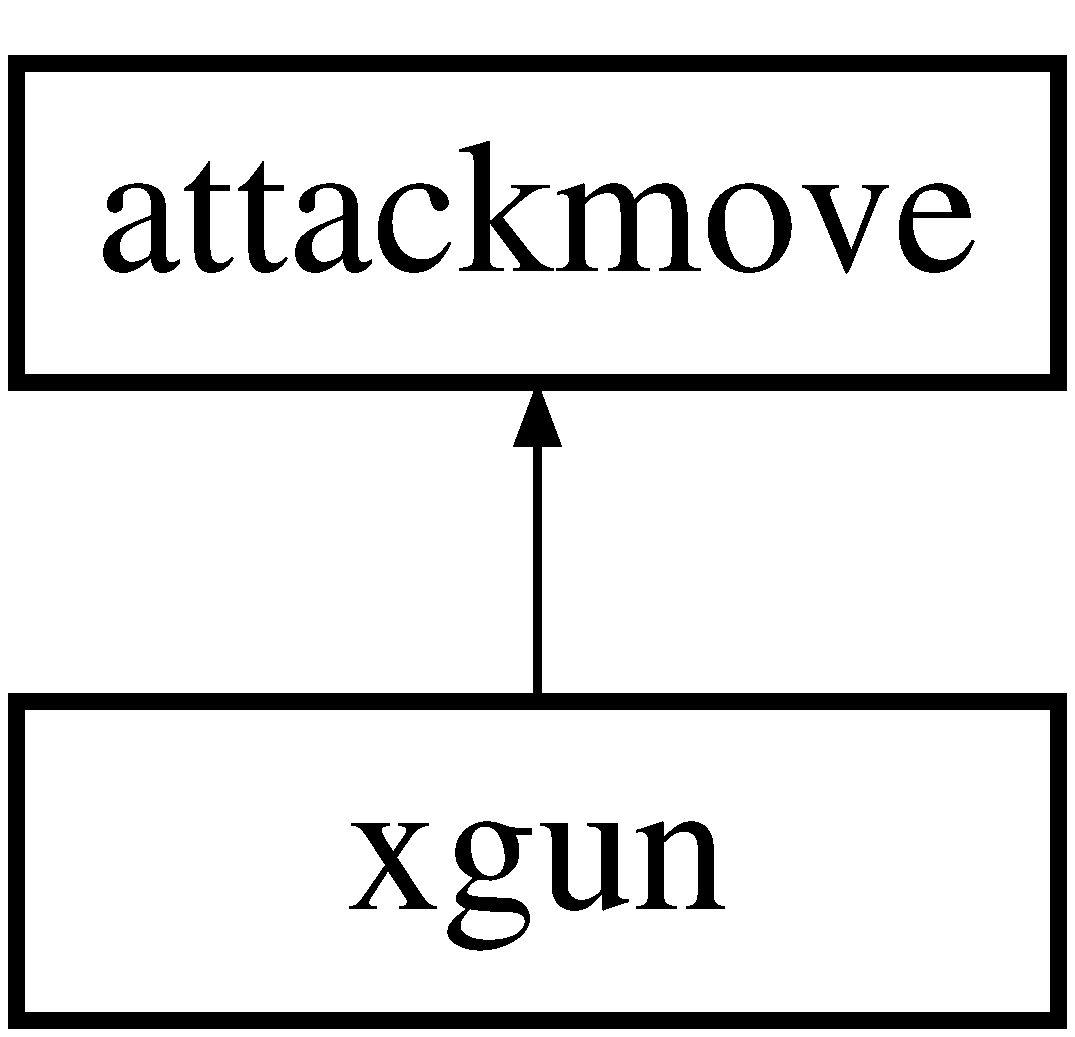
\includegraphics[height=2.000000cm]{classxgun}
\end{center}
\end{figure}
\subsection*{Public Member Functions}
\begin{DoxyCompactItemize}
\item 
\hypertarget{classxgun_a559665713dc1ae233184807d8b38ab7f}{{\bfseries xgun} (int dam)}\label{classxgun_a559665713dc1ae233184807d8b38ab7f}

\item 
virtual Q\-String \hyperlink{classxgun_a8d091859d655ff1703630ba7dd88a358}{get\-String} ()
\begin{DoxyCompactList}\small\item\em \hyperlink{classattackmove_ada49eedf4b893372c576edd48fe73161}{attackmove\-::get\-String} \end{DoxyCompactList}\item 
virtual Q\-Image \hyperlink{classxgun_adf5511bd6ed5dfb184a8a3b6b757608a}{get\-Image} ()
\begin{DoxyCompactList}\small\item\em \hyperlink{classattackmove_aca59a2343b7a6c195d300dda5c8d952d}{attackmove\-::get\-Image} \end{DoxyCompactList}\item 
\hypertarget{classxgun_aac799bda61860430dbbd9403b80a1efd}{virtual void {\bfseries get\-Hover} (int hpanel, \hyperlink{class_enemy}{Enemy} $\ast$Enemies\mbox{[}$\,$\mbox{]}, \hyperlink{classanim_items}{anim\-Items} $\ast$anim)}\label{classxgun_aac799bda61860430dbbd9403b80a1efd}

\item 
\hypertarget{classxgun_a8ede91a770bcedc6c4454615d38b5e84}{virtual void {\bfseries do\-Attack} (int hpanel, \hyperlink{class_enemy}{Enemy} $\ast$Enemies\mbox{[}$\,$\mbox{]}, \hyperlink{classanim_items}{anim\-Items} $\ast$anim)}\label{classxgun_a8ede91a770bcedc6c4454615d38b5e84}

\end{DoxyCompactItemize}
\subsection*{Additional Inherited Members}


\subsection{Member Function Documentation}
\hypertarget{classxgun_adf5511bd6ed5dfb184a8a3b6b757608a}{\index{xgun@{xgun}!get\-Image@{get\-Image}}
\index{get\-Image@{get\-Image}!xgun@{xgun}}
\subsubsection[{get\-Image}]{\setlength{\rightskip}{0pt plus 5cm}Q\-Image xgun\-::get\-Image (
\begin{DoxyParamCaption}
{}
\end{DoxyParamCaption}
)\hspace{0.3cm}{\ttfamily [virtual]}}}\label{classxgun_adf5511bd6ed5dfb184a8a3b6b757608a}


\hyperlink{classattackmove_aca59a2343b7a6c195d300dda5c8d952d}{attackmove\-::get\-Image} 

\begin{DoxyReturn}{Returns}

\end{DoxyReturn}


Reimplemented from \hyperlink{classattackmove_aca59a2343b7a6c195d300dda5c8d952d}{attackmove}.

\hypertarget{classxgun_a8d091859d655ff1703630ba7dd88a358}{\index{xgun@{xgun}!get\-String@{get\-String}}
\index{get\-String@{get\-String}!xgun@{xgun}}
\subsubsection[{get\-String}]{\setlength{\rightskip}{0pt plus 5cm}Q\-String xgun\-::get\-String (
\begin{DoxyParamCaption}
{}
\end{DoxyParamCaption}
)\hspace{0.3cm}{\ttfamily [virtual]}}}\label{classxgun_a8d091859d655ff1703630ba7dd88a358}


\hyperlink{classattackmove_ada49eedf4b893372c576edd48fe73161}{attackmove\-::get\-String} 

\begin{DoxyReturn}{Returns}
string of name, implemented in all inheritences includes damage 
\end{DoxyReturn}


Reimplemented from \hyperlink{classattackmove_ada49eedf4b893372c576edd48fe73161}{attackmove}.



The documentation for this class was generated from the following files\-:\begin{DoxyCompactItemize}
\item 
xgun.\-h\item 
xgun.\-cpp\end{DoxyCompactItemize}

%--- End generated contents ---

% Index
\newpage
\phantomsection
\addcontentsline{toc}{part}{Index}
\printindex

\end{document}
